\documentclass[pdftex,12pt,a4paper,oneside,english]{report}
%\documentclass[pdftex,12pt,a4paper,oneside,english]{scrreprt}
%\special{papersize=210mm,297mm}
\usepackage{lmodern}
\usepackage[T1]{fontenc}		%umlaute!
\usepackage[utf8x]{inputenc}
\usepackage[cm]{fullpage}
\usepackage[english,ngerman,czech]{babel}
\usepackage{textcomp}           % Wegen Fehler,perthousand,micro
\usepackage[pdftex]{graphicx}
\usepackage[labelsep=period]{caption}
\usepackage{subcaption}
\usepackage{xcolor}             %x-Vorschlag
\usepackage[percent]{overpic}   %ins Bild schreiben
\usepackage{mwe}                %ins Bild schreiben

%\usepackage{showframe}		% zum Anzeigen des Seitenlayouts

%\RedeclareSectionCommand[  % nur mit documentclass scrreprt 
%  beforeskip=-0.5\baselineskip,
%  afterskip=0.5\baselineskip]{section}
%\RedeclareSectionCommand[
%  beforeskip=-.25\baselineskip,
%  afterskip=.5\baselineskip]{subsection}
%\RedeclareSectionCommand[
%  beforeskip=-.25\baselineskip,
%  afterskip=.25\baselineskip]{subsubsection}
%\setkomafont{chapter}{\fontsize{17.28}{22}\bfseries\selectfont}
%\setkomafont{section}{\fontsize{14}{17.28}\bfseries\selectfont}
%\setkomafont{subsection}{\usekomafont{section}}
%\setkomafont{subsubsection}{\usekomafont{section}}

\setlength{\parindent}{0em}	% Absatz nicht einrücken

%\usepackage{fixltx2e}
\usepackage{epstopdf}
\usepackage{hyperref}
\usepackage{gensymb}
\usepackage{float}	% notwendig für [H] Positionierung der Graphik
\usepackage{circuitikz}
\usepackage{wallpaper}
\usepackage{wrapfig}            % Bild mit Textumlauf
%\usepackage{subfig}
\graphicspath{{./FIG}}		% Wegen Hintergrundbild

\usepackage{blindtext}          % zum Ändern der Abstände der Bildunterschrift
\setlength{\abovecaptionskip}{0.5em}
\setlength{\belowcaptionskip}{-0.5em}

\sloppy                 % Blocksatz

\begin{document}
\begin{figure}[t]
\ThisTileWallPaper{\paperwidth}{\paperheight}{../FIG/Wallpaper.pdf}
%\TileWallPaper{\paperwidth}{\paperheight}{../FIG/Provisorni.pdf}
\end{figure}

\ctikzset{bipoles/length=.6cm}
\ctikzset{bipoles/thickness=4}
\newcommand\electricC {
\hspace{-10pt}
\begin{circuitikz}
\draw (0,0) to[capacitor] (0:1);
\end{circuitikz}
\hspace{-6pt}
}
\newcommand\electricR {
\hspace{-10pt}
\begin{circuitikz}
\draw (0,0) to[european resistor] (0:1);
\end{circuitikz}
\hspace{-6pt}
}
\newcommand\electricL {
\hspace{-10pt}
\begin{circuitikz}
\draw (0,0) 
 to[american inductor] (-1,0) 
;\end{circuitikz}
\hspace{-6pt}
}
\newcommand\electricDAK {
\begin{circuitikz}
\draw (0,0) to[full diode] (0:1);
\end{circuitikz}
}
\newcommand\electricDKA {
\begin{circuitikz}
\draw (0,0) to[full diode] (180:1);
\end{circuitikz}
}
\title{Název originálu:\\
TransistorTester
\\-
\\Přístroj k určení a měření elektronických součástek \\
rady při stavbě,\\
návody k modifikaci hardwaru\\ 
a hlavně softwaru\\
~\\
Version 1.13k \\
}
\author{Karl-Heinz Kübbeler\\
\texttt{kh\_kuebbeler@web.de}
\\
\\
\vspace{-0.3cm}
{\scriptsize Zkompilováno}\\
{\scriptsize od bm-magic}\\
\copyright~\\
~\\
\vspace{-0.3cm}
{\scriptsize Kontrola odborné češtiny:}\\
{\scriptsize Ing. František Procházka \hspace*{0.2cm}fandapro@seznam.cz}\\
\vspace{-0.3cm}
{\scriptsize \&}\\
{\scriptsize Milan Petko \hspace*{0.2cm} avrtester.tode@seznam.cz}
}
\date{\today}
\maketitle
\tableofcontents

Upozornění k tomuto vydání:
\vspace*{0.3cm}
\\Změny oproti originálu:
\\Při překladu byly také přeloženy popisy na obrázcích a diagramech, které jsou v originálu anglicky,
\\čímž byly nutné změny i v originálu. 
\\- Dále byla v podkapitole 2.10 přidána (čínská replika od Firmy Hiland).
\\- A nakonec byla upravena podkapitola 4.2.1 ((programování v systému Linux) tak,
\\aby i Linux ,,nováčci'' zažili svůj úspěch.
\vspace*{0.3cm}
\\Autor byl o těchto opatřeních informován, ale pokud vím,
\\originál aktualizován nebyl a já zatím nedostal souhlas k vydání.
\\ - Protože věřím, že jsou tyto změny pro ,,začátečníky Linuxu'' důležité , je toto vydání,
\\i bez souhlasu autora, odůvodněné.
\vspace*{0.3cm}
\\Pod \cite{khk} je pochopitelně možné, dosáhnout originál.
\vspace*{0.2cm}
\\Jako další bod bych rád uvedl, že již přes 50 let žiji mimo CZ.
\\- Před 50 lety byl právě objevený tranzistor, a elektronika prakticky neexistovala.
\\- Všechny odborné výrazy jsem se nikdy česky neslyšel. K překladu jsem použil ,,Google'',
\\který překládal hodně nesmyslů.
\\- Oba dobrovolníci, jmenované na titulní stránce, kteří slíbili kontrolu odborných výrazů, předčasně vzdali.
\\- Takže... každé konstruktivní zlepšení je vždy vítáno.
\\Nejlépe na \cite{Svetelektro}... 
\vspace*{0.2cm}
\\20.02.2020
\\ bm-magic 

\newpage
\section*{Úvod}

\subsection*{Hlavní motivy}
Každý z nás zná tento problém: vymontuje transistor nebo ho najde mezi svými poklady,
když je jeho označení čitelné a technické údaje nebo náhrada dostupné, je všechno v pořádku.
pokud ale ne, nastává otázka, co je to za součástku.
S konvenčními měřícími metodami je těžké a zdlouhavé typ součástky a její parametry zjistit.
Může se jednat o NPN, PNP, N- nebo P-Kanal-MOSFET atd. 
Nápad Markuse F., je, aby tuto práci za nás udělal AVR-Mikrokontrolér.

\subsection*{Jak moje práce začala}
Testerem v orinálu Transistor Tester od Markuse F. \cite{Frejek} jsem se začal zabývat, když jsem měl
\\problémy s výrobou mého exempláře. Koupil jsem desku tištěných spojů a součástky, ale nebyl jsem
\\schopen naprogramovat EPROM mcu ATmega8 bez chybových hlášení s driverem systému Windows.
\\K vyřešení toho problému jsem v softwaru od Markuse F. změnil všechny zápisy do EEPROM paměti
\\za zápisy do Flash.
Tyto mV hodnoty lze získat, když budou výsledky od 22 ADC čtení nejprve sečteny.
Součet musí být vynásoben dvěma a potom dělen devíti.
Tím získáte přesnou hodnotu od \begin{math}\frac{1023\cdot22\cdot2}{9} = 5001\end{math},
která nás přesně dovede k požadovánému výsledku v mV.\\
Kromě toho jsem ještě doufal, že zvýšení ADC jednotky oversamplingem by mohlo
pomoci zlepšit načítání napětí, jak je popsáno v Atmel Reportu AVR121 \cite{AVR121}.
Původní verze aplikace ReadADC přidala výsledky 20 hodnot ADC a poté je rozdělila o 20,
takže výsledek je zpět k původnímu rozlišení ADC. Proto by se kvůli převzorkování
nemohlo nikdy zvýšit rozlišení ADC.
Tím jsem neměl žádnou práci na změně funkce ReadADC, ale to vyžadovalo analýzu celého programu
a úpravu všech ,,if'' dotazů v programu, kde byly kontrolovány hodnoty napětí.
To byl ale jen začátek mé práce!\\
Realizoval jsem spoustu nápadů, kvůli rychlejšímu a přesnějšímu měření.
Kromě toho byl rozšířen také rozsah měření odporu a kondenzátoru.
Výstupní formát LC displeje byl změněn tak, že symboly byly použity jako diody, rezistory a kondenzátory.
Další podrobnosti naleznete v kapitole o aktuálních vlastnostech Kapitola \ref{sec:features}. 
Plánované práce a nové nápady byly shromážděny v kapitole \ref{sec:todo}.
Mezitím mohu dokonale popsat EEPROM ATmega8 pod operačním systémem Linux.

Chtěl bych poděkovat autorovi softwaru Markusi Frejekovi, který mi umožnil pokračovat s jeho projektem
Rád bych také poděkoval autorům mnoha příspěvků do diskusního fóra, které mi pomohly najít nové úkoly,
slabiny a chyby.
Kromě toho také děkuji Markusovi Reschkeovi, který mi dal povolení ke zveřejnění jeho uložených verzí
na serveru SVN. Některé nápady a softwarové části Markuse R. jsem v testeru použil, díky také za to.
Wolfgang Sch. odvedl skvělou práci pro podporu grafického displeje s ovladačem ST7565.
Děkuji mu za opravu verze softwaru 1.10k a jeho integraci do aktuální vývojové verze.
Chtěl bych také poděkovat Asco B., který vytvořil tabulku pro lidi ochotné kopírovat a Dirk W.,
který se postaral o hromadné objednávky pro tuto radu.
Nebyl bych schopen strávit tolik času s vývojem softwaru, který by nebyl tak daleko.
Chtěl bych také poděkovat členům místního sdružení města Lennestadt z německého radioamatérského 
klubu (DARC) za řadu návrhů na zlepšení.
Rád bych poděkoval radioamatérovi a operátorovi Pieter-Tjerkovi (PA3FWM) za integraci metody vzorkování S ADC,
která značně zlepšila měření malých kapacitních hodnot a malých indukčností.
V neposlední řadě bych rád poděkoval Nicku L. z Ukrajiny, který mě podpořil prototypovými
tištěnými spoji a navrhl nějaké hardwarové vylepšení a poskytl ruský překlad tohoto popisu.


%\newpage
\chapter{Vlastnosti}
\label{sec:features}
\begin{enumerate}
\item Pracuje s mikrokontroléry ATmega8, ATmega168 nebo ATmega328.Ale lze použít také ATmega644, ATmega1280, ATmega1284 nebo ATmega2560 .
\item K zobrazení výsledků měření je vhodný LCD displej 2x16 nebo 4x20 znaků.
 Alternativně může být, při použití procesoru s alespoň 32K flash pamětí, také grafický displej
 s 128x64 pixely a řadiče ST7565, ST7920, NT7108, KS0108 nebo SSD1306.
 Místo standardního 4bitového paralelního rozhraní je možné použít buď 4-vodičové rozhraní SPI ale také I\textsuperscript{2}C sběrnici.
 Dokonce lze použít také barevné displeje s ILI9163 nebo ST7735 řadiči s SPI rozhraním.
 Ovladač NT7108 nebo KS0108 vyžaduje sériově paralelní převodník 74HC (T) 164 nebo 74HC (T) 595,
 protože tyto obvody umožňují pouze 8bitové paralelní připojení,
 Displeje s ovladači PCF8812 nebo PCF8814 lze použít pouze bez velkých tranzistorových symbolů
 proto že je velikost jejich zobrazení nedostatečná (102x65 a 96x65).
\item Jednoduchý provoz s funkcí automatického vypnutí.
\item Provoz s akumulátorem je možný, protože spotřeba po vypnutí je jen asi 20nA.
Od softwarové verze 1.05k používá ATmega k úsporám energie během přestávek měření stav spánku, pokud právě není používán rotační enkodér.
\item Je možné i levné řešení bez krystalu a bez automatického vypínání.
\item Automatická detekce NPN a PNP bipolárních tranzistorů, N- a P-KANÁLOVÝ MOSFET, JFETs, diody, dvojité diody, N- a P-IGBT, tyristory a triaky.
Pro tyristory a triaky musí být dosaženo dostatačné zapalovací a udržovací napětí a proudy.
U IGBT musí být prahové napětí brány nižší než  \(5V\) .
\item Znázornění rozložení pinů testovacích součástek.
\item Měření stávajícího zesilovacího činitele a prahového napětí báse-emitor pro bipolární tranzistory.
\item Darlingtonovy tranzistory jsou charakteristické vyšším prahovým napětím a vysokým proudovým zesílením.
\item Automatická detekce ochranné diody v bipolárních tranzistorech a MOSFETů.
\item Měření prahového napětí, vstupní kapacity a R\textsubscript{DSon} s hradlovým napětím těsně pod \(5V\) u MOSFETů.
\item Jsou měřeny a zobrazeny až dva odpory jako \mbox{~\electricR} symboly a jejích hodnoty jsou až na čtyři desetinná místa ve správné hodnotě.
Všechny symboly jsou zarámovány s testovacími čísly, jak byly nasazeny do zkoušečky (1-3).
Proto lze také měřit potenciometry. Když ale potenciometr dosáhne koncové polohy,
Není možné rozlišit mezi prostředním a koncovým kontaktem.
\item Odpory lze nyní měřit od \(0,01\Omega\), do \(50M\Omega\) .
\item Kondenzátor je také detekován a změřen. Je označen symbolem \mbox{\electricC}
Jeho kapacita je určena a zobrazena až na čtyři desetinná místa přesně.
Hodnota může být v rozmezí od \(25pF\) (při \(8MHz\) taktu, \(50pF\) při \(1MHz\) taktu) do \(100mF\) . Rozlišení je \(1pF\) (u \(8MHz\) taktu) .
\item U kondenzátorů s kapacitou větší než \(20nF\) je kromě toho měřen ještě ekvivalentní sériový odpor (ESR) kondenzátoru
s rozlišením \(0,01\Omega\) a zobrazen na dvě desetinná místa.
Tato funkce je k dispozici pouze tehdy, pokud má ATmega nejméně 16K flash paměťi.
\item U kondenzátorů s kapacitní hodnotou nad \(5000pF\) lze po nabíjecím impulsu určit ztrátovou hodnotu Vloss.
Ztrátová hodnota v procentech indikuje kvalitu kondenzátoru.
\item Až dvě diody jsou označeny symbolem \mbox{\electricDAK} nebo symbolem \mbox{\electricDKA}
a jsou zobrazeny ve správném pořadí .
Kromě toho jsou zobrazeny úbytky napětí na diodách.
\item LED dioda je rozpoznána jako dioda, úbytek napětí je ale mnohem vyšší než u normální diody.
Dvojité diody jsou rozpoznány jako dvě diody.
\item Zenerovy diody lze detekovat, když je Zenerovo napětí pod hodnotou \(4,5V\) .
Zobrazují se jako dvě diody, rozpoznat je lze jen přes zobrazené napětí.
Vnější čísla zkušebního kontaktu obklopující symboly diod jsou v tomto případě totožné.
Skutečnou anodu diody lze nalézt pouze pro diodu, jejíž prahové napětí je blízké napětí \(700mV\) !
\item Pokud se zjistí více než 3 diody, zobrazí se spolu s chybovou zprávou počet nalezených diod.
K tomu může dojít pouze v případě diod na všech třech zkušebních pinech a jsou spojeny a alespoň jedna z nich je Zenerova dioda. V tomto případě je třeba připojit pouze dva testovací kontakty a restartovat skenování a měřit jednu diodu za druhou.
\item Kapacita diody v závěrném směru je určena automaticky.
Bipolární tranzistory lze také testovat, pokud je připojena pouze báze a buď kolektor nebo emitor.
Pro ATmega s více než 8k flash pamětí je kromě toho měřen ještě zpětný proud s rozlišením \(2nA\) .
Hodnota je zobrazena pouze tehdy pokud je rozdílná od nuly.
\item Zapojení usměrňovacího můstku lze zjistit pouze jedním měřením.
\item Kondenzátory s hodnotami kapacity pod \(25pF\) není možné běžně rozpoznat, 
ale mohou být použity společně s diodou zapojenou paralelně nebo s paralelně připojeným kondenzátorem
kapacity nejméně \(25pF\) .
V tomto případě musí být od výsledku měření odečtena hodnota kapacity součásti zapojené paralelně.
U procesorů s minimální pamětí 32K flash se tester změní pomocí kondenzátoru \textgreater~\(25pF\)
mezi TP1 a TP3 v cyklické měření kondenzátoru, která také přímo měří kapacity od \(1pF\) .
\item Pro odpory pod \(2100\Omega\) se také provádí měření indukčnosti pokud
má ATmega nejméně 16K flash paměťi.
Kromě symbolu odporu \mbox{~\electricR} se zobrazí symbol indukčnosti \mbox{~\electricL} .
Rozsah zobrazení je asi \(0,01mH\) až přes \(20H\), ale přesnost není vysoká.
Výsledek se zobrazuje pouze pro jeden rezistor společně s hodnotou odporu.
\item Doba měření je asi dvě sekundy, měření kapacity a indukčnosti mohou trvat déle.
\item Software lze konfigurovat pro sérii měření s předem definovaným počtem opakování, než se automatické vypne.
\item Vestavěná funkce automatického testování včetně volitelného frekvenčního generátoru \(50Hz\)  pro přesnost kontroly frekvence
a časové prodlevy (pouze s minimálně 16 kB flash pamětí).
\item Volitelná možnost kalibrace pro měření kondenzátoru a vnitřní odpor pro
automatické určování portů během samočinného testu (pouze s minimálně 16 kB flash pamětí).
Externí kondenzátor s kapacitou mezi \(100nF\) a \(20\mu F\) na testovacích kontaktech TP1 a TP3 je nutný, 
pro kompenzaci vyrovnávacího napětí analogového komparátoru.
To může snížit chybu měření při měření kapacity až na hodnotu \(40\mu F\) .
Stejným kondenzátorem je korekční napětí pro nastavení správného zesílení pro
vypočet měření ADC pomocí vnitřního referenčního napětí \(1,1V\) .
\item Zobrazení kolektor - emitor zbytkového proudu \(I_{CE0}\) při odpojené bázi (\(1\mu A\) přesnost) 
a zbytkový proud kolektor - emitor  \(I_{CES}\) s bází připojenou na potenciál emitoru (pouze s minimálně 16K flash paměťí).
Tyto hodnoty se zobrazují pouze v případě, že nejsou nulové (zejména pro germaniové tranzistory).
\item Pro ATmega s minimálně 32K flash pamětí se tester přepne z multifunkčního testu na režim
měřiče odporu, pokud je v automatickém režimu rozpoznání součástek, pouze jeden odpor na testovacích kontaktech (TP1) a (TP3). Pokud je v souboru Makefile zapnuto pomocí volby RMETER\_WITH\_L při měření odporů také měření indukčnosti, měří se také. Provozní režim je indikován s {\bf[R]} nebo {\bf[RL]} na pravé straně 1 řádku displeje. Přesně tak, jak se tester přepne na měřič kapacit, když byl mezi TP1 a TP3 detekován kondenzátor.
Tento provozní režim je označen symbolem {\bf[C]} na pravé straně 1 řádku displeje.
V tomto režimu lze měřit kondenzátory  od \(1pF\) . Pouze pro automatické spuštění funkce
potřebujete kondenzátor s více než \(25pF\).
Obě speciální funkce lze opět ukončit stisknutím tlačítka. Tester poté funguje v normálním režimu.
\item U procesorů s min. 32 kB flash pamětí je přístupné po dvousekundovém stisku tlačítka menu, což zprovozní další funkce. Menu lze samozřejmě použít také k návratu k funkci testeru tranzistoru.
\item Pomocí funkce menu lze provést měření frekvence na portu PD4 ATmega.
Rozlišení je  \(1Hz\) na vstupních frekvencích nad \(33kHz\) .
Při nižších frekvencích může být rozlišovací schopnost až \(0,001mHz\) .
Přečtěte si prosím podkapitolu \ref{sec:frequency_counter} na stránce \pageref{sec:frequency_counter},
jak musí být frekvenční signál připojen.
\item Pomocí funkce menu a při vypnutí UART módu lze měřit externí napětí do 50 V přes 10:1 dělič napětí na PC3 kontaktu. U PLCC-ATmega328 varianty je možné jeden z těch dvou přidaných kontaktů dohromady s UART rozhraním použít na měření napětí. Pokud je připojené rozšíření pro měření Zenerovy diody (převodník DC-DC), je možné v této větvi, při současném podržení tlačítka, testovat Zenerovy diody.
\item Pomocí další funkce menu lze na kontaktu TP2 (PB2 port ATmega) zapnout výstup frekvence.
V současné době lze frekvence nastavit od \(1Hz\) do \(2MHz\) .
\item Pomocí další funkce menu lze zapnout na pinu TP2 (PB2 port ATmega) pevně danou frekvenci s nastavitelnou šířkou impulsu.
Šířku impulzu lze zvýšit o \(1\%\) krátkým stiskem klávesy a o \(10\%\) s delším stiskem.
\item Pomocí další funkce menu lze spustit speciální měření kondenzátoru s měřením ESR.
Tato funkce se při výběru nazývá \mbox{C+ESR@TP1:TP3} .
 Kapacity od přibližně \(2\mu F\) až do \(50mF\) mohou být měřeny pro nízké měřicí napětí okolo \(300mV\)
 v zapájeném stavu.
\item Pro procesory s alespoň 32K flash pamětí (Mega328) lze ADC použít s metodou vzorkování,
která umožní měřit kondenzátory pod \(100pF\) s rorlíšením  \(0,01pF\) .
Stejným způsobem je možné měřit také cívky pod \(2mH\) čímž lze dosáhnout výrazně lepší rozlišení
než rezonanční frekvence s paralelním kondenzátorem známé velikosti.
\end{enumerate}

 Při použití testeru pro testování kondenzátorů v obvodu je třeba věnovat zvláštní pozornost tomu
  aby kondenzátory neměly, již před měřením, žádné zbytkové napětí.

Tyristory a triaky lze detekovat pouze tehdy, je-li testovací proud nad přídržným proudem.
Některé tyristory a triaky také vyžadují vyšší zapalovací proud, než tento tester dokáže dodat.
Dostupný testovací proud je pouze asi \(6mA\)!
Stejně tak mohou být IGBT detekovány pouze tehdy, je-li zkušební napětí asi \(5V\) pro testování dostatečné.
Vezměte prosím na vědomí, že víc možností je k dispozici pouze u mikroprocesorů s minimálně 16 kB programovou pamětí, jako je ATmega168. 
Všechny funkce jsou dokonce možné pouze u procesorů s programovou pamětí alespoň 32K, jako ATmega328 nebo ATmega1284.

\vspace{1cm}
\textbf{{\Large Pozor:}} Vždy zkontrolujte, zda jsou {\bf Kondenzátory}  před připojením ke zkoušečce,
nejlépe zkratováním, {\bf vybité} !
V opačném případě by mohlo dojít k poškození přístroje ještě před jeho zapnutím.
! ATmega nabízí jen málo vlastní ochrany. !
Zvláštní pozornost je třeba věnovat také při měření v zapojení.
Přístroj by měl být vždy předem odpojen od napájení a měli byste se přesvědčit, že v přístroji není {\bf žádné zbytkové napětí} .


\chapter{���������� ��������}

\section{����� �������}
\label{sec:hardware}

����� �� ������� \ref{fig:ttester} �������� �� ����� Markus F., �� ������� AVR Transistortester \cite{Frejek}.
���������� ��� ������������ �������� �������� \textcolor{green}{������� ������}, �������������� �������� 
�������� \textcolor{red}{������� ������}.\\

��������� ��������� ������� � ����������� ����������� �������, ������� �������� �������� � ��������� �����������. 
�������� R7 �������� ��  \(3,3~k\Omega\). ����������� C2 �������� �� \(10~nF\). R8 ��������� ���, ����� ����� ����� 
PD6 ��� ��������� � ������������ C2 ����� ����, � �� ���������������.\\

�������������� ������������� ������������ ������ ���� ����������� � ������� ������� ATmega � � ������� ������������� 
����������. 
�������� ���� �������������� ������������� �������� �� \(27~k\Omega\) � ������ ����� PD7 (����� 13 ATmega). � ���� 
����������� ����������� ����������� ��������� ��� ���������� ������������� ��������� ATmega.\\
 
�������� �������������� ����� �� \(8~MHz\) � �������������� C11, C12 �� \(22~pF\). �������� ������ ���� ����������� 
����� ������� ��������� ������� ��� ����, ����� �������� ������� ������������.\\

����� ������ ������������ ����������� ����� ������������ ������������ �������� ���������� ���. �������� ������������ 
������� �� �������� ������������ C1 �� AREF (����� 21 ATmega). ����� �������� ���������� �� �������� �������, ��� 
����������, ������� ����� ������������ ������ ���� ��������� �� \(1~nF\). ����� ������ ������� ����������� C1.\\
��� ��������� ������������ ����������� � ���������� ����� ���������� ���������� ����� � makefile � 
������� ������������ \ref{sec:config} �� ��������~\pageref{sec:config}. \\

����������� ���������� R11/R12 ���������� �������� ���������� ��� �������� ������� ������� �������. � ����������� ���� 
����������� ����������� � ��������� ��  Markus F. \cite{Frejek} � ���������� ���������� \(10~k\Omega\) � \(3,3~k\Omega\).
������������� ���������� � �������� ���������� ����� ���������� � makefile.\\

�������������� ������� ���������� \(2,5~V\), �������� �� ���� PC4 (ADC4), ����� ��������������, ����� ��������� � 
������������� ������ �� ��������� ���������� VCC (�� �����������). � �������� ��� ����� ������������ LM4040-AIZ2.5 
(0,1\%), LT1004CZ 2.5 (0,8\%) ��� LM336-Z2.5 (0,8\%).\\

���� �� ���������� ��� � �� ������������� ������ � �������������� ����, �� ������ ���������� ������������� �������� 
R16 � PC4 � ������� ��������� (\(47~k\Omega\)). ��� ������� ������������ ����������� ���������� ������������� ���. 
�������������� ��������� ISP ��� �������� ��� ��������� �������� ����� ������ ������������ �����������.
\begin{figure}[H]
\centering
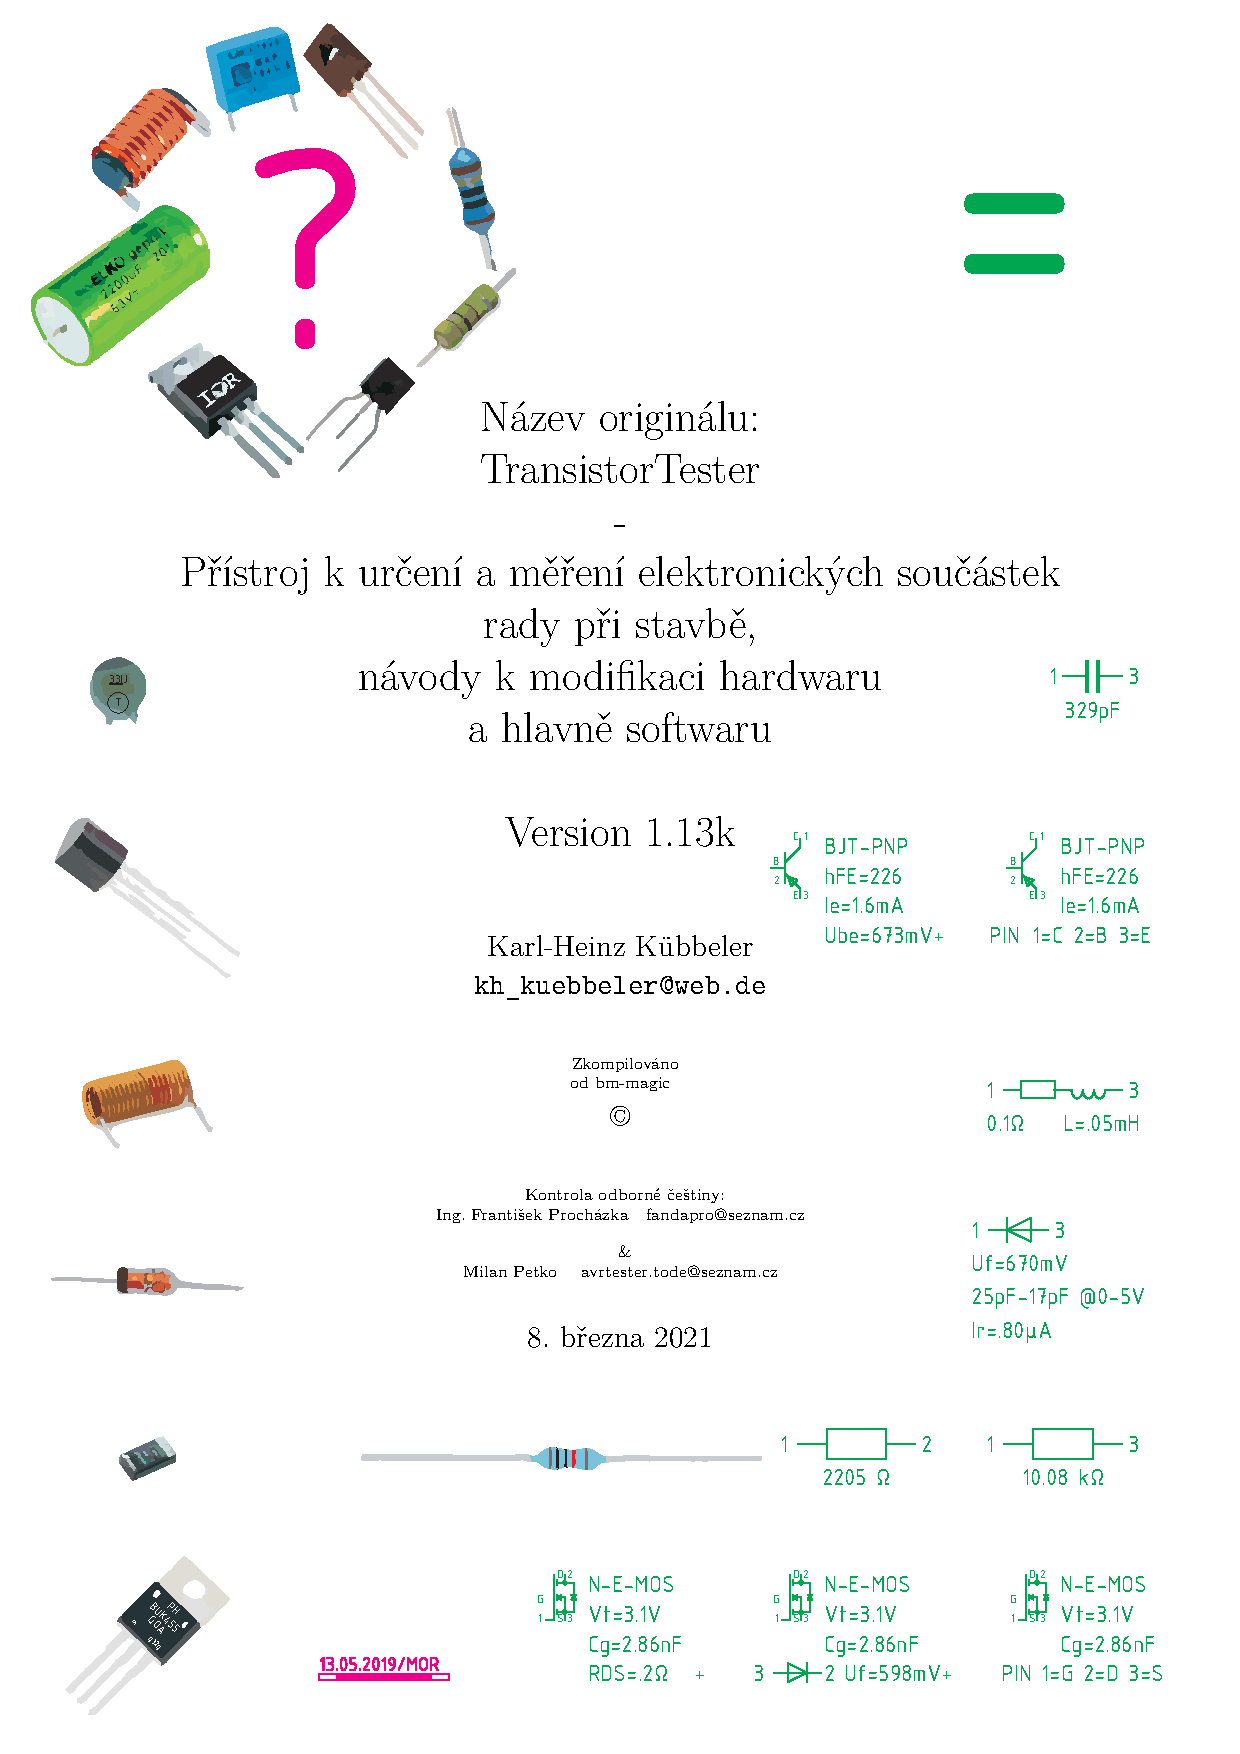
\includegraphics[width=1.0\textwidth]{../FIG/ttester.pdf}
\caption{����� ����� �������}
\label{fig:ttester}
\end{figure}

�������~\ref{tab:display-con} ���������� ���������� ������ D ��� ��������� �������� � �������������� �����������.
��� ���������� SPI ������ LCD-CE ������������ �� ����� ATmega. ���� ������� CE (Chip Enable) ������� ����� 
����� ���� ��������� � GND ������ ����������� ��� � ������ ������� LCD-CE ATmega.

\begin{table}[H]
  \begin{center}
    \begin{tabular}{| c || c | c | c | c | c | c |}
    \hline
           & ����������    & ST7565     & ST7920 LCD     & NT7108 LCD  & SSD1306     & �������������� \\
     ����  & LCD           &   LCD      & serial         & serial      & I\textsuperscript{2}C  & ������� \\
    \hline
    \hline
    PD0    &  LCD-D4       &  LCD-REST  & LCD-REST       & 595-PCLK        &            & \\
    \hline
    PD1    &  LCD-D5       &  LCD-RS    &                & LCD-CS2     &             & ������� 2 \\
    \hline
    PD2    &  LCD-D6       &  LCD-SCLK  & LCD-B0         & 164-595-CLK &  LCD-SDA    & \\
    \hline
    PD3    &  LCD-D7       &  LCD-SI    &                & LCD-CS1     &             & ������� 1 \\
    \hline
    PD4    &  LCD-RS       &            &                & LCD-RS      &             & ������� ������� \\
           &               &            &                & 164-595-SER &             &                \\
    \hline
    PD5    &  LCD-E        &  (LCD-CE)  & LCD-EN         & LCD-EN      &   LCD--SCL  & \\
    \hline
    PD7    &  ������       & ������     & ������         & ������      & ������      & \\
    \hline
    \end{tabular}
  \end{center}
  \caption{���������� ��������� ����� D ��� ����������� ��������� ��������}
  \label{tab:display-con}
\end{table}

����������� ����������� ����� �������� ���������� ������� ����� D ��� �������� �������� LCD-�������. 
� ������� \ref{tab:grid-change} �������� �������� ����������� ��� ������ Strip Grid � ����������� ������������ 
���������� � ���������������� ATmega328.
����� ������� ������������� ������ ������ ��� �������������� �������.
��� ������������� ������������ �������� � ����� ������ Strip Grid (����� STRIP\_GRID\_BOARD=1)
������� ��������� ������� �� ����� ���� ������������, ������ ��� ���� PD4 (T0) ������������.
�� ��� ���������� ������������ � ��������� ������ � ����������� ��������.
� ����������� ������� �������������� �������, ����� ��� ������������� �������� ��� ����������� ����� 
����������� � ������ ������� � ���������� ��������, ������ ��� ��� ������� ������ ������������ � �������
����������� �������.


\begin{table}[H]
  \begin{center}
    \begin{tabular}{| c || c | c | c | c | c | c |}
    \hline
           & ����. LCD    & ST7565 LCD & ST7565 LCD    & ���������������� \\
      ���� &   =1         &   =1       & STRIP\_GRID   & ������� \\
    \hline
    \hline
    PD0    &  ������      &              &             & \\
    \hline
    PD1    &  LCD-D7      &  LCD-SI      & LCD-A0 (RS) & ������� 2  \\
    \hline
    PD2    &  LCD-D6      &  LCD-SCLK    & LCD-REST    & \\
    \hline
    PD3    &  LCD-D5      &  LCD-A0 (RS) & LCD-SCLK    & ������� 1 \\
    \hline
    PD4    &  LCD-D4      &  LCD-REST    & LCD-SI      & ������� ������� \\
    \hline
    PD5    &  LCD-E       &  (LCD-CE)    &             & \\
    \hline
    PD7    &  LCD-RS      &  ������      & ������      & \\
    \hline
    \end{tabular}
  \end{center}
  \caption{���������� ������ � ������ STRIP\_GRID\_BOARD}
  \label{tab:grid-change}
\end{table}

\section{��������� � ���������� � �������}

\subsection{������ ������ ATmega}

��� ������ ATmega �������� ���� �� ���� ��������� ����� ������ �� �������������� �� �������~ \ref{fig:relay_addon}.
� ������ �������� �������� ������������� ���� �������� ATmega ��� ���������� ���������� �������. �������� ����� ���������� ����������, 
��� ������ �������� ���������.\\

�� ������ �������� ������ ��� ������ ������ ��������� ����������� ����������� ������ ATmega ��� ����������� 
������������ � ���������� �����������.\\

������� ��������, ��� �� ���� ����� �� ���� ������ �������� ������ ATmega �� ����������� ������ ������������.
�������, ����� �������������, ����������� ����������� ���������!

\begin{figure}[H]
 \begin{subfigure}[b]{.5\textwidth}
  \centering
  \begin{overpic}[width=.78\textwidth]{../FIG/relay_addon.pdf}
  \color{black}
  \put(78,36){\makebox(0,0)[lb]{\footnotesize VCC or Ubat}}  
  \put(78,32){\makebox(0,0)[lb]{\footnotesize depends on  U{\scriptsize ����}}}  
  \end{overpic}
  \caption{� �������������� ����}
 \end{subfigure}
  ~
 \begin{subfigure}[b]{.5\textwidth}
  \centering
  \includegraphics[width=.78\textwidth]{../FIG/diode_addon.pdf}
  \caption{� �������������� ������}
 \end{subfigure}
 \caption{������ ������ ATmega}
 \label{fig:relay_addon}
\end{figure}

�� ������ �������� ������, ��������� ���� � ����� �������� ���������, ��� �������� �� �������~\ref{fig:relay_um_addon}.
��������� ��� ��������� �����������, ����� ATmega ��������� � ����������  ������. 
������� �������, ��� ������ �� ������� � ������ ���������������� (�����������) ���������.

\begin{figure}[H]
\centering
 \begin{overpic}[width=.58\textwidth]{../FIG/relay_um_addon.pdf}
  \color{black}
  \put(78,42){\makebox(0,0)[lb]{\footnotesize VCC or Ubat}}  
  \put(78,32){\makebox(0,0)[lb]{\footnotesize depends on  U{\scriptsize ����}}}  
 \end{overpic}
\caption{���������� ������ � ����}
\label{fig:relay_um_addon}
\end{figure}

\subsection{��������� ������������� � ����������� ����� 4 V}

���� UART �� ���������, ���� PC3 ����� �������������� � �������� ����������� ����� ��� ��������� �������� ����������. 
���������� ����� ��������� �� \(50~V\) � �������������� ����������� ��������� 10:1. �� ������� ~\ref{fig:zener} 
������������ ����� ��� ��������� ���������� ������ ������������ ��� ������ ������ �� ����� PD7 ATmega. 
������ ���������� ������� ����������, ���� �� ������� ������ \textbf{ TEST} �������. ���, ������������ �� ������� �������, 
��� ���� ����������, ��������, �� \(40~mA\).

\begin{figure}[H]
\centering
  \begin{overpic}[width=.90\textwidth]{../FIG/zener_exp.pdf}
  \color{black}
  \put(5,20){\makebox(0,0)[rb]{\textcolor{red}{external}}}  
  \put(5,17){\makebox(0,0)[rb]{\textcolor{red}{Voltage}}}  
  \put(33,24){\makebox(0,0)[rb]{Can be placed on Tester board!}}
  \put(42,2){\makebox(0,0)[lb]{Should be placed separate!}}
 \end{overpic}
\caption{����� ��� ��������� ���������� �������������}
\label{fig:zener}
\end{figure}

����������� �������� 10:1 ����� ���� ����������� ��� ��������� ������� ���������� ��� ������ ��
���� �������������� ������� � ATmega328. ����������� DC-DC ��������������� ��� ��������� �������������
�� ������, ��� ��� ������ �� ������������ � ������� ��������� �, ��������������, DC-DC ���������������
���������. ����� �������, ����� �������� ���������� ����������� ���� �� \(50~V\) ������ ������������� 
����������, ����������� �������� ����������.\\

\subsection{��������� �������}

�� ���� �������������� �������, ��� ������������� ATmega, ����� ������� ��������� �������.
� ��������� ����� �������������� ����� ������ � ��������� �� \(1~Hz\) �� \(2~MHz\). 
�������� ������ \(5~V\) ����� �������� \(680~\Omega\) ��������� �� �������� ������� TP2.
� �������� ������� GND, ��� ����, ����� ������������ GND DC-DC ��������������� ��� �������� 
������� TP1. �������� ������� TP3 ����������� � GND ����� �������� \(680~\Omega\).
�������, �� ����� ������ ������������ ���� PB2 ��� ����������� ��������� ����� ���������-�������������.
�� ���� ���� ����� �� ������ ��������� ������� �������� ��� ����� ATmega.\\

\subsection{��������� �������}
\label{sec:frequency_counter}

��� ������������� �������������� ������� ��������� �������, ����������� �������������� 
��������� �������. ��� ��������� ������� ������������ ���� PD4 (T0/PCINT20) ATmega. 
���� �� ���� ������������ ��� ����������� LCD-�������. � ����������� �������� � ����� PD4 ��������� 
������ LCD-RS, � �������� strip grid - ������ LCD-D4. ��� ����� �������� ���� PD4 ����� ���� ���������� 
�� ����, ���� � ������ ������ �� ��������� �������� ���������� �� LCD-�������.\\
 
������, ����� ������������ �������������� ����� �����������, ������������ �� �������~\ref{fig:FreqMes}.
���������� �� ������ ����� PD4 (LCD-RS ��� LCD-D4) ������ ���� ����������� ����� \(2,4~V\) ��� ����������� 
ATmega ��� ���������� �� ����� ��������� ������� ATmega, ����� �������� ������ ���������������� � �������� 
�������. �� ����� ����������� LCD-������� ������ ���� ����������, ������ ��� ������������� ��������� 
���������� ����� �������� ������������� ����������.

\begin{figure}[H]
\centering
\includegraphics[width=.4\textwidth]{../FIG/Frequency_addon.pdf}
\caption{�������������� ����� ��� ��������� �������}
\label{fig:FreqMes}
\end{figure}

\subsection{������������� ����������� ��������}

��� ����� �������� ������� � ���� �������������� ������� ��� ATmega328, �� ������ ��������� �����, ���������
��������������� ������� � �������.   
�������~\ref{fig:RotExt} ���������� ����� ����������� � ������� � ���������� LCD.
��� ������� ��� ����������� ����������� ���������������� �������� �������� � ������� 
����������� LCD. �� �����, ������������ �������� ��� ����������� ������������ ��������.
�� ������ ������� ����������� LCD ������ �� ���������� ����� � ��������� � ���������, ���������������
��� ����������� ����������� LCD. ����� �������, ������������ � ���� ������� ����� ��������.    

\begin{figure}[H]
\centering
 \begin{overpic}[width=.30\textwidth]{../FIG/rotary_extension.pdf}
  \color{black}
%  \put(47,6){\makebox(0,0)[lb]{Taster}}    
 \end{overpic}
\caption{����� ����������� ����������� ��������}
\label{fig:RotExt}
\end{figure}

�� �������~\ref{fig:RotEnc} �������� ����������� ������ ���� ����� ���������� ��������������� 
���������.
� ������ 1 ������ ������������������ ��������� �������������� ���������� ��� �������� �� ��� 
������������� ���������. ���������� ������ ������ � ��� ���� ������ ��� ���������� �������������
��������� �� ������ ��������.
� ������ 2 ��� �������� �� ���� ������������� ��������� ������������ ������ ���� ��������� ���������. 
� ���� ������ ���������� ������������� ��������� ������������� ���������� ������ �� ������ ��������.  
������, � ����� ���������, � ������ ������������� ��������� ��������� �������������� ������ 
���������.
\begin{figure}[H]
\centering
 \begin{overpic}[width=.87\textwidth]{../FIG/rotary_encoder.pdf}
  \color{black}
  \put(90,71.5){\makebox(0,0)[lb]{������� A}}
  \put(90,62){\makebox(0,0)[lb]{������� B}} 
  \put(90,29){\makebox(0,0)[lb]{������� A}}
  \put(90,19){\makebox(0,0)[lb]{������� B}}
  \put(6,6){\makebox(0,0)[rb]{\footnotesize ���������}}    
  \put(6,48.5){\makebox(0,0)[rb]{\footnotesize ���������}}    
  \multiput(23.5,53)(24.6,0){3}{\footnotesize ������}
  \multiput(11,10)(12.3,0){6}{\footnotesize ������}
  \put(52,43){\makebox(0,0)[cb]{{\large ������ 2}}}
  \put(52,1){\makebox(0,0)[cb]{{\large ������ 1}}}      
 \end{overpic}
 \caption{����������� ���� ����� ���������� ��������������� ���������}
 \label{fig:RotEnc}
\end{figure}
�������~\ref{fig:RotBounce} ���������� ������ ��������, ������� ����� �� ������ �������� ���������
�� � ������������ ��������� ������������� � ����� ��������. ������ ��������� 
��������� �������������� ������������ ���������� � ����������� � ����������� �����.
�������, ��������� ��� ��������� �������������� ����� ��������� ����� ������� ��������� ���������.
��� ������� ����� ������������ ���������, � ����� ��������� ������ ������������������ ����� ���� 
���������� ��� ������� ����������� ��������.

���� �� ���� ������������� ������� �������������� ����, ������, ���� ��������� ��������������, �� ��� �����������
�������� ���������� �������������� ��������� ������������� � ����� ������ (WITH\_ROTARY\_SWITCH=2 ��� 3).

���� ��� ��������� ������� ����� ��������� �������������� ��������� ������� �� ��� �������������
�������, ��� �������� �� �������~\ref{fig:RotBounce}, �� ������ �������������� ������������������
������������ � ���� ������� (WITH\_ROTARY\_SWITCH=1).

��� ��������� ��� ��������, �� ������ ������� ����� ���������������� � ���� ��������. �������� 
2 � 3 ������������� ������ ����������������, 1 ������� ���������������� � 5 ������� ����������������.

������� ��������� (���������� �������, ���������� �����) ����� ���� ��������� �������� 
������������� ���������, ��, � �� �� �����, ����� ���� ������� ��-�� ������������� ��������� 
��������� �������������� � ����� ��������.
\begin{figure}[H]
\centering
 \begin{overpic}[width=.87\textwidth]{../FIG/rotary_bouncing.pdf}
  \color{black}
  \put(90,39){\makebox(0,0)[lb]{�������� A}}
  \put(90,30){\makebox(0,0)[lb]{�������� B}}
  \multiput(12,23)(28,0){3}{\footnotesize �������}
  \put(7,20){\makebox(0,0)[rb]{���������}}
  \put(5,12){\makebox(0,0)[lb]{��������� ��������� ����� �������:}}      
 \end{overpic}
 \caption{������� � ���������� ��������� ��������������}
 \label{fig:RotBounce}
\end{figure}	
���� ������� �� �������� ��� �� ������������� ��-�� �������������� �����������, ������ ���� ��������� ��������, 
�� ������ ������������ ��� ����������� ������ ��� ����������� ������� � �����.
� ���� ������ �������� ����� WITH\_ROTARY\_SWITCH, ��� ���������� ������ ���������, ������ ���� ����������� 4.

\subsection{����������� ������������ �������}

������� ������� Wolfgang Sch. �� ����������� ������ �� ��������� �������� ��������� ������ ������� � ������������ ST7565.
� ��������� ����� �� ����� ������ ���������� ����������� LCD (128x64 ��������) � ������������ ST7565. 
��������� ���������� ST7565 ������������ �� ����������������� ����������, �� ������ ������ ����������
����� ������������. ��� ������ ����� D ATmega ����� ���� ������������ ��� ������ �����.
ATmega ��������� ������ �����, �� ������� ����, \(32~kB\) ����-������ ��� ��������� ������������ �������.
ST7565 ���������� ���������� ������� ���������� \(3,3~V\).
������� ��������� �������������� ������������ \(3,3~V\).
������������ � ����������� ST7565 �� ��������� ������� ����������� ���������� 
�������� ������ \(5~V\). ��� ������������ ���������� ������� �������� \(5~V\) � \(3,3~V\) ����� ������������
�����, ����������� �� ������� \ref{fig:ST7565lcd} � �������������� 
���������� ��������������� ������� 74HC4050.
�� ������ ����������� ��������� ������ ������� ��������� 74HC4050 ������ ���������, �������� \(2,7~k\Omega\).
������� ���������� �� ���������� ������������ ���������� ���������� �� ������ ������������ ����������� ������ ���
���������� ������� \(3,3~V\), � �������������� ����� �� ������ ������������ ����������� �� �������� ��������� 
��������� ������� \(5~V\) �� ATmega.
�� ������ ���������, ��� ����� �������� � ���������� ����� ���� ��������� ���������� ������� ����������� ST7565.
 
� ����� ������, ��� ���������� ��������� ���������� 74HC4050 ����� ������� �� ����� ������������ ����������� 
������ ������������� ����� ��������� ������� � ATmega. 

\begin{figure}[H]
\centering
 \begin{overpic}[width=.814\textwidth]{../FIG/ST7565lcd.pdf}
  \color{black}
  \put(88,10){\makebox(0,0)[lb]{Background}}
  \put(88,7){\makebox(0,0)[lb]{LED}}
 \end{overpic}
\caption{����������� ������������ ������� � ������������ ST7565}
\label{fig:ST7565lcd}
\end{figure}

� ������� \ref{tab:spi-processor} �������� ������ ������������ ����������� ATmega328 
��� ������ ����������������� �� ���������� SPI (LCD\_INTERFACE\_MODE=4) ��� ��� ��������������
���������� (LCD\_INTERFACE\_MODE=3).
��������� ���� ������������� ��� ������ ���� ���������� ����� ���� ������� � ������� �����
� makefile STRIP\_GRID\_BOARD.
���������� ��������� ������� ���������� � ����� config.h.
���� ��� ����� ���� �����������, �� ������ ��������� ����� ����� ���� ��� 
����� STRIP\_GRID\_BOARD � ������ ��������� ����������� � ����� config.h.

\begin{table}[H]
  \begin{center}
    \begin{tabular}{| c || c | c | c | c | c | c | c |}
    \hline
 ����������  & m644  & m1280 & m1280  & m328 & m328 & m328 & m328 \\
STRIP\_GRID\_BOARD &       &   -   &   1    &  -   &  1   &  2   &  5   \\
������:     &       &       &        &      &      &      &     \\
    \hline
    \hline
  RES       &  PB4  & PA0   &  PA4   & PD0  & PD4  & PD0  & PD2 \\
    \hline
  EN, CLK   &  PB6  & PA2   &  PA2   & PD2  & PD2  & PD2  & PD3 \\
    \hline
  RS, D/C   &  PB5  & PA1   &  PA3   & PD1  & PD3  & PD3  & PD1 \\
    \hline
  B0, MOSI  &  PB7  & PA3   &  PA1   & PD3  & PD1  & PD1  & PD4 \\
    \hline
  CE, CS    &  PB3  & PA4   &  PA5   & PD5  & PD5  & PD5  & PD5 \\
    \hline
    \end{tabular}
  \end{center}
  \caption{����������� �� SPI ��� ��������� ������������}
  \label{tab:spi-processor}
\end{table}

������ ST7565 ��� SSD1306 ���������� ������������ �� 4-���������� SPI ����������.
�� � ������������ SSD1306 �� ����� ������ ���������� ��������� �� ���������� I\textsuperscript{2}C ����������� PD2 
��� SDA � PD5 ��� SCL ������.
������� SDA � SCL ������ ���� ��������� ����������� ����� \(4,7~k\Omega\) � ���������� \(3,3~V\).
������ ����������� OLED ������� ������� �� �������~\ref{fig:ssd1306i2c}.
������� ���� I\textsuperscript{2}C ����������� ������ ����� ������������ ������ ATmega � \(0~V\).
����� ������������ ������������� ���������� � ���������� \(5~V\), �� ������ ���������, ��� ��� ����������
��������� ������� ������� \(5~V\). ������ ����� ����������� ������� �������� �������, ������� �������� ������� 
������� �� \(3,3~V\). 
�� ������ ���������, ��� � ATmega �������� ��������� � ���������� ���������� I\textsuperscript{2}C �� ����,
��� ������� ����� �����������. ���� �� �������� � ���������� �������������� � ���������� ������� ����������,
�� �� ������� ATmega ����� �������������� ������� � ������� \(5~V\).

���, ��� � ��������� ������� �� ���������� ����� ������ OLED ����� ���� \(VCC\), ����������
���������� �������������� �������� �� ����������������� ��������� \(68~\Omega\) � ��������������� ������������ \(10~\mu F\). 
������ \(68~\Omega\) ��������� ����� ����� ������������ ������������� \(1~mH\).
��� ��������������� ������� ��� ������ � �������� OLED ��������� ���������� ���� � ����������� ���������� ������������.

����� ����� ��������� ������������ ������� ������ OLED �������. ��������� ������ ����� ������� � ������������ \(GND\) � \(VCC\).   
 
\begin{figure}[H]
\centering
\includegraphics[width=.814\textwidth]{../FIG/SSD1306_I2C.pdf}
\caption{����������� ������������ OLED ������� � I\textsuperscript{2}C �����������}
\label{fig:ssd1306i2c}
\end{figure}

��� ����������� � ������������ ����� ATmega644 ������ ������ PB3 (SCL) � PB4 (SDA) ������������ ����� PD5 � PD2.
��� ����������������� ����� ATmega1280 ������������ �������� PA5 (SCL) � PA4 (SDA).
��� ������ ����������� ������� �� ����������� ����� ������������ ���������� �������� �����-������� � ��������
����������� ����������� LCD, ��� ��� ��� ������� � ������� �� ��� ��������.

������� ����� ���������� ������� � ������������ ST7920, ������ ��� ���������� ������������ ���������� ������� \(5~V\).
������� ������ ������������ ����� 128x64 �����.
������ ������� � ������������ ST7920 ����� ���� ��������� �� 4-bit ������������� ���������� ��� �� ������������,
����������������� ����������, �������� ������� \ref{fig:ST7920lcd}.

\begin{figure}[H]
\centering
 \begin{overpic}[width=.698\textwidth]{../FIG/ST7920interface.pdf}
  \color{black}
  \put(20,1){\makebox(0,0)[cb]{serial mode}}  
  \put(80,1){\makebox(0,0)[cb]{4-bit parallel mode}}   
 \end{overpic}
\caption{����������� ���������� � ������������ ST7920}
\label{fig:ST7920lcd}
\end{figure}

��� ���� ����� ����������� ���������� � ������������ ST7920 � Makefile ������ ���� ����������� ����� 
�WITH\_LCD\_ST7565 = 7920�. ����� ����, ��� ����������� �� ����������������� ����������, 
���� ���������� � ����� �CFLAGS += -DLCD\_INTERFACE\_MODE=5�.

� �������~\ref{tab:ser-processor} �������� ����������� ��������� ����������������� ��
����������������� ���������� � ������� INTERFACE\_MODE 5 (ST7920) � 7 (SSD1803).

\begin{table}[H]
  \begin{center}
    \begin{tabular}{| c || c | c | c | c |}
    \hline
 ����������  & m644  & m644 & m1280  & m328 \\
STRIP\_GRID\_BOARD &   -   &   1   &        &     \\
������:     &       &       &        &         \\
    \hline
    \hline
  EN        &  PB3  & PB6   &  PA5   & PD5     \\
    \hline
  B0, R/W   &  PB4  & PB7   &  PA4   & PD2      \\
    \hline
  RESET     &  PB2  & PB4   &  PA0   & PD0      \\
    \hline
    \end{tabular}
  \end{center}
  \caption{����� ��� ����������������� ����������� ��������� ������������}
  \label{tab:ser-processor}
\end{table}

��� �� ��� � � ������ ���������� ������ ����������� �����������, ��� ������� � ������������ ST7920,
������� LCD\_ST7565\_H\_FLIP � LCD\_ST7565\_V\_FLIP ����� �������� ���������� ���������� �����������.

������ ������� �������� ����������� �������� � ������������ NT7108 (KS0108, S6B0108). ��������� ��� ������� 
���������� ������ ������������ 8-������ ���������, ���������� ���������� ��������������� - ������������� 
��������������� �����������. ���������� ������ -- ������������� ���������� 74HCT164 ��� 74HCT595.
������� ������ ����������� ������� �� ������� \ref{fig:NT7108lcd}.

\begin{figure}[H]
  \begin{subfigure}[b]{.5\textwidth}
    \centering
    \includegraphics[width=.9\textwidth]{../FIG/ST7108serial164.pdf}
    \caption{� �������������� 74HCT164}
  \end{subfigure}
  ~
  \begin{subfigure}[b]{.5\textwidth}
    \centering
    \includegraphics[width=.9\textwidth]{../FIG/ST7108serial595.pdf}
    \caption{� �������������� 74HCT595}
  \end{subfigure}
  \caption{����������� ������������ ������� � NT7108 ������������}
  \label{fig:NT7108lcd}
\end{figure}

��� ��� ��������� ������ LCD ����������� �� ������������ �������, ����� ������������ �� ������ ��������� �������� 
������ �������. 
��������� �������� � ������������ ������� ��� ����� LCD ABG128064 ��������� � �������~\ref{tab:NT7108types}.

\begin{table}[H]
  \begin{center}
    \begin{tabular}{| c || c | c | c | c |}
    \hline
           & 128064H  &  128064G  & 128064C  & 128064B \\
    ������ &         &          &         &         \\
    \hline
    \hline
  VDD (5V) &   1     &  2       &   4     & 2       \\
    \hline
  VSS (GND) &   2     &  1       &   3     & 1       \\
    \hline
 VO (Drive) &   3     &  3       &  (5)    & 3       \\
    \hline
  DB0-DB3   &   4-7   &  7-10    &   9-12  & 7-10    \\
    \hline
  DB4-DB7   &   8-11  &  11-14   &   13-16 & 11-14   \\
    \hline
  CS1       &   12    &  15      &   1     & 15      \\
  CS2       &   13    &  16      &   2     & 16      \\
    \hline
  Reset     &   14    &  17      &   -     & 17      \\
    \hline
  R/W       &   15    &  5       &   7     & 5       \\
    \hline
  RS        &   16    &  4       &   6     & 4       \\
    \hline
  E         &   17    &  6       &   8     & 6       \\
    \hline
  VEE       &   18    &  18      &   -     & 18      \\
    \hline
  LEDA      &   19    &  19      &   17    & (19)      \\
  LEDK      &   20    &  20      &   18    & -      \\
    \hline
    \end{tabular}
  \end{center}
  \caption{�������� � �������� NT7108 �������}
  \label{tab:NT7108types}
\end{table}

� ������� \ref{tab:7108-processor} �������� ����������� �� ����������������� ���������� ����������� 
NT7108 � ��������� �����������������.
\begin{table}[H]
  \begin{center}
    \begin{tabular}{| c || c | c | c |}
    \hline
����������  & m644  &  m1280  & m328 \\
������:     &       &        &         \\
    \hline
    \hline
  EN        &  PB3  &  PA5   & PD5     \\
    \hline
  RS        &  PB2  &  PA4   & PD4      \\
  B0        &  PB2  &  PA4   & PD4      \\
    \hline
  CS1       &  PB7  &  PA3   & PD3      \\
    \hline
  CS2       &  PB5  &  PA1   & PD1      \\
    \hline
  CLK       &  PB6  &  PA2   & PD2      \\
    \hline
  PCLK      &  PB4  &  PA0   & PD0      \\
    \hline
    \end{tabular}
  \end{center}
  \caption{����������� ����������� � NT7108 �� ����������������� ����������}
  \label{tab:7108-processor}
\end{table}

�� ����� ������ ������������ ������� � ������������ PCF8814, ������� ������ ������������, 
��������, � Nokia 1100. 
�� ������ ���������, ����� ��������� ����������� ������������ � ����� ������ �������.
���������� PCF8814 ����� ������������ SPI-��������� 3-� ��������� ��� 4-� ���������, 
I\textsuperscript{2}C-��������� � ����������� 3-� ���������, ������� ��� ������ 
������/������� � �������� ������� ���� � 8 ������ ������.
������, ��� ������� ������������ ������ 96�65 ��������, ������� ������ ��� ������������ �� ������������ 
� ���� ������������. ����� ����������� ����� �� ����� ��� ���������� �������. 
��� � ����������� ����������� ��������, ���� ���������� �������� � \(3,3~V\). 
������� ��������� ��������������� ������� ���������� �������� ��� \(5~V\) ������� ATmega.
��� SPI ���������� � 3-� ���������� ���������� �� ������ ������������ ����� � makefile
LCD\_SPI\_OPEN\_COL (��������� ��������� ������ ATmega).
�� ������ ������������ �Pull-Up� ��������� ��� �� ������������� 
����� PULLUP\_DISABLE � makefile.  
� ��������� ����� � ������������ PCF8814 ������������� ������ 3-� ��������� ���������.

\begin{table}[H]
  \begin{center}
    \begin{tabular}{| c || c | c | c | c |}
    \hline
     ����  &  PCF8814    & PCF8814        & PCF8814     & �������������� \\
           &    SPI      & 3-� ���������  & I\textsuperscript{2}C  & ������� \\
    \hline
    \hline
    PD0    &   LCD-RESet  & LCD-RESset       &            & \\
    \hline
    PD1    &   LCD-D/C   & LCD-SCE        &             & ������� 2 \\
    \hline
    PD2    &   LCD-SCLK  & LCD-SCLK       &  LCD-SDIN   & \\
    \hline
    PD3    &   LCD-SDIN  & LCD-SDIN       &             & ������� 1 \\
    \hline
    PD4    &             &                &             & ������� ������� \\
    \hline
    PD5    &             & LCD-EN         &   LCD-SCLK  & \\
    \hline
    \end{tabular}
  \end{center}
  \caption{���������� ��������� ��� ��������� ����� ����������� ����������� PCF8814}
  \label{tab:PCF8814-con}
\end{table}

�������� ��� ��� ��������� ����������� PCF8812 � 102x65 �������� ����� ����������, 
��, ����, �� ������������.

\subsection{����������� ������������ �������� �������}

� ������������ ��������� ��������� ����������� ������� ������ ������� �������� � ����������� SPI.
�� ������� \ref{fig:Color_both} ������� ��� ����� ���� �������������� �������� � 128x128 � 
128x160 ��������.
������ ������� ����� ���, ������� ����� � ������� ����� ������.
��, � �����, ������� ��� ������ � �����.

\begin{figure}[H]
\centering
\includegraphics[width=.46\textwidth]{../PNG/Color_ILI9163_ST7735.jpg}
\caption{��� ����� ���� ������� LCD}
\label{fig:Color_both}
\end{figure}

������ 128x128 �������� ���������� ���������� ILI9163.
������ 128x160 �������� ���������� ���������� ����� ������� � ST7735 �����������.
������ ������������� � ������ ��������, ������� ��������� ������� SPI � ������� ������� ��� 
����������� ����������� ��������. ��������� �������� ������� \(5~V\) �������� ATmega � ������ \(3,3~V\) 
�������� ������ ����������� �������������� ����������������� \(10 k\Omega\) �����������.
������� ��������� (LED) �����������, �.�. ��� ��� ��������� ���������� ���������� ��������.
��-�� �������� ���������� �� ��������� ����� ���������� ��������� ��������� ����� � ���� �������.
��� ������� 128x128 �������� ����� ���������� 8 ����� ������ ������� 12x8,
��� ������� 128x160 �������� ������� 10 ����� ������.
�� ������� \ref{fig:Color_PNP} �� ������ ������ ��������� ��������� ������������ �����������
�� ������� 128x128 ��������.

\begin{figure}[H]
\centering
\includegraphics[width=.46\textwidth]{../PNG/Color_PNP_ILI9163.jpg}
\caption{��������� ����������� PNP �����������}
\label{fig:Color_PNP}
\end{figure}

��������� ������� � ��������� ����� �� ������������.
���� ���� � ���� ������������ ��������� ����� �������� � ����� lcd\_defines.h ���
� Makefile.
���������� ���������� ����������� 16-������ ���������� ����������. ���� ������������ ���������� ����� 
���� ������� ���������� LCD\_FG\_COLOR, � ���� ��������� ���������� LCD\_BG\_COLOR .



\section{�������� �� ������ ������� }

� ������� ����� �������������� LCD-������� 2x16, ���������� ����������� � HD44780 ��� ST7036. �� ������ ��������� ���, 
����������� ��� ���������, ��������� LCD-�������� ����� ��� ����, ��� ������. � ������� ��������� OLED-�������, �� �� 
���� �������� ����� ��� ���������� ��� ATmega, � � ��� \textbf{ ��} ����������. ����� ������������� OLED-������� ������� 
�������� �������� ������������ ������� ��� ����������� ���������.\\

����� �������� ������������ �������� ���������, ��������� R1 - R6 \(680~\Omega\) �
\(470~k\Omega\) ������ ���� ������� (0,1\%). � ������� ����� �������������� ATmega8, ATmega168 � ATmega328. ��� 
����������� ������������ ��� �������, ������������� ���������� ATmega328.\\
 
������� �� ������ ������� ��� �������� ������� �� �������� ����� ��� ����������������. � �������� IC2 ������������� 
������������ ������������ � ����� �������� ���������� MCP1702-5002, ������ ��� �� ���������� �����  \(2~\mu A\) � ����� 
�������� \(5~V\) ��� ������� ���������� ����� \(5,4~V\). �� �� ����������� �� ������� � ��������� 78L05 � ������� TO92 .\\

����� �������� ������������ �������, ���������� ������������ ������� ��� �������� ������� � ����� ��� LCD-������� � 
����������������. ��� ������� ������ \textbf{ TEST} ������ �������������� ���������� \(5~V\) �� ������� ������� 
���������������� � LCD �������. ���� ��������� ������ \textbf{ TEST}, ���������� ������ ���������. ����  ���������� 
� �����, �� ���������� ��������� �������, \textbf{ ���������} �������� ��������������� � ���������� LCD-�������. 
����� ������������ LCD ������� ���������� 
����������� ��������� ������������ ���������� ������� ������� LCD ������� (�.�. �� ��������� LCD �������� ��� 
���������� ��������) � GND � VCC ����� �������!\\
 
���� �� �������, ��� ��� � �������, ����� ������������ �������. ���� �� ��� ����������������� ATmega, �� ������ 
�������������� ������ ������ \textbf{ TEST}. ��� ��������������� ������� ������ \textbf{ TEST} ��������� LED1 � ��������� 
LCD-������� ������ ����������. 
���� �� ���������� ������ \textbf{ TEST}, ��������� LED1 �� ������ ������� ��� ������� ��������� ������ 
(������� �� ������������� ���������� ��� ����������� ������������ �����������). 
��������, ��� ����������� ����������� ��� ���������������� ������ ���� ��� ������������� ���� ����������������. ��������� ��� ATmega8 �� �������� �� ATmega168!


\section{��������� ��� ������ ������� Markus F.}
\label{sec:change_markus}
\begin{description}

\item[�������� ����������.]
�������� ����������� ��������� �������: ������ ���������� ����������� ��� ������ ���������. �������� ����� ����� 
��������� ������ (Makefile) �������� �� ���������� ���������� ������� ATmega �� \(4,3~V\). ���������� ��� ��������� 
�������: ���� PD6 �������� �������� ����������� C2 \(100~nF\) �� ������ VCC, ��� �������� ������ ���������� 
VCC (\(5~V\)). ��� ������� �������� ����������� C2 ����� ���� �������� �� \textless~\(10~nF\). ���� ��������, 
�� �������� ��������������� � ���� PD6  �������� �������������� ����� \textgreater~\(220~\Omega\).
\item[��������� ������� �����.]
	���� ������ ����������� ��� ������� �� ������ \textbf{ TEST}, �� ���� ����� �� �����������, �� ����� ������� ���� �������� 
� �������. �������� ��������� ������� ����� ��������� LCD-�������. �������� R7 � ���� P-N-P-����������� T3 ��� 
��������� \(27~k\Omega\), 
����� ��������� ����������� �������. ����� �������� ������������ ���  ����� ������ ���������� ������� ��� ��� ������ 
������������ �������� P-N-P ����������� T3, ���������� ��������� ������������� �� \(3,3~k\Omega\).
\item[�������������� ������������� �������� ����� PD7.]
���������� �������������� ���������, ����� ��������� �������, ������ �������������  ����������� ������� � ���������� 
�Timeout�. ����������� ����������� ����������� � ������ PULLUP\_DISABLE, �. �. ��� ���������� ������������� ��������� 
		���������. �� ���� ������� ���������� ����� PD7 �� ����������, ���� ������� �� ���������� ������� \textbf{ TEST} ��� 
������������ T2 � GND. ������� �������� �������������� \(27~k\Omega\) � VCC ������ ��� ��������.
\item[����������� C1 � AREF.]
������ ���������� �� �������� AREF ����������� �� \(100~nF\) ��� ��, ��� � Markus F. ���� �� ���� ������������� ������ 
������� ���������� ��� - ��� ���� ������� ��������. ����������� ����������� ��� ATmega168 � ATmega328 ���������� 
�������������� ����� ����������� �������� ���������� ��� \(1,1~V\), ���� ������� ���������� ���� \(1~V\). ��� ��������� 
�������� ���������� ��� ��� ��������� ������� �����������. � ���������, ������������ �������� ���������� �� \(5~V\) �� 
\(1,1~V\) ���������� ����� ��������. �� ���� ������� ����� ��������� �������������� ����� �������� \(10~ms\). 
��� ���������� �������� ������������ �� \(1~nF\), ��� ����� ����� ���� ����������� ���������. � �� ������� ��������� 
�������� ��������� ��� ���� ���������. ���� � �������� ������������� ��� ������������� ��������� ����������� 
���������. ���� �� ������������� �������� ����������� �� \(100~nF\), �� ������ ��������� ����� NO\_AREF\_CAP
� Makefile, ��� ��������� ���������� ������� �������� � ���������.
\item[��������� ������ �� \(8~MHz\).]
�� ������ ���������� ����� �� \(8~MHz\) � ������ ������� �������� ����� ��������������� � ������ PB6 � PB7 
(������ 9 � 10). ��� ����������� ��������� ���� ������� ��� ������������� \(22~pF\) � �������� ������ �� ����� 
������������ ATmega. �� ��� �� ������, ������ �����, ������������ ���������� ��������� �� \(8~MHz\) ��� ��������� 
������� ���������� �� ������� ��� ���������� ���������� �������� ��������.
\item[����������� ��������� ����������.]
� ������������ ����� Markus F. �������� ������ ���� ����������� \(100~nF\) �� ���������� VCC. ��� �� ���� ���������� 
����������. �� ������, �� ������� ����, ������������ ������������ �������� \(100~nF\) ����� ������� ������� ATmega � 
����� ������� ����� � ������ ������������� ����������. �������������� ������������ \(10~\mu F\)
(����������������� ��� ����������) �� ����� � ������ ������������� ���������� �������� ������������ ����������. 
���������� SMD �����������  \(10~\mu F\) ����� ������������ �� ������� �������� �������, � �� ����� ������ ����� 
������ �������� ESR.
\item[����� ���������������� ATmega.]
��� �������� ������� ������� �������� ������������� ATmega8, Flash ������ � ��� ������������ ����������� �� 100\%.
��mega168 ��� ��mega328 ���������� �� ������� � ATmega8, � ���� ������������� ������. 
��� ������������� ATmega168 ��� ��mega328 �� ��������� ��������� ������������: 
\begin{itemize} \setlength{\itemsep}{-1.5em}
 \item ������������ � �������������� �����������.\\
 \item ��������� �������� ��������� � �������������� ������������� �������� ���.\\
 \item ��������� ��������������  ��� ������������� ���� \(2100~\Omega\).\\
 \item ��������� �������� ESR ������������� � �������� ���� \(20~nF\).\\
 \item ��������� ���������� ���� \(10~\Omega\) � ����������� \(0,01~\Omega\).\\
 \item ������������� ����� PC3 � �������� ����������������� ������ ��� ����������� ����� ��� ��������� �������� ����������.\\
\end{itemize}
\item[������������� ������������ ������� ����������.]
����������� ����������� ������ ���������� ����������� �������� �������� ���������� �� ������ PC4. � ���� ������ ��� 
��������� ������� �� ������ ������ LCD-������� ������ ��������� ��������� �No VCC = x.xV�. ���� ��� ��������� 
���������� ��� ������������� ���, �� ������ ���������� �������� \(2,2~k\Omega\) ����� ������� PC4 � VCC.

\end{description}

\section{����������� ����� � ATmega644 ��� ATmega1284}

����������� ����� ��� ������������ ATmega644/1284 ����������� ��������� � Nick L. �� �������.
����� \ref{fig:t644tester} ��������� ��������� �������� ���������� ������, � ����� �������� ����� 
������������ �������. 
���� ����������� ����� ����� ��������� ����� �� ������� \ref{fig:ttester}, 
���������� ������ ��������� ����������.
���������� ������� �� ����� \ref{fig:RotExt} ������ ���� ��������� � PB5 � PB7 (������ PD1 � PD3).
��� �������, � ����� VCC � GND �������� �� ������� ���������������� ISP. ����� �������, �����������
����������� �������� �� ������ ������� �����������.
�������� 16:1 � 74HC4060 ������ ������������ ��� ������ ���� \(2~MHz\). 
�� ����� ����� ���� ����������� ��� ������ �� \(24~kHz\) �� \(400~kHz\) ��� ��������� ��������
��������� ������� � ������� �������� �������.
��� ���������� ������������ (�������� ������� � ��������� ���������) ������������ 
���������� ������������� 74HC4052.
������� \ref{tab:mega644-display} ���������� �������� ����������� ������� � ������ 
ATmega324/644/1284.
����������� ���������� � �������������� ���������� I\textsuperscript{2}C �������� ������ ��� ����������� � 
������������ SSD1306.
������� ���������� I\textsuperscript{2}C ������� ��������� ������������� ���������� \(4,7k\Omega\) � ���������� \(3,3~V\).
������� ���� I\textsuperscript{2}C ����������� ������ ����� ������������ ������ ATmega � \(0~V\).

\begin{figure}[H]
\centering
\includegraphics[width=1.\textwidth]{../FIG/t644tester.pdf}
\caption{����������� ����� ���������� ������� � ATmega644}
\label{fig:t644tester}
\end{figure}

\begin{table}[H]
  \begin{center}
    \begin{tabular}{| c || c | c | c | c |}
    \hline
      ���� & ���������� & ����������� LCD & ����������� LCD & ��������������\\
	   &     LCD    &   SPI 4-wire &   I\textsuperscript{2}C      &  ������� \\
    \hline
    \hline
    PB2    &  LCD-RS         &            &          &       \\
    \hline                                              
    PB3    &  LCD-E          &  (LCD-CE)  &  LCD-SCL &       \\
    \hline                                              
    PB4    &  LCD-D4         &  LCD-REST  &  LCD-SDA &       \\
    \hline                                              
    PB5    &  LCD-D5         &  LCD-RS    &          & ISP-MOSI \\
           &                 &            &          & ���������� ������� 2 \\
    \hline                                              
    PB6    &  LCD-D6         &  LCD-SCLK  &          & ISP-MISO \\
    \hline                                            
    PB7    &  LCD-D7         &  LCD-SI    &          & ISP-SCK  \\
           &                 &            &          & ���������� ������� 1 \\
    \hline
    \end{tabular}
  \end{center}
  \caption{����������� �������� � ������ ATmega324/644/1284}
  \label{tab:mega644-display}
\end{table}

�� ����� ������ ���������� ������� � ������������ NT7108 (KS0108, S6B0108) � �������, ���������� �� ATmega644 ��� ATmega1284
��������� ��������� ����� ����������� ���������� �� �������~\ref{fig:NT7108lcd_644}.
�� ����� ������ ��������� �������� � ���������� ��������� ���������� ������� � ������������� NT7108, 
��� �������� � �������~\ref{tab:NT7108types} �� ��������~\pageref{tab:NT7108types}.

\begin{figure}[H]
  \begin{subfigure}[b]{.5\textwidth}
    \centering
    \includegraphics[width=.88\textwidth]{../FIG/ST7108serial164_644.pdf}
    \caption{��� ������������� 74HCT164}
  \end{subfigure}
  ~
  \begin{subfigure}[b]{.5\textwidth}
    \centering
    \includegraphics[width=.88\textwidth]{../FIG/ST7108serial595_644.pdf}
    \caption{��� ������������� 74HCT595}
  \end{subfigure}
  \caption{����������� ������� � ������������ NT7108 � ATmega644/1284}
  \label{fig:NT7108lcd_644}
\end{figure}

\section{����� � �������������� ATmega1280 ��� Arduino Mega}

������ ����� ���� ������ � �������������� ���������������� ATmega1280 
��� ATmega2560, � ����� �������� �� ���� Arduino Mega.
����� �������� �� �������~\ref{fig:t1280tester}.
���������� ��������� Arduino ��� ����������� ������� ������� ������� ������.
����������, ���������� ������� ������, �� ����������� ��� ���������� ������ �������.
���������� ATmega2560 ����� ������� ���������� ������, �� ������ ���� ����
����� �������, ����������� ��� ����� ������� ��������� �������.
���� ������ ���� ������������ ��������/��������� ��� �������� ������� ��������� �
������������ ������� ���������� ��� ��������� ������ �������.
����� ��������� �������� ������ ���� ���� PE6 (T3/INT6).
�� ��������� ������ ��������/��������� PD7 (T0), PD6 (T1), PH7 (T4) � PL2 (T5) �����������
������� ����������.
� ���������, ���� PE6 �� ��������� � ���������� ������ Arduino. 
���� PE5 (�����~7) ��������� � �������� 3 ������� ��� � ���������� 
����� ���� �������� � ������ PE6 (�����~8) ATmega2560.
�������� ������ ���������� ������� ����� �������� �� ����� PB6 (OC1B).
��� ���� ��������� � �������� 12 ������� ���.
ISP-������ �� ���������, ��� ��� ��������� ����� ���� ����������� ��� ������  
���������� USB Arduino Mega. � �������������� ���������� ���� ��������� �������� 
������� ���������.

\begin{figure}[H]
\centering
\includegraphics[width=1.\textwidth]{../FIG/t1280tester.pdf}
\caption{����� ������� � �������������� ATmega1280, ATmega2560 ��� Arduino Mega}
\label{fig:t1280tester}
\end{figure}

�������, �� ������ ���������� ��� �������������� ������� � � ATmega1280 ��� ATmega2560
� ������������ � ��������~\ref{tab:display-1280}.

\begin{table}[H]
  \begin{center}
    \begin{tabular}{| c || c | c | c | c | c | c |}
    \hline
      ���� & �������-  &  ST7565     & ST7920       & NT7108       & SSD1306     & �������������� \\
           & ��� LCD   &    SPI      & serial       & serial       & I\textsuperscript{2}C & ������� \\
    \hline
    \hline
    PA0    &  LCD-D4   &   LCD-REST  &  LCD-RESET   & HC595-RCK      &             & \\
    \hline
    PA1    &  LCD-D5   &   LCD-RS    &              & LCD-CS2        &             & 2 ����� �������� \\
    \hline
    PA2    &  LCD-D6   &   LCD-SCLK  &              & HC164-CLK      &             & \\
    \hline
    PA3    &  LCD-D7   &   LCD-SI    &              & LCD-CS1        &             & 1 ����� �������� \\
    \hline
    PA4    &  LCD-RS   &             &   LCD-B0     & LCD-RS         &   LCD-SDA   & \\
           &           &             &              & HC164-SER      &             & \\
    \hline
    PA5    &  LCD-E    &   (LCD-CE)  &   LCD-EN     & LCD-EN         &   LCD--SCL  & \\
    \hline
    PA7    &  ������   &             &              &                &             & \\
    \hline
    \end{tabular}
  \end{center}
  \caption{����������� ��������� �������� � ATmega1280/2560}
  \label{tab:display-1280}
\end{table}
\section{��������� ����� � ���������� ��������}
�� ��������� � ���� ����������, ������ � ���������� ����������� ��������� � ����� � ���� �������.
������ ������ ������� ������� �� Markus F. 
��� ����� ISP. ATmega8 ������� � ��������, �������, �� ������ �������� ��� �� ATmega168 ��� ATmega328. ��� ���� ������ 
�� ������ ����������� ��� ������ �������  \ref{sec:change_markus}.
��� ������ ������������ ���������� ������� �������������� ������������ ����������� �� \(100~nF\) ������ ���� ���������� 
���������� VCC-GND � ������� AVCC-GND ATmega. ������, ��� � ������� ����������� ������ ISP, �� ������ ��� ������������
��� ������������ ��� ���������������� ATmega ������������ � ������� ��������.   
����� ����, �� ������ ����� � ����, ���, ���� �� �������������� ����� 
�� \(8~MHz\), �� � ������ �������� ������������� ISP ������ ���� ������� ������������� ��� ����� ��� ����������������.\\

������ ������ ������� � ���������� SMD. ��� ���������� ATmega168 � SMD ������� 32TQFP. � �������, ���������� ������ ISP 
� 10 ���������� ��� ����������������. � ��������������� ������ ����� �2.1 2012/11/06�. ����� ���� ������ - ������� �D1�: 
���������� �����������, � ������ ���� ������ ��� �� \(2,5~V\). ����������� ���������� �������, � �� ��� ����� ���������� 
��� LM4040AIZ2.5 ��� LT1004CZ-2.5. ����������� ������� ���������� ����������� ����������� ������������ ����, ���� ��� 
�� ����������. ��� ������� ��� ��������� � ����������� ������������ ������ 1.02k. ������ ISP � 10 ���������� �� ��� 
����������, � � ��������� ���������� �� ISP6 � ISP10. � ����� ������������� ���� GND ��������� � �������� 10, � �� 
����� ���� GND ��������� � ��������� 4 � 6 ISP. ���������� ATmega168 ���� �����, � �� ���� ������� ������������. 
����� ���������� ATmega ���� ����������� ����� �������, ��� �� ���������� ������ ���� ����������. �� ���������� 
����������� ����������� ������ 1.05k ������� ��� �������. � ������� ������������ ���� �������� � ����������� 
������������ ��� �� ����� ������ 1.05k. � ����� ������������ ��������� ����� �2.2 2012/11/26�. ����������� ����������� 
�������� ��������, ���� ���������� �������������� ������������ �����������  \(100~nF\) ����� �������� AVCC (����� 18) � 
GND (����� 21) ATmega. ����������� ����������� ������ 1.05k ���������� ����� ��� ATmega � ������� ������� �������� 
���������. �� ���� ������� ��� ����������� ���������� ����� � ��������� ���������� ����������� ������. ����� � �������, 
��� ���������� VCC ����������� ������������ ������������� \(100~nF\) � ����������������� �������������
\(220~\mu F\) ���������� �� 78L05. ������� ���������� \(9~V\) ����������� ���� �� ������ ��������������, �� �� �� ����� 
�������������, � � �������� P-N-P-����������� (����������� �������). ������� �� ATmega168 �� �������������� ����� 
��������� ������, ��� ������������� \(100~m\Omega\) �� ������ ���� ��������. ��� ����� �������� ��������� ������������� 
������� \(0,3~\Omega\) ��� ���� ����������� �������. ��� ��������� ESR ��� �������� ������ ����� ���������������. 
����������� �����������, ������� � ������ 1.07k, ��������� ��� �������� ��� ����, ����� �������� ��������� 
�������������� ���� \(10~\Omega\).
\section{��������� ����� � ����������� ��������}
����� ������ �������, ���, ��������, ������ �� Fish8840 ���������� 128x64 ����� ����������� �������.
��� ������ ���������� ���������������� ������ ���������� �������� � ��������. 
������� \ref{fig:Fish8840} ���������� ����� ���������������� �����.
\begin{figure}[H]
\centering
\includegraphics[width=.7\textwidth]{../FIG/Fish8840.pdf}
\caption{����� ����� ������ �� Fish8840}
\label{fig:Fish8840}
\end{figure}
��� �� ������ ������, ������ ��������� ������������ ��������, ����������� ������������� ���������� � ���� ��������� 
���������� �������, R8 � R15 ������� 2:1.
����� ����, �������� R15 �������� ��������������� � ��������, ��� �������� � ����������� ������� � ����������� ���������. 
�������� R15 ������ ���� ��������� � ����� Q1 ��� �� ���� ���������� ���������� ��� �������������� ��������� 
������� ������� �������.
��������������� ��������� � �������� ����� ���������� �� ������� \ref{fig:Fish8840patch}.
�������� R15 ���������� �� �������, ������ �� R17 � D5 � ��� ������ ������������� ��������� ����������� � ����� Q1.
\begin{figure}[H]
\centering
\includegraphics[width=.7\textwidth]{../PNG/Fish8840patch.jpg}
\caption{������� ��������� � �������� ����� Fish8840}
\label{fig:Fish8840patch}
\end{figure}
����������� �������� ��� ��������� ���������� ������� ������ ���� ����� � Makefile (��������: BAT\_NUMERATOR=66) 
����� �������� ��������� � ������������ ����������� �����������.

��� ��������� �������� ���������� � ���������� ����������� �������, ������ ������� ������� Fish8840 
������� ����������� ���������� \(3,3~V\). 
������� ���������� �������� �� ATmega -- \(5~V\). ��� ��������� ������ ����������
�������� ATmega � ������ �������� ����������� ������� ������������� �������, ������������ �� �������~\ref{fig:Fish8840Adapt}.
���������� ����� ������� ������ �������� �������� ����������� \(2.7~k\Omega\) ��������������� ��������������� 
��� ������� ������� �� ��������� �������� �����. ��� ������������� ����� ������� � ����� ������� Fish8840, � 
���� ������, ���������� ������������ ����� ������� ��� �������������� ���������� �������������� ������.
\begin{figure}[H]
  \begin{subfigure}[b]{.5\textwidth}
    \centering
    \includegraphics[width=1.\textwidth]{../PNG/Fish8840Adapt1.jpg}
    \caption{��� ������� � ���������}
  \end{subfigure}
  ~
  \begin{subfigure}[b]{.5\textwidth}
    \centering
    \includegraphics[width=1.\textwidth]{../PNG/Fish8840Adapt2.jpg}
    \caption{��������� ��������� ������}
  \end{subfigure}
  \caption{������� ��� ��������� ����������� �������}
  \label{fig:Fish8840Adapt}
\end{figure}
������ ����������� ���� �����������, �� ������ ����� ������������ ����������� ����� ������ �������� 
4~SPI ATmega, ����� ����� � makefile LCD\_SPI\_OPEN\_COL.
� ������� ���� �����, ������ �� ��������� ������ VCC, ��� ��� �� ����� ������ �������� ������ 
������������ �������������� ���������� �� ���� ������ �������� ������.
���� ����� PULLUP\_DISABLE ������, �� ���������� ���������� �������������� ������� �������� ���
������� �RESET� (PD0).
��������� ������� ������ ������� �� ��������� ������ VCC, ������� \(3,3~V\) ����������� ������� �� 
����� ��������.
� ���� ������ ������� Fish8840, ��� ������� ������� ���������� �������� � ������� �������.
����� �������, �� ������ ����������� �������� ����� ��� ����������� ����������� �������, ���� �� ��� ���������� 
�������� ������ � ������������ ��� ����������� ������ �������������.
������ ������� 15 ��� ��������� ������������ ��������������� � VCC �������.
���� �� ����������� ������� �� ����� �����, �� ������ ���������, ������� ���������������� ���������
��������� �� ����� ������ �������.
�������, �� ������ �������������� ����������� ����������� ��� ������ ����������� �������.
����� ���������� ��������� ��������� ��� ����� Fish8840.\\

��� ������� �������� ����������� ����������� �� ������� �� ���� ����� � ����.
������� �������� �� ����� ���� ���� �� ����������� ����� ������.
� ���������, �������� ��������� �������������� �� ����� ���� ��������� 
��-�� ������������� ����� ������ ATmega328. ��� ��� ��� ������� ������� ������ � �������� ���������.\\

�������������� ������ � ����������� �������� WEI\_M8 �������� ����� ���������� �� �������~\ref{fig:WeiM8}. 
��� ������ ���������� ����������� LiIon AA ������� � �������� ��������� �������, ������� ����� ���� 
������� �� ����� USB �������. 
��������������� ������ ����� ����� ��� ������������, ��� ������� ������ �� USB.
\begin{figure}[H]
\centering
\includegraphics[width=.7\textwidth]{../PNG/WEI_M8.JPG}
\caption{��������� ���� WEI\_M8}
\label{fig:WeiM8}
\end{figure}
�������, ��� ���������� ����� ������� (�� ����� ��������) �������� �����������, ����������� 
���������������. �� ������ ������� ��������� �� �������~\ref{fig:WeiM8int} �����.
����� �������, �� �� ������ �������, ��� \(5~V\) ������� ATmega ����� ������� ���������� 
���������� ����������� ����������� ������ \(3,3~V\) ����������� �������.
\begin{figure}[H]
  \begin{subfigure}[b]{.5\textwidth}
    \centering
    \includegraphics[width=1.\textwidth]{../PNG/WEI_M8_D.JPG}
    \caption{����� �������� �������}
  \end{subfigure}
  ~
  \begin{subfigure}[b]{.5\textwidth}
    \centering
    \includegraphics[width=1.\textwidth]{../PNG/WEI_M8_L.JPG}
    \caption{�������� �����}
  \end{subfigure}
  \caption{������ WEI\_M8 � ����������� ����}
  \label{fig:WeiM8int}
\end{figure}
��� ���������� �� ������ 1.12k ���������� ��������� ��������.
���� ���������� Extended Fuse 0x04 (0xFC), ��� �������������, ��������� ��������� �������� �����
���������� ��-�� ��������� ������� ���������� �Brown Out�.
� ������� �������������� ������������ ����������� \(4.7~\mu F\) �� ����� 
���������� ���������� � \(10~\mu F\) ������������ ����������� �� ������ (VCC) ����������.
� ��, � ����� ���������� � �������, ��� � ���������� ������������, �� ���� �����, ������������ 
���������������� ��� ���������� (ICEO ��� ICEs) ����� \(1\mu A\).
����� ������ ������������ LDO ���������� ���������� �� MCP1702-5002 ���� ������ �����. 
�������~\ref{fig:WeiM8mod} ���������� ���������� �������� ����� � �������������� � ����������� MCP1702, 
�������������� �������� ��������.
���� �� �� ������� �������������� � ������, �� ������ ���������� Extended Fuse 0x07 (0xFF)
��� ����������� ������������� ������. � ���� ���������� ��������������� ������� �� ����� ����������.
\begin{figure}[H]
\centering
\includegraphics[width=.7\textwidth]{../PNG/WEI_M8_modified.JPG}
\caption{������ WEI\_M8 ����� �����������}
\label{fig:WeiM8mod}
\end{figure}
�������������� ��������� ������ � ����������� �������� -- ������ �LCD-T4� 
�� �������� ����� � ����� ������.
� ���� ������� ��� ������ ������������ ����������� �� ����� ������.
�� ������ �������~\ref{fig:T4_front} �� ������ ������� � ������ ������� ���� ��������� ��� ��������� 
ISP ������� � ���������� ��������� ��� 6-�� ����������� ����������� �������������.
��� ���������������� ATmega � �� ������������ �������� ������. � ������ ������� �������� ������  
� ��������� � ��������� ������ ������ �� ����� ����������������.
��� ����� ������� �������� ������ ����� ���� ����� ������ � ������� ���������� �� ����� ��� 
����������� ��������������� ���� �������.
��������� ����������� ����������� ����� ���� �������� �� ������ 1.12k ��� �����-���� �������� �������.
��������� Extended Fuse 0x04 (0xFC) ��� �������� ������ ��-�� ��������� ������� ���������� �Brown Out�
����� ���� ��������� �� ��������.
\begin{figure}[H]
  \begin{subfigure}[b]{.5\textwidth}
    \centering
    \includegraphics[width=1.\textwidth]{../PNG/T4_front.JPG}
    \caption{� ��������� ����}
  \end{subfigure}
  ~
  \begin{subfigure}[b]{.5\textwidth}
    \centering
    \includegraphics[width=1.\textwidth]{../PNG/T4_front_noLCD.JPG}
    \caption{�� ������ ��������}
  \end{subfigure}
  \caption{������� ��� T4 �������}
  \label{fig:T4_front}
\end{figure}
�� ������ ������� ������ \(5~mm\) � ����������� ������ � �������� ��������� �� 
���������� ������ ������� �� �������~\ref{fig:T4_back}.
��������� ������� ������ ��� ������������ ����������� ������� �� ����� ���������������
���������� ������� (\(5~V\) -\textgreater \ \(3.3~V\)), ������������� ���������� ����� LCD\_SPI\_OPEN\_COL.
� ����� � ���, ��� ����� �� ����� ���� ����� ��������������� �pull-up� ��������� ����� ����
������������ ����� ���������� ����� PULLUP\_DISABLE � makefile.
��� ����� �������� ������ ���������� ��� ��������� ����������, � ����� ������ ������� 
������ �����������.
\begin{figure}[H]
  \begin{subfigure}[b]{.5\textwidth}
    \centering
    \includegraphics[width=1.\textwidth]{../PNG/T4_back.JPG}
    \caption{������� �����������}
  \end{subfigure}
  ~
  \begin{subfigure}[b]{.5\textwidth}
    \centering
    \includegraphics[width=1.\textwidth]{../PNG/T4_back_clips.JPG}
    \caption{� �������� ���������}
  \end{subfigure}
  \caption{�������� ������� T4 �������}
  \label{fig:T4_back}
\end{figure}
��� ���� ������ ���������� ����� � ����������� �������� ����� �������� �GM328�.
� ���� ������ ������� ������������ ���������� ��������� ����� 16-������� ������ � �������� �����.
���� PD5 ATmega ��������� ����� ����� 6 ������� �� CE (Chip Enable) ���� 
������������ �����������.
������ �� ����� ��������� � \(0~V\) (GND) �� ����� ��������.
����������� ������ ����������� ����� �������� ��������� � ������ ������������ ����� PD5 ATmega ��
����� \(5~V\).
� ����� ������� ������������ ����������� ��������� ������ CE, ���� ���� �� �� �������� �����������.
��� ���������� ������ �GM328� ������� � ������ ��������, �� ������ ����������� ������ CE (���� PD5 ATmega)
�� ������ 6 � ������� ������������ ��������.
\section{��������� ������ � ������������ ���������}
��������� ��� ����� ������ ������ � ����������� �������� � ���������� ���������.
������ ����� ���������� ������� � ������������ ST7565 ��� ����������� (128�64 ��������).
� ���������� � ����������� ��������, ������������ ���� ��� ��������� �������.
��� �������� �������� ������������ 14-���������� ������ Textool, ��� �������� ��� �����
���������� ��� ����������� ������� � �������� �������� ��� ����� ������� SMD.
�� ����������~\ref{fig:Kit_mono} ������� �������������� ������.
���� �� ���� ����������� ������������� ������ \(22~pF\) ������� ���������.
��������� ����� ���������� ������� ��������� ������ ��� ��������� �������� � ������ ����������� � ����������.
\begin{figure}[H]
  \begin{subfigure}[b]{.5\textwidth}
    \centering
    \includegraphics[width=1.\textwidth]{../PNG/Kit_ST7565a.jpg}
    \caption{�������������� ���}
  \end{subfigure}
  \begin{subfigure}[b]{.5\textwidth}
    \centering
    \includegraphics[width=1.\textwidth]{../PNG/Kit_ST7565b.jpg}
    \caption{�� ������ ��������}
  \end{subfigure}
  \caption{��������� ����� � �������� 128�64 ��������}
  \label{fig:Kit_mono}
\end{figure}
����� �������� �����, ������� ���������� ������� ������� � ������������ ST7735 (160x128 ��������), 
������������� ������� ������ ��� ��������� ���������� � ������� ��� ���������� ������.
�� ����� ���������� �� �������������, �� ������ ��������� ����������� � �������� ��2.
��������� ����� �������� ������������� ����������  ���������� �� \(50~V\).
��������������� ���������� DC-DC ��� ��������� ������������� �� ������������.
�� �����������~\ref{fig:Kit_color} ������� ���� ��������� �����.
����� ����, � ���� ������ ���� ����������� ����������� ������ \(22~pF\) ������� ��������� (�������� �����).
\begin{figure}[H]
  \begin{subfigure}[b]{.5\textwidth}
    \centering
    \includegraphics[width=1.\textwidth]{../PNG/Kit_Color_a.jpg}
    \caption{�������������� ���}
  \end{subfigure}
  ~
  \begin{subfigure}[b]{.5\textwidth}
    \centering
    \includegraphics[width=1.\textwidth]{../PNG/Kit_Color_b.jpg}
    \caption{�� ������ ��������}
  \end{subfigure}
  \caption{��������� ����� � ������� 160x128 �������� ��������}
  \label{fig:Kit_color}
\end{figure}
��� ������ ���������� ATmega328P � DIP ������� � ���������� � �������� �
�� �������� �������� ISP ��� ���������� ����� ������ �������� ������������ �����������.
������ �������� ���������� ������ �������� ���������� ��� ������� �������� �����.
� ������� ��������� ��������� ���������� \(680~\Omega\) � \(470~k\Omega\) � �������� 0.1\%\ �
���� ��������� ���������.
����� � ����� �������� ����������� \(220~nF\) ��� ����������.
�������� � ������� �������� ������� �������� ��� ����������� �������� ��������� ������� ����������� ����
������ \(9~V\) �������.
��������� SMD ���������� ���� ������������ �� �������� �����, ��� ��� ������� ������ 
�� ����� ������ �� ������� ������.
��������� ���������� ������ � ������� �������� �- �������� ������ �� �����.
�������� ��� ������� ���  ����������� �� ������� ����.
� ����� ������, ������� ������� ����� ������� ����������, ��� ��������� ���������� ������ ���������� �����.

��� ������ ���������� ������������ ���������� \(3.3~V\) ��� ������� �����������
������� �� ����� ����������.
������ ���������� ������ ������ ���� ������� �� �������� ����� �������.
� ������� ������ ������ ������������ ����� CD4050, ��� ��������� ���������� ������� �������.
� �� ��������� �����-���� ��������� ��� ��������� ������� ������� �� ����� � �������� ST7565.
��������, ��������� ������ ����������� ��������� ������ ������� \(5~V\) � ATmega328.
� �� ��������� �������� ����� �� ����� �������� �� ������� ������� \(3.3~V\) ��� ������� ���� �����������.
\section{� ��� ���� ���� �� Hiland M644}
��� ������� �������� �� �������������� ������������� ����� ���� �. �� �������,
\\��. ����������� \ref{fig:t644tester} �� �������� \pageref{fig:t644tester}.\\
\textbf{ ������ �������� � �������, ������� �������� ������������ ������� � �������.}
���������� ��������� ����������:

\begin{itemize} \setlength{\itemsep}{-0.5\baselineskip}
 \item ������� ���������
 \item ��������� f
 \item 10-������ ���
 \item ���������� �������
 \item ��������� ������
\item ����������� ���������� � �������� ������ (����� �� 50�).
\end{itemize}
\vspace{-0.5\baselineskip}
����� �������� 8 ��� �������. 16 ��� ����� ����� �����
�������������� ������� (����� ������ �������) ������.
\\ �������� ��� ���������� ISP ��������� � 6-���������� ���� ��������� ���
������������ ������ �������, ������� ����� ��������� �������:\\
\textbf{ ����� �������}: 1~-�����; 2~-SCK; 3~-MISO; 4~-MOSI; 5~-+5V; 6~-GND.\\
����� ����� ����������� �������� ������, ��� ����� ������������ ������� ������
������ ������� ����.
��� �������� ������������� ��������� � ������� ������� ����������� � ������ ����� �������������� ������.

� �������, ���������� ����, ��������� ���� �������� ���������������, � ������ ������ ��������� � ����
�������� � ������������� ���������� ������ � �������� � ���������� �������������� �������.   
\begin{figure}[H]
 \begin{overpic}[width=.64\textwidth]{../FIG/Kabel_Hiland.pdf}
  \color{black}
  \put(14,99){\makebox(0,0)[cb]{�����������}}
  \put(12,-3){\makebox(0,0)[cb]{��������� ������}}  
  \put(49,99){\makebox(0,0)[cb]{��� ������}}
  \put(40,-3){\makebox(0,0)[cb]{��������� ������}}  
  \put(90,99){\makebox(0,0)[cb]{������}}
  \put(90,-3){\makebox(0,0)[cb]{�����}}  
 \end{overpic}
 \caption{6 � 10-���������� ������ ��� ����������������}
 \label{fig:Kabel}
\end{figure}

\begin{figure}[H]
  \begin{subfigure}[b]{.47\textwidth}
    \centering
    \includegraphics[width=.875\textwidth]{../PNG/Hi_u.jpg}
    \caption{���� TP1 �� TP3 ��� ����������� ����������}
  \end{subfigure}
  \begin{subfigure}[b]{.5\textwidth}
    \centering
    \includegraphics[width=.756\textwidth]{../PNG/Hi_o.jpg}
    \caption{������ ���� ��� ���� ������ � IDE}
  \end{subfigure}
  \caption{Hiland Tester � �������� ����� � �������� 128 x 64 ��������}
  \label{fig:Hiland}
\end{figure}

\textbf{ �������� ����� TP1, TP2 � TP3}  ������������ ��� ��������������� ������������� �����������
� ��������� �� ����� � �������� \textbf{1~~1~~1~~2~~3~~3~~3} �.

�� �� ��� ����� ����� � ���� ����� SMD

� ���� ����������� ����� ���� ����������� �������� ������.\\

\textbf{ Testport TP2} ����� ������������ ��� ������ ����������� ������� "f-Generator". \\
�������� � ����������� \textbf{ LF} ������������� ��� ��������� ���������� ������ � ������ ����������� ��������,
\\ � ������ � ������ \textbf{ HF} ������������� ��� ���������� � ������� ����������� ��������.

��� \textbf{ F-in} ������������ ������ � \textbf{ Gnd} ��� ������� ����������� �������. \\
� ����� \textbf{ Vext+} ����� ������������ � \textbf{ Gnd} ��� ��������� ����������

\textbf{ �}  ���������� ��������� ������������.


\chapter{Návod k obsluze}
\label{sec:manual}

\section{Měřicí operace}

Obsluha testeru je jednoduchá. Nicméně zde je pár rad pro jeho použití.
Tři testovací porty jsou většinou propojeny prostřednictvím kabelů s krokosvorkami, nebo jiným zakončením.
Může být také připojena zásuvka pro měření tranzistorů.
V každém případě můžete do tří testovacích bodů připojit tříbodové komponenty v libovolném pořadí.
U dvoupólových součástek můžete použít kterékoliv dva testovací porty.
Nezáleží ani na polaritě, to znamená že i elyty mohou být připojeny libovolně.
Měření kapacity se však provádí tak, že záporný pól je na měřícím portu s nižším číslem.
Protože měřicí napětí leží mezi \(0,3V\) a maximálně \(1,3V\), nehraje zde polarita důležitou roli.
Je-li součástka připojena, nesmíte se jí během měření dotýkat. Dejte ji na izolační podklad,
pokud není v zásuvce. Nedotýkejte se ani izolace měřicích kabelů, výsledek měření tím může být ovlivněn.
Poté stiskněte tlačítko start.
Po úvodním hlášení se výsledek měření zobrazí asi do dvou sekund. Při měření kondenzátorů může
v závislosti na kapacitě trvat mnohem déle.
Co se stane poté, závisí na softwarové konfiguraci testeru.
\begin{description}
  \item[Jednotlivé měření] Pokud je tester konfigurován pro jedno měření (POWER\_OFF-volba),
Pokud nespustíte nové měření, vypne se tester kvůli úspoře baterie automaticky za 28 sekund (konfigurovatelné).
Po vypnutí lze samozřejmě spustit nové měření, buďto se stejnou součástkou, nebo také s jinou.
Pokud chybí vypínací elektronika, zůstane zobrazen poslední výsledek měření.
  \item[Kontinuální měření]  Zvláštním případem je konfigurace bez funkce automatického vypnutí.
V tomto případě je nutno nastavit možnost POWER\_OFF v makefile.
Tato konfigurace se obvykle používá pokud nejsou osazeny tranzistory pro automatické vypnutí.
Místo toho je zapotřebí externí vypínač pro zapnutí / vypnutí. Zde tester opakuje měření až do vypnutí.
  \item[Opakované měření] V tomto případě se testovací přístroj nevypne přímo po měření,
ale až po zvoleném počtu.
Chcete-li to nastavit, je volbě POWER\_OFF v makefile přiřazeno číslo opakování (například 5).
Ve standardním případě se přístroj vypne po pěti měřeních bez rozpoznaného komponentu.
Pokud je detekována další měřená součástka, vypne se po dvojnásobku, tj. Deset měření.
Jediné měření s nerozpoznanou komponentou vynuluje počet zjištěných kusů na nulu.
Stejně tak jediné měření s detekovanou komponentou vynuluje počet nerozpoznaných komponent na nulu.
To má za následek, že i bez stisku startovacího tlačítka lze měřit další a další kusy,
pokud se součástky pravidelně obměňují.
Změna součásti s prázdnými měřícími svorkami mezitím provede měření bez detekované součásti.
V tomto provozním režimu je pro zobrazení času speciální funkce.
Při krátkém stisku start tlačítka, jsou výsledky měření zobrazeny pouze 5 sekund.
Pokud držíte tlačítko start, až do zobrazení první zprávy, je doba zobrazení 28 sekund,
jako u jednotlivého měření.
Další měření v době zobrazování, je umožněno následujícím stiskem Start tlačítka.
\end{description}

\section{Volitelné funkce menu pro ATmega328}

Když je zapnuta funkce menu, začne tester po dlouhém stisku tlačítka (\textgreater~\(0.5s\)) volbu dalších funkcí.
Tato funkce je k dispozici i pro jiné procesory s minimálně 32K flash pamětí.
Volitelné funkce se zobrazují na řádku ~ 2 dvouřádkového displeje nebo na řádku 3 čtyřřádkového displeje.
Předchozí a následující funkce jsou zobrazeny v řádcích 2 a 4.
Po delším čekání bez odezvy tlačítka se program vrátí k normální funkci testeru.
Krátkým stiskem tlačítka můžete přepnout na další volbu.
Dlouhým stisknutím tlačítka se spustí zobrazená doplňková funkce.
Po zobrazení poslední funkce "Vypnout" se znovu zobrazí první funkce.
Pokud je Tester vybaven pulzním enkodérem lze výběr nabídky docílit rychlým otáčením enkodéru.
Funkcemi nabídky lze listovat pomalým otáčením voliče v libovolném směru.
Zvolenou funkci nabídky, lze spustit pouze stiskem tlačítka.
V rámci vybraných nastavení funkce jsou další parametry volitelné pomocí pomalého otáčení enkodéru.
Rychlým otočením enkodéru se vrátíte do nabídkového menu.

\begin{description} \setlength{\itemsep}{0em}
 \item[Frekvence]
Přídavná funkce "frekvence" (frekvenční měření) používá jako vstupní pin PD4 ATmega,
který je také připojen k LCD.
Nejdříve je vždy měřena frekvence, při frekvencích pod \(25kHz\) je také měřena střední
hodnota vstupního signálu a z toho je vypočtena frekvence frekvence s rozlišením až \(0,001Hz\).
Pokud je v souboru Makefile nastavena v makefile volba POWER\_OFF  je doba měření frekvence omezena na  8~minut.
Měření frekvence je ukončeno stisknutím tlačítka a návratem do nabídky menu.
 \item[f-generátor]
Pomocí doplňkové funkce "f-generátor" (frekvenční generátor) lze zvolit frekvenci mezi 1Hz a 2MHz.
Nastavení frekvence lze měnit pouze v nejvyšším řádu.
Pro frekvenci 1Hz až 10kHz jsou volitelná čísla 0-9.Od 100kHz je možné volit 0-20.
V prvním řádku oznámí symbol \textgreater~nebo \textless~angezeigt, zde je možné delším tiskem
(\textgreater~0.8s) přepnout na vyšší nebo nižší místo.
Na nižší místo (\textless) lze přepnout pouze tehdy, je-li aktuální číslice nastavena na hodnotu 0
a pokud nebyl zvolen kroke nižší než 1Hz.
V řádu 100kHz je symbol \textgreater~  nahrazen znakem R (reset). Delší tisk způsobí
návrat frekvence na počáteční hodnotu 1Hz.
Je-li v Makefile nastavená volba POWER\_OFF-musí být stisk tlačítka pro změnu frekvence delší.
Krátké stisknutí tlačítka (\textless~0,2s) pouze resetuje sledování času 4 minut.
Uplynulý čas je zobrazen v 1 řádku tečkou za každých 30 sekund.
Pravidelným krátkým stiskem tlačítka lze zabránit předčasnému vypnutí generování kmitočtu.
Dlouhé stisknutí tlačítka (\textgreater~2s) způsobí návrat do menu.
 \item[10-bit PWM]
Přídavná funkce "10bitové PWM" (šířková modulace impulzů) generuje pevnou frekvenci s nastavitelnou
šířkou impulsu na pinu TP2.
Při krátkém stisknutí klávesy (\textless~0,5s) se šířka impulsu zvýší o \(1\%\), 
s delším stisknutím klávesy o \(10\%\).
Při překročení \(99\%\) bude \(100\%\) odečteno (zpátky na 0).
Při zvolené možnosti POWER\_OFF-v makefile, bude po 8 minutách bez stisku tlačítka, tester vypnutý.
Konec generování je také možné dosáhnout dlouhým (\textgreater~1,3s) stiskem.
 \item[C+ESR@TP1:3]
Pomocí rozšiřující funkce "C + ESR @ TP1: 3" se na TP1 a TP3 spustí samostatné měření kondenzátoru s měřením ESR.
Měřitelné jsou kondenzátory s více než \(2\mu F\) až k \(50mF\).
Vzhledem k nízkému měřicímu napětí asi 300mV by mělo být ve většině případech možné
měření v obvodu bez předchozího vypájení.
Pokud je v souboru Makefile nastavena možnost POWER\_OFF-, je počet měření omezen na 250,
může být ale znovu spuštěn.
Opakované měření může být ukončeno delším stiskem tlačítka.
 \item[Měření odporů]
Ikona \mbox{1 ~\electricR 3} promění tester na ohmmetr mezi TP1 a TP3. Tento režim je indikován
zobrazením textu {\textbf[R]} v pravém rohu prvního řádku displeje.\\Protože se při této měřicí funkci
nepoužívá ESR, platí pro odpory s hodnotou nižší než \(10\Omega\) rozlišení pouze \(0.1\Omega\).
Pokud je funkce ohmmetru nakonfigurovaná i s měřením indukcí,
zobrazí se zde ikona \mbox{1 ~\electricR \electricL 3}.
Funkce ohmmetru poté zahrnuje měření indukčnosti pro odpory pod \(2100\Omega\). 
V pravém rohu prvního řádku displeje se zobrazí text {\textbf[RL]}.
Pokud nebyla detekována žádná indukčnost pro odpory pod \(10\Omega\) tak je použita ESR metoda měření.
To zvyšuje rozlišení rezistorů s hodnotou nižší než \(10\Omega\) na \(0.01\Omega\).
V tomto měřícím režimu se měření opakuje bez stisku tlačítka.
Stisknutím tlačítka opustíme tento režim a tester se vrátí do nabídky menu.
Pokud je mezi TP1 a TP3 připojený odpor je tento měřící režim také automaticky spuštěn stiskem tlačítka.
Po stisku tlačítka se tester vrátí ke své normální funkci.
 \item[Měření kondenzátorů]
Ikona \mbox{\begin{large}1 \electricC 3\end{large}} mění tester na klasický meřič kondenzátorů na TP1 a TP3.
Tento režim je označen znakem {\textbf[C]} v pravém rohu prvního řádku displeje.
V tomto režimu mohou být kondenzátory měřeny od \(1pF\) do \(100mF\).
V tomto provozním režimu se měření opakuje bez stisku tlačítka.
Stiskem tlačítka se tato speciální operace ukončí a tester se vrátí do nabídky menu.
Stejně tak jako u měření odporů se tento provozní režim automaticky zapne,
pokud byl mezi TP1 a TP3 detektován kondenzátor.
Po stisku tlačítka se tester vrátí ke své normální funkci.
 \item[Pulzní Enkodér]
Pulzní enkodér lze testovat pomocí dodatečné funkce "Pulsní rotační snímač".
Tři kontakty pulzního enkodéru libovolně připojíme ke třem zkušebním pinům před startem této doplňkové funkce.
Po spuštění funkce nesmí být otočným knoflíkem otáčeno příliš rychle.
Po úspěšném dokončení testu je na druhém řádku zobrazen symbol přiřazení kontaktů.
Tester indikuje společný kontakt obou přepínačů a indikuje zda jsou v aretované poloze oba kontakty
otevřené, ("o") nebo zavřené ("C").
Impulzní snímač s otevřenými kontakty v aretované pozici se zobrazí na řádce 2 ,,1-/-2-/-3~o"po
dobu dvou sekund.
Samozřejmě je správné číslo pinu společného kontaktu zobrazeno uprostřed namísto "2".
Dokonce i když je uzavřená poloha spínače v aretovaných pozicích,
je také zobrazen na řádku 2, "1---2---3~C" po dobu dvou sekund.
Neznám žádný pulsní snímač, který má vždy pouze uzavřené kontakty v každé pozici zámku.
Polohy kontaktů mezi aretačními polohami se jen krátce (\textless\(~0,5s\))  zobrazí bez
kódových písmen "o" nebo "C" v 2 řádku.
Pokud má být impulsní kodér použit k ovládání testeru, musí být v makefile  volba
WITH\_ROTARY\_SWITCH=2 pro kodéry s pouze otevřenými kontakty ('o') a volba WITH\_ROTARY\_SWITCH=1 
pro snímače s otevřenými ("o") a uzavřenými ("C") kontakty v aretačních pozicích.
\item[C(\(\mu F\))-korekce]
Pomocí této funkce lze měnit korekční hodnotu pro měření kapacit velkých hodnot.
Stejnou korekci můžete také nastavit pomocí volby Makefile C\_H\_KORR.
Hodnoty nad nulou snižují výstupní hodnotu kapacity o tuto procentuální hodnotu.
Hodnoty pod nulou výstupní hodnotu zvyšují.
Krátké stisknutí tlačítka snižuje korekční hodnotu o 0.1\%,
delší stisk tlačítka zvýší opravnou hodnotu o 0.1\%.
Velmi dlouhým stiskem tlačítka se hodnota uloží.
Vlastností této metody měření je, že u nekvalitních elektrolytických kondenzátorů je
naměřena kapacita výrazně vyšší než skutečná.
Kvalitu lze rozpoznat parametrem Vloss. Kvalitní kondenzátory nemají žádný Vloss, nebo pouze 0,1\%.
Pro nastavení tohoto parametru je třeba použít pouze kondenzátory s vyšší hodnotou
než \(50\mu F\) s vysokou kvalitou.
Mimochodem, považuji za zbytečné, určit přesnou hodnotu kapacity elektrolytických kondenzátorů,
protože kapacita závisí jak na teplotě, tak na výši stejnosměrného napětí.
 \item[Autotest]
Pomocí přídavné funkce "autotest" se provádí kompletní autotest s kalibrací.
Všechny testovací funkce T1 až T7 (pokud tomu nebrání možnost NO\_TEST\_T1\_T7)
Pokaždé se provádí kalibrace s externím kondenzátorem.
 \item[Napětí]
Přídavná funkce "napětí" (měření napětí) je možná pouze tehdy, když je deaktivován UART výstup.
nebo má ATmega nejméně 32 pinů (PLCC) a jeden z dalších pinů  ADC6 nebo ADC7 je použit pro měření.
Vzhledem k tomu, že je na portu PC3 (nebo ADC6 / 7) připojen dělič napětí 10:1,
lze měřit napětí do hodnoty \(50V\).
Připojený měnič DC-DC pro měření Zenerovy diody se zapíná stiskem tlačítka.
Tak lze také měřit i připojené Zenerovy diody.
Je-li v makefile volba POWER\_OFF-Option nastavena a není li stisknuto tlačítko,
skončí měření po 4 minutách.
Měření lze předtím ukončit dlouhým stiskem tlačítka (\textgreater~4~vteřiny).
\item[Kontrast] 
Tato funkce je k dispozici řadičům se softwarovým řízením kontrastu.
Nastavenou hodnotu lze snížit velmi krátkým stisknutím tlačítka nebo levým otočením impulzního snímače.
Dlouhým stiskem tlačítka, nebo otáčením pulzního enkodéru ve směru hodinových ručiček
se hodnota kontrastu zvýší.
Pokud je tlačítko stisknuto déle, je funkce ukončena a nastavená hodnota je trvale zapsána do paměti EEPROM.
\item[Barva pozadí]
Pro barevné displeje, může být tato položka zapnuta volbou Makefile\\ LCD\_CHANGE\_COLOR,
sloužící pro nastavení barvy pozadí. K tomu musí být nainstalováno rozšíření impulzního enkodéru.
Můžete zvolit jednu ze tří barev červenou, zelenou a modrou pomocí delšího stisku tlačítka.
Intenzitu vybrané barvy, označené znakem> ve sloupci 1,
lze změnit otáčením enkodérem impulzů.
\item[Barva popředí]
Pro barevné displeje, může být tato položka zapnuta volbou Makefile\\ LCD\_CHANGE\_COLOR,
pro úpravu barvy popředí. K tomu musí být nainstalováno rozšíření impulzního enkodéru.
Můžete zvolit jednu ze tří barev červenou, zelenou a modrou pomocí delšího stisku tlačítka.
Intenzitu vybrané barvy, označené znakem> ve sloupci 1,
lze změnit otáčením knoflíku impulzů.
\item[Zobrazit údaje]
Funkce "Zobrazit data" kromě údajů o verzi softwaru zobrazuje také údaje o kalibraci.
Jedná se o přechodové odpory R0  kombinace pinů 1:3, 2:3 a 1:2.
Také je změřen výstupní odpor měřících pinů proti \(5V\)-(RiHi) a také proti \(0V\) (RiLo).
Také jsou zobrazeny hodnoty parazitní kapacity (C0) ve všech Pinových kombinacích (1:3, 2:3, 1:2 a 3:1, 3:2 2:1).
Poté se také zobrazují korekce napětí komparátoru (REF\_C) a pro referenční napětí (REF\_R).
U grafických displejů se zobrazí symboly použité pro součástky a font písma.
Každá stránka se zobrazí 15 sekund.
Na další stránku se také dostaneme stiskem tlačítka nebo otáčením enkodéru impulzů ve směru hodinových ručiček.
Při otočení vlevo impulzního kodéru se zobrazení bude opakovat nebo přejdeme zpět na předchozí stránku.
 \item[Vypnout]
Pomocí dodatečné funkce "vypnout" se dá tester vypnout.
 \item[Transistor]
Samozřejmě že je možné s funkcí "tranzistor" (tranzistorový tester) vrátit zpět na
normální funkci testeru tranzistorů.
\end{description}

Když je nastavena volba Makefile POWER\_OFF jsou všechny přídavné funkce z důvodu úspory baterie časově omezené. 
\newpage
\section{Autotest a kalibrace}

Je-li v software konfigurovaná funkce Autotestu a kalibrace, může se provést samočinný test
zkratováním všech tří testovacích portů a stiskem tlačítka Start.
Pro zahájení autotestu musí být během 2 sekund znovu stisknuto tlačítko start,
jinak začne tester s normálním měřením.
Autotest provádí testy popsané v kapitole autotestu \ref{sec:selftest}.
Je-li tester konfigurován s funkcí menu (volba WITH\_MENU), provádí se úplný samočinný test
automaticky jen při prvním použití a dále pak pouze během "autotestu",
který lze vybrat jako funkci menu.
Pro kalibraci jsou zkoušeny T1 až T7.
Navíc se při volání funkce přes menu provádí nastavení s externím kondenzátorem. 
Normálně se provádí pouze při první kalibraci, tímto způsobem lze autotest se
zkratovanými vstupy provádět rychleji.
Čtyřnásobnému opakování testu na T1 až T7 je možné se vyhnout, pokud je trvale stisknuté tlačítko start.
Takže můžete rychle ukončit nezajímavé testy a interaktivní testy můžete opakovat
čtyřikrát uvolněním tlačítka start.
Čtvrtý test pokračuje automaticky pouze, pokud je uvolněný zkrat mezi testovacími porty.
Je-li v Makefile vybrána funkce AUTO\_CAL provede autotest kalibraci nulové hodnoty pro měření kondenzátorů.
Pro tuto kalibraci je důležité, aby během čtvrté zkoušky bylo zrušen zkrat mezi testovacími piny.
Během kalibrace (po zkoušce 6) byste se neměli dotýkat testovacích portů, nebo připojených kabelů.
Měřící kabely, by měly být stejné, které budou poté použity k měření.
V opačném případě nebude vynulování správně provedeno.
Při této volbě je kalibrace vnitřního odporu měřících portů provedena před každým měřením.
Je-li v makefile nastavena funkce vzorkování volbou (WITH\_SamplingADC = 1) jsou během
kalibrace provedeny navíc dva speciální kroky.
Po normálním měření nulových hodnot kapacity budou změřeny také nulové hodnoty
metodou odběru vzorků (C0samp).
Poslední částí kalibrace je připojení zkušebního kondenzátoru pro měření cívky mezi
pinem 1 a 3 což je oznámeno požadavkem na vložení kapacity
\mbox{\begin{large}1 \electricC 3~10-30nF(L)\end{large}}.
Hodnota kapacity by měla být mezi \(10nF\) a \(30nF\), k dosažení měřitelné rezonanční
frekvence v pozdějším paralelním spojení s cívkou (\textless~\(2mH\)).
U cívky s indukčností větší než 2mH by měla být použita běžná zkušební funkce
bez připojeného paralelního kondenzátoru.
Paralelně připojený kondenzátor zde nezlepšuje výsledky měření.
Po měření nulové kapacity je nezbytné připojit kondenzátor s kapacitou
mezi \(100nF\) a \(20\mu F\)mezi Pin~1 a Pin~3.
Z tohoto důvodu se v prvním řádku zobrazí požadavek na vložení
kondenzátoru \mbox{\begin{large}1 \electricC 3~\textgreater 100nF\end{large}}.
Kondenzátor byste měli připojit pouze po výstupu hodnot C0 nebo po zobrazení této hlášky.
S tímto kondenzátorem je proveden offset analogového komparátoru, k určení přesnějších hodnot při měření kapacit.
Navíc je tímto kondenzátorem také nastaven zisk ADC s vnitřním referencí k získání lepších
výsledků při měření odporů s možností AUTOSCALE\_ADC.
Pokud byla na testeru vybrána funkce menu (volba WITH\_MENU) a autotest nebyl spuštěn ve funkci menu,
nastavení provede se kalibrace s externím kondenzátorem pouze při prvním zapnutím přístroje.
Kalibrace s externím kondenzátorem se opakuje pouze v případě, že se provádí autotest funkcí menu.
Offset pro měření ESR je přednastaven jako volba Option ESR\_ZERO  v makefile.
Při každém autotestu je nulová hodnota ESR znovu určena pro všechny tři kombinace měřících pinů.
Metoda ESR měření se používá také pro odpory s hodnotami pod \(10\Omega\),
zde slouží k dosažení rozlišení \(0,01\Omega\).

\section{Důležité poznámky pro použití}
Obvykle se při spuštění testeru zobrazí napětí baterie. Pokud napětí klesne pod hranici,
bude za tímto textem vydáno varování.
Pokud používáte dobíjecí \(9V\)-baterii, měli byste ji co nejdříve dobít a jednorázovou baterii vyměnit.
Pokud máte verzi s vestavěnou precizní referencí \(2,5V\) ukáže se při startu na jednu sekundu
naměřené provozní napětí v 2 řádku displeje ,,VCC=x.xxV''.
Nemůže být často připomínáno, že je třeba před měřením kondenzátory vybít.
V opačném případě může být tester poškozený již před stiskem tlačítka Start.
Při měření zapájených součástek musí být zařízení vždy vypnuto.
Kromě toho se ujistěte, že v měřeném přístroji nezůstalo žádné zbytkové napětí.
Všechna elektronická zařízení uvnitř obsahují kondenzátory!
Při měření malých odporů je třeba věnovat zvláštní pozornost odporu měřících kabelů a přechodových
odporů kontaktů.
Kvalita a stav konektorů hrají velkou roli, stejně jako odpor měřicích kabelů.
Totéž platí pro měření hodnoty ESR kondenzátorů.
Se špatnými měřícími kabely s krokosvorkami se může ESR odpor z \(0,02\Omega\) dosáhnout
lehce hodnoty \(0,61\Omega\).
Pokud je to možné, připájejte měřící kabely s krokosvorkami k testovacím portům
paralelně s existujícími konektory.
Pak nemusí být tester, při měření malých kapacit pokaždé kalibrován,
pokud měříte pomocí zkušebních kabelů, nebo bez nich.
Při kalibraci nulového odporu je však rozdíl, pokud jsou testovací piny připojeny ke zkušebním
svorkám přímo na základně nebo přes kabel.
Pouze ve druhém případě je odpor kabelu a svorek kalibrován.
Pokud máte pochybnosti, proveďte kalibraci pomocí zkratu na zkušební zásuvce a poté
změřte odpor zkratovaných měřících kabelů.
Neočekávejte vysokou přesnost měření, to platí zejména pro měření ESR a měření indukčnosti.
Výsledky mé řady měření naleznete v kapitole \ref{sec:measurement} od stránky~\pageref{sec:measurement}.



\section{Problémové komponenty}
Ve výsledcích měření byste měli mít vždy na paměti, že byl tester navržen pro citlivé součástky.
Obvykle je maximální měřící proud pouze \(6mA\).
Výkonové polovodiče často způsobují problémy při zjišťování,
nebo měření vysokých zbytkových proudů malým měřícím proudem.
Pro tyristory a triaky nejsou často dosaženy spínací, nebo přídržné proudy.
To je důvod, proč je občas tyristor detekován jako NPN tranzistor, nebo dioda.
Stejně tak se může stát, že některý tyristor, nebo triak nebude vůbec rozpoznán.
Další Problém vzniká s detekováním polovodičů obsahujících integrované odpory,
takže dioda báze-emitor BU508D tranzistoru nebyla v důsledku paralelně zapojeného
vnitřního\(42 \Omega\) odporu detekována.
Z toho plyne, že zde funkce tranzistoru nemůže být testovaná.
Problémy s rozpoznáním jdou často také u výkonových tranzistorů Darlington.
Tady je také často vestavěný odpor mezi bází a emitorem,
které komplikují detekci kvůli nízkým měřicím proudům, které se zde používají.

\section{Měření PNP- a NPN- transistorů}
Obvykle lze tranzistor zapojit k měřicím vstupům testeru v libovolném pořadí.
Po stisknutí tlačítka Start tester zobrazí v 1 řádku  typ (NPN nebo PNP) případně vestavěnou ochrannou
diodu mezi kolektorem a emitorem a přiřazení pinů.
Symbol diody je zobrazen se správnou polaritou.
2 řádek zobrazuje aktuální zesilovací činitel \(B\) nebo \(hFE\) a proud, kterým bylo zesílení měřeno. 
Pokud je k měření zesílení použito zapojení se společným emitorem, měří se proud kolektoru \(Ic\).
Při měření zesilovacího činitele v zapojení se společným kolektorem (emitorový sledovač)
se měří proud emitoru \(Ie\).
Další parametry jsou na dvouřádkovém displeji jeden po druhém zobrazeny ve 2 řádku.
U displejů s více řádky se používají další řádky až do posledního.
Je li použít i poslední řádek, jsou zde postupně zobrazeny také další parametry.
Pokud jsou k dispozici další parametry, zobrazí se na konci posledního řádku znak +.
Další hodnota se také automaticky zobrazí stisknutím tlačítka nebo po uplynutí čekací doby.
V každém případě je dalším parametrickým výstupem prahové napětí báze-emitor \(Ube\),
kde je měřen zesilovací činitel.
Pokud je měřitelný, závěrný proud otevřeného základního kolektoru bude také \(I_{CE0}\) a se
zkratovanou bází \(I_{CES}\).
Pokud je integrovaná ochranná dioda, tak se jako poslední parametr zobrazí její úbytek napětí \(Uf\).
V obvodu se společným emitorem má tester pouze dvě možnosti nastavení proudu báze:
\begin{enumerate}
\item S odporem \(680\Omega\) je výsledný proud báze asi \(6,1mA\).\\
To je pro malý signální tranzistor s vysokým zesilovacím činitelem obvykle příliš mnoho a je báze nasycená.\\
Vzhledem k tomu, že kolektorový proud je také měřen pomocí odporu \(680\Omega\) nemůže při vysokém zesilovacím činiteli dosáhnout vyššího proudu kolektoru.\\
Verze softwaru Markus F. měří v tomto stavu napětí báze-emitor (Uf=...).
\item S odporem \(470k\Omega\) při kterém je vychází proud báze pouze \(9,2\mu A\).\\
To je pro výkonový tranzistor s nízkým zesílením moc málo.\\
Verze softwaru Markus F. měřila proudový zesilovací činitel v obvodu (hFE=...).\\
\end{enumerate}

Software testeru měří zesílení i v zapojení se společným kolektorem.
Zobrazena je vyšší hodnota z obou měřících metod.
Zapojení se společným Kolektorem má tu výhodu, že proud báze snižuje proudová zpětná vazba,
jejíž velikost odpovídá zesilovacímu činiteli tranzistoru.
To umožňuje pro výkonové tranzistory s odporem \(680\Omega\) a pro Darlingtonové
tranzistory s odporem \(470k\Omega\) měření obvykle s výhodnějším měřicím proudem.
Výstupní prahové napětí výstupu báze-emitor \(Ube\) je nyní napětí což bylo měřeno při
stanovení současného faktoru zesílení.
Pokud chcete zjistit prahové napětí báze-emitor proudem asi \(6mA\) musíte kolektor
odpojit od testeru a měřit znovu.
Poté bude zobrazeno prahové napětí přibližně při \(6mA\) proudi a také bude změřena
kapacita diody v závěrném směru.
Samozřejmě lze takto měřit i diodu báze-emitor.
V případě germaniových tranzistorů je obvykle změřen také zbytkový proud kolektoru s \(I_{CE0}\) s
bezproudovou bází nebo zbytkový proud kolektor-emitor \(I_{CES}\) s bází na potenciálu emitoru.
Pouze pro ATmega328.
Tyto hodnoty se zobrazí po dobu 5 sekund na druhém řádku displeje,
nebo po stisku tlačítka před zobrazením zesilovacího činitele.
Ochlazení může zbytkový proud u germaniových tranzistorů výrazně snížit. 

\section{Měření JFET- a D-MOS- transistorů}
Vzhledem k symetrickému provedení tranzistorů JFET nelze rozlišit elektrody S a D.
Jeden parametr JFET specifikuje proud se zkratovanými elektrodami D a S.
Tento proud je však často vyšší než proud, kterého lze dosáhnout v měřícím obvodu s \(680\Omega\) odporem.
Proto je elektroda S připojena přes odpor \(680\Omega\).
Tím je zavedena záporná zpětná vazba elektrody G.
Tester také měří proud elektrody S a strmost napětí Gate.
Tímto je možné rozlišit různé typy.
Pro tranzistory D-MOS (ochuzovací typ) se používá stejná metoda měření.

\section{Měření E-MOStTransistorů a IGBTs}
Měli byste vědět že u tranzistorů MOS (P-E-MOS nebo N-E-MOS) je měření prahového napětí
Gate (Vth) z důvodu nízké kapacity obtížné.
Zde je možné pomocí testeru změřit přesnější hodnoty napětí, pokud připojíte
kondenzátor s hodnotou řádově nF paralelně mezi elektrody gate-source.
Prahové napětí je změřeno při unikajícím proudu, pro P-E-MOS kolem \(3,6mA\) a pro N-E-MOS cca při \(4mA\).
RDS odpor, nebo lépe R\textsubscript{DSon} u E-MOS transistorů je měřen napětím gate-source téměř \(5V\),
což pravděpodobně není nejnižší hodnota.
Kromě toho je odpor RDS určen při nízkém výstupním (drain) proudu, který omezuje rozlišení hodnoty odporu.
Často s IGBT a někdy s MOS tranzistory, dostupné napětí testeru \(5V\) nestačí pro ovládání gate tranzistoru.
V takovém případě pro detekování pomůže baterie cca \(3V\) a umožní měření s testerem.
Baterie je připojena jedním pólem ke gate tranzistoru a druhý pól je připojen k portu (TP) testeru
místo gate tranzistoru.
Pokud je polarita baterie správná,  připočítá se napětí baterie k řídícímu napětí přístroje a
Detekce tranzistoru je úspěšná.
Samozřejmě, že napětí baterie musí být pro změření správného prahového napětí pro tuto
komponentu přičteno k uvedenému prahovému napětí.

\section{Měření kondenzátorů}
Hodnoty kapacit jsou vždy vypočítávány z časové konstanty vyplývající ze sériového zapojení
vestavěných odporů s kondenzátorem při jeho nabíjení.
U menších kondenzátorů jsou použity pro měření času odpory \(470k\Omega\) a měří se čas
nutný k dosažení prahového napětí.
U větších kondenzátorů s nějakými \(10\mu F\) se zvyšuje napětí kondenzátoru po nabití
impulsy s \(680\Omega\) odpory měří a výpočte kapacita.
Velmi malé kapacity lze měřit metodou vzorkováníADC. 
Proces nabíjení je znovu a znovu generován a naskenován posunutím času  ADC S\&H s časovým intervalem,
což je výsledkem hodinové frekvence procesoru.
Kompletní konverze ADC však vyžaduje 1664 procesorových taktů!
Dojde k výpočtu až 250 hodnot ADC a kapacita se vypočítá z křivky napětí.
Pokud byla v souboru Makefile vybrána funkce vzorkování ADC, všechny kondenzátory
\textless~\(100pF\) budou měřené metodou vzorkování S ADC {\textbf[C]}.
Rozlišení je až \(0.01pF\) při \(16MHz\).
Odpovídající nulová kapacita je při tomhle rozlišení zvlášť přesná.
Metoda odběru vzorků ADC pro stanovení kapacity byla vždy použita při rozlišení \(1pF\).
Mimochodem, touto metodou může být měřena také kapacita jednotlivých diod.
Protože metoda Kapacity měří jak při nabíjení, tak při vybíjení, jsou uvedeny dvě kapacitní hodnoty,
protože kvůli vlivu kapacity diody, jsou obě hodnoty rozdílné.

\section{Měření cívek}
Metoda použitá k měření indukčnosti spočívá v určení časové konstanty nárůstu proudu.
Pokud je odpor cívky menší než \(24\Omega\) je nejnižší měřitelná hodnota \(0.01mH\).
Pro větší hodnoty odporu indukčnosti je rozlišení pouze \(0.1mH\).
Pro hodnoty odporu nad \(2.1k\Omega\) nelze tuto metodu použít.
Výstupní hodnoty běžného měření se objevují ve druhém řádku (odpor a indukčnost).
Metodou vzorkováníADC lze stanovit přirozené rezonance pro větší hodnoty cívky.
Pokud je změřeno, tak budou k běžnému měření na 3 řádku zobrazeny také rezonanční frekvence a třída jakosti Q.
Navíc může být pro měření indukčnosti použita metoda rezonanční frekvence,
pokud je paralelně k cívce s nízkou indukčností (\textless~\(2mH\)) připojen dostatečně
velký kondenzátor se známou kapacitou.
Kvůli paralelně zapojenému kondenzátoru je nemůže běžné měření dobře fungovat.
Pokud rezonanční frekvence akceptuje paralelně připojený kondenzátor,
očekávaná hodnota odporu se ukáže v prvním řádku.
Také v tomto případě se vypočítává činitel jakosti Q a je zobrazen za hodnotou frekvence v řádku 3.
Pro tento případ je vypočtená indukčnost uvedena na prvním místě druhého řádku.
Za ním stojí text " if " následovaný kapacitní hodnotou paralelního kondenzátoru.
Hodnota tohoto kondenzátoru může být aktuálně určena jen při kalibraci
testeru (\mbox{\begin{large}1 \electricC 3~10-30nF(L)\end{large}}).
U dvouřádkových displejů se obsah třetího řádku zobrazuje s časovým zpožděním ve 2 řádku.


\chapter{Programming of the TransistorTester}
\section{Configuring the TransistorTester}
\label{sec:config}
The complete software for the TransistorTester is available in source code.
The compilation of modules is controlled with a Makefile. The developement was done
at the Ubuntu Linux operating system with the GNU toolchain (gcc version 4.5.3).
It should be possible to use other Linux operating systems without problems.
To load the compiled data to the flash memory or
the EEprom memory, the tool \lcmd{avrdude} (version 6.3) was taken by the Makefile, if you call \inquotes{make upload}.
 The program \lcmd{avrdude} \cite{avrdude} is available for Linux and Windows operating system.
The gnu C-compiler gcc is also taken by the AVR studio software and
by the WinAVR \cite{winavr1},\cite{winavr2} software at the Windows operating system.
You can load the program data (.hex and .eep) also with other tools to the ATmega,
but only my Makefile version takes care to load the correct data to the choosed processor.
Avrdude loads only data to the ATmega if the Signature Bytes of the connected ATmega is
identical to the choosed one. 
If you alter the Makefile, all the software will be compiled new, if you call a \lcmd{make} or
\lcmd{make upload} command. The software compiled for a ATmega8 does not run on a ATmega168.
The software compiled for a ATmega328 does not run on the ATmega168! 
A exeption from this rule is the software compiled for ATmega168, this data can also be used
for a ATmega328 without changes.
Be careful, if you don't use my Makefile.

With the correct options set, my software runs on the unchanged hardware of Markus F.
You must set the option PARTNO=M8, \textbf {NOT} the option NO\_AREF\_CAP and \textbf {NOT} the  PULLUP\_DISABLE option.
The clock rate can also be set to \(8MHz\) with fuses, no crystal is required!


The following options in the Makefile are avaiable to configure the software for your Tester.

\begin{description} \setlength{\itemsep}{0em}
  \item[PARTNO] describes the target processor:\\
         m8 = ATmega8\\
         m168 or m168p = ATmega168\\
         m328 or m328p = ATmega328\\
         m644 or m644p = ATmega644\\
         m1284p        = ATmega1284\\
         m1280         = ATmega1280\\
         m2560         = ATmega2560\\
    Example:  PARTNO = m168
   \item[UI\_LANGUAGE] specifies the favored Language\\
    LANG\_BRASIL, LANG\_CZECH, LANG\_DANISH, LANG\_DUTCH, LANG\_ENGLISH, \\
    LANG\_GERMAN, LANG\_HUNGARIAN, LANG\_ITALIAN, LANG\_LITHUANIAN, \\
    LANG\_POLISH, LANG\_RUSSIAN, LANG\_SLOVAK, LANG\_SLOVENE, \\
    LANG\_SPANISH  and LANG\_UKRAINIAN is currently avaiable.
 The russian or ukrainian language requires a LCD with cyrillic character set.\\
    Example:  UI\_LANGUAGE = LANG\_ENGLISH

  \item[LCD\_CYRILLIC] is only needed for a LCD-display with cyrillic character set. The \(\mu\) and \(\Omega\) character
is not avaiable with the cyrillic character set.
If you specify this option, both characters are loaded to the LCD with software.
You should set this option, if your display shows wrong characters instead of \(\mu\) or \(\Omega\).\\
Example: CFLAGS += -DLCD\_CYRILLIC

 \item[LCD\_DOGM] must be set, if a LCD with ST7036 controller (Type DOG-M) is used for displaying.
The LCD-contrast is then set with software commands.
If you have changed the contrast value to a wrong value, so that you can not read anything at your display,
you shouls first try to read somthing from a side look to the display.
If this fails also, you should reset the EEprom to the initial values with a ISP programmer.\\
Example: CFLAGS += -DLCD\_DOGM

 \item[FOUR\_LINE\_LCD] can be used with a 4x20 character display for better using the additional space.
Additional parameters, which are shown only short in row 2, will be shown in row 3 and 4 with this option.\\
Example: CFLAGS += -DFOUR\_LINE\_LCD

  \item[DD\_RAM\_OFFSET] Somne character displays use different DD-RAN starting addresses for the beginning of each line.
Usually the DD-RAM starting address for line 1 is 0.
Some displays like TC1604 or TC1602 use a 128 (0x80) for the beginning of line 1.
This can be respected with this option.
Example: CFLAGS += -DDD\_RAM\_OFFSET = 128

  \item[WITH\_LCD\_ST7565] This option must be used, if a 128x64 pixel LCD is connected with serial
interface. For this display type further options must be set, which are described in table~\ref{tab:cod-display}.
You can also use the simular SSD1306 controller instead of the ST7565 controller for example.
This must be done by setting the variable WITH\_LCD\_ST7565 to 1306.
A PCF8812 or PCF8814 Controller is also supported, if the Option is set correctly.
Also a display with a ST7920 or NT7108 controller can be connected.
For the NT7108 controller a additional serial-parallel converter 74HC(T)164 or 74HC(T)595 must be used.  \\
Example: WITH\_LCD\_ST7565 = 1 

 \item[LCD\_INTERFACE\_MODE] For the SSD1306 controller also the I\textsuperscript{2}C type interface with address 0x3c
can be used  instead of the 4-wire SPI interface by setting this option to 2.
For the ST7920 controller a special serial interface can be selected by setting this option to 5.
If only one connection type is provided for a controller, you need not set the constant LCD\_INTERFACE\_MODE .
All currently used values for LCD\_INTERFACE\_MODE and WITH\_LCD\_ST7565 are shown in table~\ref{tab:cod-display}. \\

\begin{table}[H]
  \begin{center}
    \begin{tabular}{| c | c | c | c|}
    \hline
 Display-Type       &  Interface       & WITH\_LCD\_ST7565 &  LCD\_INTERFACE\_MODE \\
    \hline
    \hline
  Character 16x2,   & 4-Bit parallel   &  disabled (0)     & disabled (1) \\
  Character 20x4    &  4-Bit SPI       &                   &    4   \\
                  & I\textsuperscript{2}C &                &   2    \\
    \hline
  Graphic ST7565    & 4-Bit SPI        &   1 or 7565       &  disabled (4) \\
    \hline
  Graphic ST7565  & I\textsuperscript{2}C & 1 or 7565      &   2 \\
    \hline
  Graphic SSD1306   & 4-Bit SPI        &   1306            &  disabled (4) \\
    \hline
  Graphic SSD1306  & I\textsuperscript{2}C & 1306          &   2 \\
    \hline
  Graphic ST7920    & 4-Bit parallel   &   7920            &  disabled (1) \\
    \hline
  Graphic ST7920    & 2-Bit serial     &   7920            &  5 \\
    \hline
  Graphic NT7108    & 8-Bit parallel   &   7108            &  disabled (6) \\
    or KS0108       &    + 74HCT164    &                   &      \\
    \hline
  Graphic PCF8812   & SPI              &   8812            & disabled (4) \\
    \hline
  Graphic PCF8814   & SPI              &   8814            & disabled (4) \\
                  & I\textsuperscript{2}C & 8814           &   2 \\
                    & 3-line           &   8814            &   3 \\
    \hline
  Graphic ILI9163   & SPI             & 9163              & disabled (4) \\
  128x128 Color     &                 &                   &              \\
    \hline
  Graphic ST7735    & SPI             & 7735              & disabled (4) \\
  128x160 Color     &                 &                   &              \\
    \hline
    \end{tabular}
  \end{center}
  \caption{Number setting for controller and interface mode}
  \label{tab:cod-display}
\end{table}

The values in brackets are used software internal and are shown for information only.
You should not set the values in brackets here in the Makefile.\\

Example: CFLAGS += -DLCD\_INTERFACE\_MODE=2

  \item[LCD\_SPI\_OPEN\_COL] With the option LCD\_SPI\_OPEN\_COL the data signals of the SPI interface
are not switched to VCC directly.
The signals are switched to GND only, for high signals the pullup resistors of the ATmega are used.
For the RESET signal a external pull-up resistor is required, if the option PULLUP\_DISABLE is set.
For the other signals the internal pullup resistors of the ATmega are temporary used,
even if option PULLUP\_DISABLE is set.
Example: CFLAG += -DLCD\_SPI\_OPEN\_COL

\item[LCD\_I2C\_ADDR] The I\textsuperscript{2}C address of the SSD1306 controller can be selected to 0x3d by presetting
the constant LCD\_I2C\_ADDR to 0x3d.\\
Example: CFLAGS += -DLCD\_I2C\_ADDR=0x3d

  \item[LCD\_ST7565\_RESISTOR\_RATIO] With this option the resistor ratio for the voltage regulator of
the ST7565 controller is set.
Usually values between 4 and 7 are practical.
The value can be set between 0 and 7.\\
Example: LCD\_ST7564\_RESISTOR\_RATIO = 4

  \item[LCD\_ST7565\_H\_FLIP] With this option the display content can be flipped in horizontal direction.\\
Example: CFLAGS += -DLCD\_ST7565\_H\_FLIP = 1

  \item[LCD\_ST7565\_H\_OFFSET] This option can be used to adapt the display window to the used memory area.
 The controller uses more horizontal pixel (132) as the display window shows (128).
 Depending of your display module a value of 0, 2 or 4 can be required for proper presentation.\\
Example: CFLAGS += -DLCD\_ST7565\_H\_OFFSET = 4

  \item[LCD\_ST7565\_V\_FLIP] With this option the display content can be flipped in vertical direction.\\
Example: CFLAGS += -DLCD\_ST7565\_V\_FLIP = 1

  \item[VOLUME\_VALUE] You can predefine a contrast value for ST7565 or SSD1306 controllers.
The value for the ST7565 controller can be between 0 and 63. For the SSD1306 controller you can
select a value between 0 and 255.\\
Example: CFLAGS += -DVOLUME\_VALUE = 25

  \item[LCD\_ST7565\_Y\_START] With this option you can set the first row correctly to the top of screen.
The first row is shifted to the middle of the screen for some display variants.
For this variants you can shift the first row to the top of the screen again,
if this option is set to 32 (half of the screen height).\\
Example: CFLAGS += -DLCD\_ST7565\_Y\_START = 32

  \item[LCD\_CHANGE\_COLOR] This option expand the menu functions with a selection item
to change the background and the foreground color.
If the value is set to 2, the colors blue and red are swapped.
You can select this option only for color displays (controller ST7735 or ILI9163).\\
Example: CFLAGS += -DLCD\_CHANGE\_COLOR=1

 \item[LCD\_BG\_COLOR] With this 16-bit value you can select a background color.
Normally the upper 5 bits are used for the color red, the middle 6 bits are used for the color green
and the lower 5 bits are used for the color blue. Sometimes the bits for the colors red and blue
are swapped.
You can select this option only for color displays (controller ST7735 or ILI9163).\\
Example: CFLAGS += -DLCD\_BG\_COLOR=0x000f

 \item[LCD\_FG\_COLOR] With this 16-bit value you can select a forground color.
The example selects the color white for text and symbols.
You can select this option only for color displays (controller ST7735 or ILI9163).\\
Example: CFLAGS += -DLCD\_FG\_COLOR=0xffff

  \item[FONT\_8X16] You must select one font size for the ST7565 controller.
  Selectable are different fonts with the name \inquotes{FONT\_} with appended size information (width X height).
Currently the font sizes 6X8, 8X8, 7X12, 8X12, 8x12thin, 8X14, 8X15, 8X16, and 8X16thin are available.
Font size 8X16 or 8x16thin is the most efficient use of graphics space for a 128x64 pixel LCD.\\
Example: FONT\_8X16

 \item[BIG\_TP] The pin numbers for the graphical presentation can be shown bigger with this option.\\
Example: CFLAGS += BIG\_TP

 \item[INVERSE\_TP] With this option you can select a inverse presentation (white background) of the pin numbers
on the graphical display.
Because a boarder in required for this presentation, you can not combine this option with the BIG\_TP option.\\
Example: CFLAGS += INVERSE\_TP

  \item[STRIP\_GRID\_BOARD] This option adapts the software to a changed port D connection for strip grid printed boards.
You can find the details in the chapter hardware~\ref{sec:hardware} at page~\pageref{sec:hardware}.
You can also choose alternative assignments of ATmega pins for graphical displays.
For the chinese \inquotes{T5} board you must set the STRIP\_GRID\_BOARD option to 5.
For alternative pin assignments of graphical displays the assignment of the pushbutton signal is unchanged.\\
Example: CFLAGS += -DSTRIP\_GRID\_BOARD

  \item[WITH\_MENU] activated a menu function for a ATmega328. You can select some additional functions with a
selection menu, which you can call with a long key press (\textgreater~0.5s).\\
Example: CFLAGS += -DWITH\_MENU

 \item[MAX\_MENU\_LINES]
This option specifies a maximum count of lines for the shown choices of menu items.
Normally the count of lines for the menu items is given by the present count of lines of the display.
Because there are usually more items selectable as the display can support,
the choices are replaced in a cyclic manner.
Building the display content in this cyclic way will take several time, especially for big color displays 
with many lines.
With the limitation of the line count by this option you can reduce the output time for the menu choices significant,
which will speed up the operation.
The default value for this item is 5.\\
Beispiel: CFLAGS += -DMAX\_MENU\_LINES=3


  \item[WITH\_ROTARY\_SWITCH] The menu function can be easier controlled with a the extension of a rotary pulse encoder.
See the description~\ref{fig:RotExt} in the Hardware section for details of the required extension.
If your rotary pulse encoder has the same count of indexed positions (detent) as pulses of the switch for every turn, you must
set the  option WITH\_ROTARY\_SWITCH to 2. If the rotary pulse encoder has twice the count of indexed position, you must
set the option WITH\_ROTARY\_SWITCH to 1.
Setting the WITH\_ROTARY\_SWITCH to 5 selects the highest resolution for the rotary switch. Every cycle of the two switches results
to a count of 4. Usually this setting is only usefull for rotary switch encoders without indexed positions.
A setting of the WITH\_ROTARY\_SWITCH to 4 is required for correct handling of two separate push buttons for Up and Down,
which are installed instead of the normal rotary encoder switches.
Do not use a setting of 4 for normal rotary encoders!\\
Example: CFLAGS += -DWITH\_ROTARY\_SWITCH=1

  \item[CHANGE\_ROTARY\_DIRECTION] You can change the direction of the detected rotary direction by hardware swap of
the two switch signals or by setting the this option.\\
Example: CFLAGS += -DCHANGE\_ROTARY\_DIRECTION

  \item[WITH\_SELFTEST] If you specify this Option, software will include a selftest function.
Selftest will be started, if you connect all three probes together and start measurement.
If the menu function is selected, only the calibration part of the self test is executed by automatic start with
shorted probes. The selftest parts T1 to T7 are only executed, if the selftest is started with menu selection.\\
Example: CFLAGS += -DWITH\_SELFTEST

  \item[NO\_COMMON\_COLLECTOR\_HFE] disables the hFE measurement of transistors with the common collector circuit.
You can save memory to enable the extended selftests T1 to T7 for a ATmega168 processor.
By default both measurement circuits for the hFE measurement are enabled, 
but there is no place in the program memory of the ATmega168 for the extended selftests.\\
Example: CFLAGS += -DNO\_COMMON\_COLLECTOR\_HFE

  \item[NO\_COMMON\_EMITTER\_HFE] disables the hFE measurement of transistors with the common emitter circuit.
You can save memory to enable the extended selftests T1 to T7 for a ATmega168 processor.
By default both measurement circuits for the hFE measurement are enabled, 
but there is no place in the program memory of the ATmega168 for the extended selftests.\\
Example: CFLAGS += -DNO\_COMMON\_EMITTER\_HFE

  \item[NO\_TEST\_T1\_T7] This option disable the execution of the selftest parts T1 to T7.
This tests are usefull to find errors in the hardware like incorrect measurement resistors or isolation problems.
If your hardware is well, you can omitt this selftest parts T1 to T7 by setting this option to get a faster calibration.
With enabled menu function the selftest parts T1 to T7 are only started by selection of the menu function \inquotes{Selftest}.
The ATmega168 processor does not use the selftest parts T1 to T7, if both measurement types for hFE determination are used.\\
Example: CFLAGS += -DNO\_TEST\_T1\_T7

  \item[AUTO\_CAL] The zero offset for capacity measurement will be written additionally
to the EEprom with the selftest routine. Additionally the offset voltage of the analog comparator (with option REF\_C\_KORR) and the
voltage offset of the internal reference voltage (REF\_R\_KORR) will be measured automatically, if you connect a
capacitor with a capacity value between \(100nF\) and \(20\mu F\) to pin~1 and pin~3 after measurement of capacity zero offset. 
All found values will be written to EEprom and will be used for further measurements automatically.
The port output resistance values will be determined at the beginning of each measurement.\\
Example: CFLAGS += -DAUTO\_CAL

  \item[SHORT\_UNCAL\_MSG] After the test of a part a message is shown for processors with at least 32K flash memory,
if the tester is still uncalibrated. Normally followes after the hint a short description, how the
tester can be calibrated. This description is not shown, if you set the option SHORT\_UNCAL\_MSG in the Makefile.
With this option set, the tester only display a one line hint.
This reduces the required space of flash memory  and also the display time for the user,
which already know, how to calibrate the tester.\\
Example: CFLAGS += -DSHORT\_UNCAL\_MSG

 \item[NO\_ICONS\_DEMO]
This option will switch off the additional demonstration of the icons and the output of the character set with
the menu function \inquotes{Show data}.
This reduces the required space of flash memory  and also the display time for the user.\\
Example: CFLAGS += -DNO\_ICONS\_DEMO

 \item[WITH\_ROTARY\_CHECK]
This option enables the additional menu function for the test of a rotary encoder.
For the test you must connect a rotary encoder to the test pins TP1, TP2 and TP3.
Please note, that you can not check the build-in rotary-encoder of the tester!
You can also use a rotary encoder for ease in operation of the tester with the option WITH\_ROTARY\_SWITCH.\\
Example: CFLAGS += -DWITH\_ROTARY\_CHECK

 \item[NO\_FREQ\_COUNTER]
With this option you can deselect the frequency counter function of the tester.
This is especially useful if the pin PD4 (ATmega328) can not be used together with the
connected display.
The corresponding entry in the list of menu functions then no longer appears and also
Flash memory space is saved.\\
Example: CFLAGS += -DNO\_FREQ\_COUNTER

 \item[WITH\_FREQUENCY\_DIVIDER]
With this option the menu is expanded by a selectable prescaler for the frequency counter.
The scaler can be selected to 1:1, 1:2, 1:4, 1:8, 1:16, 1:32, 1:64 and 1:128 .
This option is only useful, if a external prescaler can be connected to the frequency input of the tester.
The shown frequencies and periodes of the measurements will respect the selected scaling factor.\\
Example: CFLAGS += -DWITH\_FREQUENCY\_DIVIDER

  \item[WITH\_SamplingADC] With this option set, the tester make use of the sampling method of ADC in special cases.
By shifting the sampling time of the ADC with increments of 1, 4 or 16 processor clock intervals for repeatable signals
fast changes of voltages can be monitored.
The load time of little capacitors below \(100pF\) can be monitored with a resulting resolution of \(0.01pF\) with a \(16MHz\) processor clock.
With the same method the resonant frequency of little coils below \(2mH\) can be monitored with a parallel capacitor to build a LC-resonator.
If the capacity of the parallel capacitor is known, the inductance of the coil can be calculated with high resolution from
the resonant frequency. As a side product the quality factor Q can be estimated from the resonant behavior.
This features are switched on by setting the option WITH\_SamplingADC.
At the calibration sequence additionally the zero capacity values of the sampling method is measured and
after that the capacity value of a suitable capacitor for later building the LC-resonator with a unknown coil is measured.\\
Example: WITH\_SamplingADC = 1

  \item[WITH\_XTAL]
This option enables additional tests for crystals and resonators, if the SamplingADC function is also enabled and
a 16~MHz crystal is used for clock generation (OP\_MHZ = 16).
If possible, the frequencies for serial and parallel circuit is measured and than the serial capacity Cm of the
equivalent circuit is tried to compute from the frequency offset.\\
Example: CFLAGS += -DWITH\_XTAL

  \item[WITH\_UJT]
This option enables additional tests for  Unijunction transistors. 
If the SamplingADC function is enabled, the tester tries to build a oscillator with the part.
But the UJT type is also detected without the SamplingADC function.
Without the option WITH\_UJT the unijunction transistors are detectes as double diode.\\
Example: CFLAGS += -DWITH\_UJT

  \item[WITH\_PUT]
  This option enables a additional test for \inquotes{Programmable Unijunction Transistor}.
Without this option PUTs are usually detected as Bipolar Junction Transistor.\\
Example: CFLAGS += -DWITH\_PUT

 \item[FET\_Idss]
This option enables additional measurements to compute the drain current Idss, if the estimation is not
above \(60mA\). The estimation and calculation is done with a assumed quadratical current propagation.\\
Example: CFLAGS += -DFET\_Idss

  \item[FREQUENCY\_50HZ] At the end of selftest a 50~Hz Signal will be generated on Port~2 and Port~3 for up to one minute.
 This option should be set only for special cases to check the delay function.\\
Example: CFLAGS += -DFREQUENCY\_50HZ

  \item[CAP\_EMPTY\_LEVEL]  This option defines the voltage level for discharged capacitor (mV units).
You can set the level to higher value as \(3mV\), if the tester does not finish discharging of capacitors.
In this case the tester ends after longer time with the message \inquotes{Cell!}.\\
Example: CFLAGS += -DCAP\_EMPTY\_LEVEL=3

  \item[WITH\_AUTO\_REF] specifies, that reference voltage is read to get the actual factor for capacity measuring of low capacity values (below \(40\mu F\)).\\
Example:  CFLAGS += -DWITH\_AUTO\_REF

  \item[REF\_C\_KORR] specifies a offset for readed reference voltage in mV units.
This can be used to adjust the capacity measurement of little capacitors.
A correction value of 10 results to about 1~percent lower measurement results.
If the option AUTO\_CAL is selected together with the WITH\_SELFTEST option, the REF\_C\_KORR will be
a offset to the measured voltage difference of the test capacitor and the internal reference voltage.\\
Example:  CFLAGS += -DREF\_C\_KORR=14

  \item[REF\_L\_KORR] specifies a additional offset in mV units to the reference voltage for the measurement of
inductance values. 
The REF\_C\_KORR offset and respectively the offset value from the calibration is additionally used with the inductance measurement.
The REF\_L\_KORR value will be subtracted for measurements without a \(680\Omega\) resistor,
for measurements with a \(680\Omega\) resistor the value will be added.
A correction value of 10 will change the result about 1 percent.\\
Example: CFLAGS += -DREF\_L\_KORR=40

  \item[C\_H\_KORR] specifies a correction value for the measurement of big capacitor values.
A value of 10 results to 1~percent lower measurement results.\\
Example:  CFLAGS += -DC\_H\_KORR=10

  \item[WITH\_UART] uses the pin PC3 as output for the serial text (V24).
If the option is not set, the pin PC3 can be used for reading a external voltage with a 10:1 resistor divider.
With this equipment you can check the breakdown voltage of zener diodes, which have more than \(4.5V\) breakdown voltage.
This measurement will repeat with 3 measurements per second until you release the Start button.\\
Example: CFLAGS += -DWITH\_UART

  \item[TQFP\_ADC6] The Option TQFP\_ADC6 uses the additional input ADC6 of the ATmega with TQFP or QFN package instead of
the PC3 pin (ADC3).
With this option the external voltage input can be used independent of the usage of PC3 pin for serial output.
The ADC6 input is then used for the zener diode measurement and for the dialog selectable external voltage measurement
for a ATmega328.\\
Example: CFLAGS += -DTQFP\_ADC6

  \item[TQFP\_ADC7] The Option TQFP\_ADC7 uses the additional input ADC6 of the ATmega with TQFP or QFN package instead of
the PC3 pin (ADC3).
With this option the external voltage input can be used independent of the usage of PC3 pin for serial output.
If this option is used without the option TQFP\_ADC6, both the zener diode measurement and the measurement of external voltage
with the dialog is done with the ADC7 analog input.
If this option is used together with the TQFP\_ADC6 option, is the zener diode measurement done with the ADC6 pin and
both pins are used for voltage measurement with the dialog of the ATmega328.
Both ADC input pins shouls be assembled with a 10:1 voltage divider.\\
Example: CFLAGS += -DTQFP\_ADC7

  \item[WITH\_VEXT] enables the measurement of a external voltage with a 10:1 voltage divider.
For the ATmega168 or ATmega328 processor usually the PC3 pin is used as input, if no option TQFP\_ADC6 or
TQFP\_ADC7 is set. In this case this option is only possible, if the WITH\_UART option is not set.\\
Example: CFLAGS += -DWITH\_VEXT 

  \item[RMETER\_WITH\_L] select for the resistor measurement function, which is selected with a resistor at TP1 and TP3,
additionally the measurement of inductance. The operation mode is indicated with a \textbf{[RL]} at the end of the first display line.
With the additional test for inductance the measurement time is increased for resistors below \(2100\Omega\) considerably.
Also resistors below \(10\Omega\) will not be measured with the ESR methode Without this option, because
a part with inductance can not be excluded. Because the ESR measurement method  uses short current pulses,
parts with inductance can not be measured. The resistors below \(10\Omega\) can only measured with a resolution of
\(0.1\Omega\) without this option, because only with the ESR method a resolution of \(0.01\Omega\) can be obtained.
If this option is set, the previous limitations are not affected, but the measurement time can be longer.\\
Example: CFLAGS += -DRMETER\_WITH\_L

  \item[AUTOSCALE\_ADC] enables the automatic scale switchover of the ADC to either VCC or internal reference.
Internal reference gives a \(2.56V\) scale for ATmega8 and a \(1.1V\) scale for other processors.
For the ATmega8 the automatic scale switchover is not used any more.\\
Example: CFLAGS += -DAUTOSCALE\_ADC

  \item[ESR\_ZERO] defines a zero offset for ESR measurements.
The zero offsets for all three pin combinations will be determined with the selftest and replaces the preset zero offset.
This zero offsets will be subtracted from all ESR measurements.\\
Example: CFLAGS += -DESR\_ZERO=29

  \item[NO\_AREF\_CAP] tells your Software, that you have no capacitor (\(100nF\)) installed at pin AREF (pin 21).
This enables a shorter wait-time for the AUTOSCALE\_ADC scale switching of the ADC.
A \(1nF\) capacitor was tested in this mode without detected errors.
Figure~\ref{pic:aref1} and~\ref{pic:aref5} show the switching time with a \(1nF\) capacitor.
As you can see the switching from \(5V\) to \(1.1V\) is much slower than switching back to \(5V\). If you
have still installed the \(100nF\), switching time will be about factor 100 longer!\\
Example: CFLAGS += -DNO\_AREF\_CAP

\end{description}

\begin{figure}[H]
  \begin{subfigure}[b]{.5\textwidth}
    \centering
    \includegraphics[width=.95\textwidth]{../PNG/AREF2_1V.png}
    \caption{from 5V to 1.1V }
    \label{pic:aref1}
  \end{subfigure}
  ~
  \begin{subfigure}[b]{.5\textwidth}
    \centering
    \includegraphics[width=.95\textwidth]{../PNG/AREF2VCC.png}
    \caption{from 1.1V to 5V}
    \label{pic:aref5}
  \end{subfigure}
  \caption{AREF switching with a \(1nF\) Capacitor}
\end{figure}

\begin{description} \setlength{\itemsep}{0em}

  \item[REF\_R\_KORR] specifies a offset for the internal ADC-reference voltage in mV units.
With this offset a difference by switching from VCC based ADC reference to internal ADC reference for resistor measurement can be adjusted.
If you select the AUTO\_CAL option of the selftest section, this value is only a additionally offset to the found voltage 
difference in the AUTO\_CAL function.\\
Example: CFLAGS += -DREF\_R\_KORR=10

  \item[OP\_MHZ] tells your software at which Clock Frequency in MHz your Tester will operate.
The software is tested only for \(1MHz\), \(8MHz\) and additionally \(16MHz\). 
The \(8MHz\) operation is recommended for better resolution of capacity and inductance measurement.\\
Example: OP\_MHZ = 8

  \item[RESTART\_DELAY\_TICS] must be set to 6, if the ATmega168 or ATmega328 is used with the internal RC-oszillator instead of
the crystal oszillator.
If this value is not preset, the software respects the 16384 clock tics delay for restart from sleep mode with the crystal operation.\\
Example: CFLAGS += -DRESTART\_DELAY\_TICS=6

  \item[USE\_EEPROM] specifies if you wish to locate fix text and tables in EEprom Memory. Otherwise the flash memory is used.
Recommended is to use the EEprom (option set).\\
Example: CFLAGS += -DUSE\_EEPROM

\item[EBC\_STYLE] specifies, that the output of transistor pin layout is done with format \inquotes{EBC=...} or \inquotes{GDS=...}.
This way of output save program memory for the ATmega. Without this option the layout is shown with the
format \inquotes{123=...}, where every point represent a E~(Emitter), B~(Base) or C~(Collector).
For FET transistors every point can be a G~(Gate), D~(Drain) or S~(Source).
If the sequence of the test pins is not 1, 2 and 3 in the reading direction, you can invert the sequence with the option
EBC\_STYLE=321 . The pin assignment is then shown with style \inquotes{321=...}, which will better match the usual
reading direction, if the testpin sequence is 3,2,1 .\\
Example: CFLAGS += EBC\_STYLE

  \item[NO\_NANO] specifies that the decimal prefix nano will not be used to display the measurement results.
So capacity values will be shown in \(\mu F\) instead of \(nF\).\\
Example: CFLAGS += NO\_NANO

  \item[NO\_LONG\_PINLAYOUT] can be set to prevent the long style of pin layout for graphical displays 
  like \inquotes{ Pin  1=E 2=B 3=C}.
If the option is set, the short style is used instead like \inquotes{ Pin  123=EBC}.\\
Example: CFLAGS += NO\_LONG\_PINLAYOUT

\item[PULLUP\_DISABLE] specifies, that you don't need the internal pull-up resistors.
 You must have installed a external pull-up resistor at pin~13 (PD7) to VCC, if you use this option.
This option prevents a possible influence of pull-up resistors at the measuring ports (Port~B and Port~C).\\
Example: CFLAGS += -DPULLUP\_DISABLE

  \item[ANZ\_MESS] this option specifies, how often an ADC value is read and accumulated.
You can select any value between 5 and 200 for building mean value of one ADC measurement.
Higher values result to better accuracy, but  longer measurement time.
One ADC measurement with 44~values takes about \(5ms\).\\
Example: CFLAGS += -DANZ\_MESS=25

  \item[POWER\_OFF] This option enables the automatic power off function. If you don't specify this option,
 measurements are done in a loop infinitely  until power is disconnected with a ON/OFF switch.
If you have the tester without the power off transistors, you can deselect the option POWER\_OFF.

If you have NOT selected the POWER\_OFF option with the transistors installed,
you can also shut down the tester, if you have selected the WITH\_MENU option.

You can also specify, after how many measurements without a founded part the tester will shut down.
The tester will also shut down the power after twice as much measurements are done in sequence without a
single failed part search. If you have forgotten to unconnect a test part, total discharging of battery is avoided. 
Specify the option with a form like CFLAGS += -DPOWER\_OFF=5 for a shut off after 5 consecutive measurements
without part found. Also 10~measurements with any founded part one after another will shut down.
Only if any sequence is interrupted by the other type, measurement continues.
The result of measurement stay on the display for 28~seconds for the single measurement, for the
multiple measurement version display time is reduced to 5~seconds (set in config.h).
If the start key is pressed a longer time on power on time, the display time is also 28~seconds for the multiple measurement.
The maximum value is 255 (CFLAGS += -DPOWER\_OFF=255).\\
Example 1: CFLAGS += -DPOWER\_OFF=5\\
Example 2: CFLAGS += -DPOWER\_OFF

  \item[BAT\_CHECK] enables the Battery Voltage Check. If you don't select this option, the version number of
software is output to the LCD instead.
This option is usefull for battery powered tester version to remember for the battery change.\\
Example: CFLAGS += -DBAT\_CHECK

  \item[BAT\_OUT] enables Battery Voltage Output on LCD (if BAT\_CHECK is selected).
 If your \(9V\) supply has a diode installed, use the BAT\_OUT=600 form to specify the threshold voltage (mV) of your diode
to adjust the output value.
Also the voltage loss of transistor T3 can be respected with this option.
 threshold level does not affect the voltage checking levels (BAT\_POOR).\\
Example 1: CFLAGS += -DBAT\_OUT=300\\
Example 2: CFLAGS += -DBAT\_OUT

  \item[BAT\_POOR] sets the poor level of battery voltage to the specified 1mV value.
The warning level of battery voltage is \(0.8V\) higher than the specified poor level, if the poor level is more than \(5.3V\).
If the poor level is \(5.3V\) or less, the warning level is \(0.4V\) higher. If the poor level is below \(3.25V\), the
warning level is only \(0.2V\) higher than the selected poor level and if the poor level is below \(1.3V\), the
warning level is only \(0.1V\) higher than the specified poor level.
Setting the poor level to low values such as \(5.4V\) is not recommended for rechargeable \(9V\) batteries,
because this increase the risk of battery damage by the reason of the deep discharge!
If you use a rechargeable \(9V\) Battery, it is recommended to use a Ready To Use type, because of the lower self-discharge.\\
Example for low drop regulator (\(5.4V\)): CFLAGS += -DBAT\_POOR=5400\\
Example for 7805 type regulator (\(6.4V\)): CFLAGS += -DBAT\_POOR=6400

  \item[DC\_PWR] This voltage level in mV units specify the battery voltage above which the tester
  changes to the \inquotes{DC\_Pwr\_Mode}. Normally the tester operates in a battery mode, where all additional
functions are limited in time. With the \inquotes{DC\_Pwr\_Mode} the tester runs the additional functions with unlimited time.
Because there is no DC-DC converter operating with \(0.9V\) input voltage,
the \inquotes{DC\_Pwr\_Mode} is also entered, if the battery voltage is detected below \(0.9V\). \\
Example: CFLAGS += -DDC\_PWR=9500

 \item[BAT\_NUMERATOR] defines the numerator of a fraction used for scaling the input voltage to get the right
battery voltage.
For a normal voltage divider build with a \(10 k\Omega\) and a \(3.3 k\Omega\) resistor you get a fraction 
of (10000 + 3300)/3300. 
You should reduce the fraction to 133/33 .\\
Example: CFLAGS += -DBAT\_NUMERATOR=133

 \item[BAT\_DENOMINATOR] specifies the denominator of a fraction, which is used to scale the voltage value.\\
Example: CFLAGS += -DBAT\_DENOMINATOR=33

 \item[EXT\_NUMERATOR] defines the numerator of a fraction used for scaling the external input voltage.
 With a voltage divider build with a \(180 k\Omega\) and a \(20 k\Omega\) resistor the fraction is (180000 + 20000)/20000 .
You should reduce the fraction to 10/1 .\\
Example: CFLAGS += -DEXT\_NUMERATOR=10

 \item[EXT\_DENOMINATOR] specifies the denominator for the fraction to scale the external voltage. \\
Example: CFLAGS += -DEXT\_DENOMINATOR=1

  \item[INHIBIT\_SLEEP\_MODE] disable the use of the sleep mode of the processor.
Normaly the software uses for longer work breaks the sleep mode to avoid unneeded current consumption.
The usage of this sleep mode indeed spare battery capacity, but produce additional stress for the voltage regulator.\\
Example: INHIBIT\_SLEEP\_MODE = 1

\label{sec:config-Prog}
  \item[PROGRAMMER] select your programmer type for \lcmd{avrdude} interface program.
  The correct selection of this option is needed, if you use the \lcmd{make upload} or \lcmd{make fuses} call
of this Makefile.
For further information please look to the manual pages of \lcmd{avrdude} and online documentation~\cite{avrdude}.
Usually the Diamex ALL-AVR programmer is preselected in the Makefile and some
other selections are included as comment.\\
Example: PROGRAMMER=avrisp2

  \item[BitClock] selects the Bit clock period for the Programmer. See the description of the -B parameter of \lcmd{avrdude}.\\
Example: BitClock=5.0

  \item[PORT] select the port where \lcmd{avrdude} can reach your microcontroller (atmega).
  For further information please look to the manual pages of \lcmd{avrdude}.
Some programmers use a build-in USB-serial interface for the connection to the PC.
For this programmers the PORT must be set to /dev/ttyUSBx or /dev/ttyACMx , where
the last x is a assigned number between 0 and 9.\\
Example: PORT=usb

\end{description}

Additional parameters can be set in the files transistortester.h and config.h .
The file config.h contains global settings, defines the port / pin constellation,
 the clock frequency of the ADC and the resistor values used for measurement.
The file Transistortester.h contains the global variables and tables and also the text used for LCD output.
Normally there is no reason to change these values.



\section{Programming of the microcontroller}
I release the software for the microcontroller with source code.
The developement is done with Linux operationg system (Mint) and
is controlled with a Makefile.
The Makefile makes sure, that your software will be compiled with the prior selected Makefile options.
Some constellations are precompiled with the source.
Please take a look to the ReadMe.txt file
in the directory Software/default and to the chapter~\ref{sec:config} at page~\pageref{sec:config}.
The result of compilation have the extensions .hex and .eep .
The .hex file contains the data for the program memory (flash) of the ATmega processor.
The .eep file contains the data for the EEprom memory of the ATmega.\\
Both data files must be loaded to the correct memory.

Additionally the operating state of the ATmega processor must be programmed with the \inquotes{fuses}.
If you can use my Makefile and additionally the program \lcmd{avrdude} \cite{avrdude}, you need no exact
knowledge of the details about the fuses.
You have only to type \lcmd{make fuses} if you have no crystal or
\lcmd{make fuses-crystal} if you have installed the \(8MHz\) crystal to your printed board.
With the ATmega168 series of the microcontroller you can also use \lcmd{make fuses-crystal-lp}
to use a crytal with the low power mode.\\
Never choose the crystal mode of clock generation, if you don't have installed
the \(8MHz\) or \(16MHz\) crystal.
If you are not sure with the fuses, leave them as default
set by manufactor and first bring the the tester to operation in this mode.
Maybe your program runs too slow, if you use program data compiled for
\(8MHz\) operation, but you can correct this later!
But a wrong set of fuses may inhibit further ISP-programming.

The program \lcmd{avrdude} probably reports a error for setting the extended fuse efuse.
The reading of unused fuse bits is specified as \inquotes{1} for the ATmega, but the
\lcmd{avrdude} program mask the unused bits, so that it expect a \inquotes{0} for all unused bits.
Normally the efuse should be set to 0xfc, but \lcmd{avrdude} read back 0x04 with the mask.
You can change the file \lname{avrdude.conf} to change the behaviour of \lcmd{avrdude} or
you can set the efuse to 0x04. 
The value for all efuses can be set with the identifier EFUSE\_VAL at the begin of file setup.mk
in the trunk directory.
Probably the fuses are also set correctly with the error message.

\newpage
\subsection{Using of Linux}
In order to spare other colleagues my experience of desperation and \inquotes{sleepless nights},
this subchapter was written.
I had acquired a clone tester without any AVR experience and wanted to let it spell the
German language. 
The experience gained in this way should help other "willing" inexperienced people to
SUCCESSFULLY program their tester. 
We take this opportunity to thank the developer of the transistor tester and author of this document, Karl-Heinz Kübbeler see \ cite {karlheinz1}, for his commitment and patience,
because the following pages would never have been created without his help. 
So that the translation of the firmware and burning into the MCU succeed and at the same
time \dots the wheel doesn't have to be reinvented "',
a part of the following pages has been taken from the original. 
So once again \dots \LARGE {MANY THANKS}
\normalsize to Karl-Heinz Kübbeler. 

\subsubsection{Operating system Linux}

The programming below Linux brings many advantages, because this OS was developed by experts
who orientate themselves on the wishes of the users.
In addition, the environment is available free of charge and perfectly maintained.
Another advantage is the security of the OS itself but also when using the Internet.
Today's editions are much easier to use than the competitor OS.
There are also very powerful editors such as vim or emacs, but they require some training time.
Vim in particular has the advantage that it is preinstalled on practically every Linux distribution.
But with this editor in particular, the change between input mode and command mode
is unusual and takes time to getting used to.
These guide intended to encourage all "'not"' Linux users to test it NOW
by programming their tester with it.
The following instructions are tested with Linux-Mint, which is released with
three desktop environments (cinnemon, MATE or Xfce).
All following hints should operate with any of the three desktop envirenments.
The Installation can be done with different ways and brings its own boot manager,
so that you can continue to use your existing OS in parallel. 

\subsubsection{Tips for the Linux usage}

At first I would like to give a hint for everyone, who do not like to
type texts with the keyboard.
You can copy this manual to a USB-stick and open the PDF file with a double click
of the left mouse key \LMB,
when the mouse cursor points to the file.
Alternatively, you can use the \RMB key to select a different PDF viewer program
than the preselected one with the double click.
The opened window can be moved on the screen and the size can also be adjusted.
There are usually various ways of doing this.
One of them is to press the \RMB key when the mouse pointer is on the window header and
then select the \menu[,]{move} function.
For example, you can move the window with the PDF documentation to the left side of the screen.
By pressing the \LMB, the window will snap into the new position. 
To move, you can also grab the header bar of the window with the \LMB key and move it
while keeping the \LMB key pressed.
With this way the window will snap in the new position, if the mause button is released.

In the next step the key combination \keys{{Ctrl} + \Alt + T} is pressed at the same time,
to open a (new) command window.
This is now moved to the right half of the screen in the manner already described and
its size can also be changed.
The size change can be done with the \ LMB key at the edges or corners of the window,
or with the \RMB on the header with the \menu[,]{change size}  function.
The handling is otherwise the same as for moving.

As a rule, the desktop environment of Linux have more than one workspace,
which can be switched with the key combination \keys{{Ctrl} + \Alt + \arrowkeyright} or
\keys{{ctrl} + \Alt + \arrowkeyleft}.
With the \RMB key at the header line of a window you can select one of the workspacess
on which this window is displayed.

So you can put together the windows you need for your work on a separate working desk and
you don't get stifled in all the different windows for all work areas.
By the way, with all commands and file identifiers, it is important to know
that Linux is case-sensitive. 

\subsubsection{Installing of Program packages}

For installing software packages you need a access to the internet.
Before you can program the tester, the program packages
binutils-avr, avrdude, avr-libc and gcc-avr must be installed first.
Now you can type the command given below with the keyboard.
You can also scroll to this point in the open PDF document and select the
following text with the left mouse button pressed \LMB :
\begin{large} \vspace{-0.4em} \begin{verbatim}
sudo apt-get install avrdude avr-libc binutils-avr gcc-avr git
\end{verbatim} \end{large}
At the end of the text the mouse button \LMB must be released,
to complete the selection.
If the text is shown in a line as in this example, you can select the full line also
with three \LMB mouse clicks anywhere at the line.
Then you can move the mouse pointer into the right command window and
insert the previously marked text into the command line by pressing the
middle mouse button {further abbreviated as \MMB }.
For many mice, the scroll wheel is also the middle mouse button.
For mice without a middle mouse button, it is possible to replace the middle mouse button
by pressing the \LRMB mouse buttons at the same time.
Another way to copy the selected text is to copy the mouse selection with the
\keys{{Ctrl} + C} and to insert the text with the \RMB and the function 
\menu[,]{{Insert}} with mouse pointer in the right window.
Regardless of how the command text got into the command line,
you should check the text again before sending the command by pressing the \keys{\enter} key.
As a rule, you do not need to be afraid that something bad will happen when you install packages
due to incorrect operation.
Before executing the operation, the \lcmd{apt-get} program checks whether the packages listed
are already installed and whether the dependencies are met.
But in some cases a previously installed package can be replaced by a newer version.
Then the sudo program will first ask you for the user password before it
will execute the rest of the command line.
You should finish and confirm the password entry with \keys{\enter} or \keys{\return}. 
Now all specified software packages are downloaded and installed by \lcmd{apt-get}.\\

It may be that \lcmd{apt-get} asks questions when installing the packages,
which can usually be answered with \keys{Y}.

Of course there are other ways to install the packages, which use the graphical interface
like \lcmd{synaptic} or \lcmd{dpkd}. But it is not easier to select a mixed group of packages.
If you use one of these package managers, they should know each installed package,
any way which way it was installed.
The graphical package managers can help you to find out the names of the packages.


\subsubsection{Download of sources}

You can check the correct installation of the git package by typing the command:
\begin{large} \vspace{-0.4em} \begin{verbatim}
git version
\end{verbatim} \end{large}
The \lcmd{git} program should respond with the output of its version number.
If a folder transistortester already exists in your home directory,
you should rename or delete it.
The package \inquotes{git} is used for downloading the sources and the documentation from the Git archive.
With the command:
\begin{large} \vspace{-0.4em} \begin{verbatim}
git clone https://github.com/Mikrocontroller-net/transistortester
\end{verbatim} \end{large}
you can download the complete transistortester archive.
The directory \lname{transistortester} is now addded to your home directory,
wich is usually the full file name \lname{/home/} followed by your user ID.
So you must see a new directory \lname{transistortester}, which can
be checked by typing \lcmd{ls} ( \mbox{\keys{L} \keys{S} \keys{\return}} ).
You get more information about files and directories, if you call
the command with options like \lcmd{ls -lh}.
In this example two options for the \lcmd{ls} command have been combined here,
the \lcmd{ -l} option and the \lcmd{ -h} option.
This input form is a short form for the command \lcmd{ls -l -h} or
\lcmd{ls -l {-}{-}human-readable}.
Some options appear in two forms, a short one with one - like \lcmd{ -h} and a long form
with two -  like \lcmd{ {-}{-}human-readable}.
Usually the sequence of the options doesn't care, but the options must by separated
by at least one space \keys{\space}.
If you write some short form options (one character) together, there is no space allowed
and you need only one - character in front of the collection.
You can get help about the command and the options for nearly every command by appending
the \lcmd{ --help} option.
Of course, this also applies to the git command.\\
For getting updates, you should change your working dirctory to \lname{transistortester} and call:
\begin{large} \vspace{-0.4em} \begin{verbatim}
git pull
\end{verbatim} \end{large}
You can do that also from every working directotory with some command interpreters:
\begin{large} \vspace{-0.4em} \begin{verbatim}
(cd ~/transistortester ; git pull)
\end{verbatim} \end{large}
You should better not change anything in the \lname{\textasciitilde/transistortester}
directory tree to let the \lcmd{git pull} run properly.


\subsubsection{compiling of transistor tester source}
For compiling the source you must only type the simple command \lcmd{make}
in thbe right working directory.
Because the ATmega can be easy programmed with a \lcmd{make upload} command,
we should first prepare the access to the interface of the ISB-programmer.
The further operating steps you can find in section~\ref{sec:Arbeitsumgebung}
at page~\pageref{sec:Arbeitsumgebung}.

\subsubsection{usage of interfaces}
\label{sec:Schnittstellen}

All modern ISP-programmers with a serial interface like to use the USB interface,
as this interface also ensures the power supply. 
For these devices you should check, which device is assigned to this device.
When inserting a USB device in Linux, an entry to the system log file is made.
Since the system log is a text file, you can simply display it on the screen.
To do this, you can use the command \lcmd{dmesg} in the console window, and
After you have plugged in the programmer, you should use:
\begin{large} \vspace{-0.4em} \begin{verbatim}
dmesg|tail
\end{verbatim} \end{large}
The \lcmd{dmesg} command output the full logfile and the command tail will show only the
last 10 lines. So the result for a Pololu programmer will be like:
\begin{footnotesize} \begin{verbatim}
usb 1-3: new full-speed USB device number 3 using xhci_hcd
usb 1-3: New USB device found, idVendor=1ffb, idProduct=00bb, bcdDevice= 1.02
usb 1-3: New USB device strings: Mfr=1, Product=2, SerialNumber=3
usb 1-3: Product: Pololu USB AVR Programmer v2.1
usb 1-3: Manufacturer: Pololu Corporation
usb 1-3: SerialNumber: 00227484
cdc_acm 1-3:1.1: ttyACM0: USB ACM device
cdc_acm 1-3:1.3: ttyACM1: USB ACM device
usbcore: registered new interface driver cdc_acm
cdc_acm: USB Abstract Control Model driver for USB modems and ISDN adapters
\end{verbatim} \end{footnotesize}
Important are only the lines 7 and 8 with the entries \lname{ttyACM0} and \lname{ttyACM1}.
These names are assigned to the two serial interfaces.
With Linux, all devices are also part of the directory tree and appear in the
folder \lname{/dev/}.
With their full names, the two serial interfaces are called \lname{/dev/ttyACM0} and
\lname{/dev/ttyACM1}.
For the Pololu programmer you have to know that the first serial interface is used for
the ISP programmer and the second serial interface can be freely used for other purpose.
You can check the existence of these device enties with:
\begin{large} \vspace{-0.4em} \begin{verbatim}
ls -l /dev/ttyACM*
\end{verbatim} \end{large}
The result should look like:
\begin{footnotesize} \begin{verbatim}
crw-rw---- 1 root dialout 166, 0 Mär 11 09:57 /dev/ttyACM0
crw-rw---- 1 root dialout 166, 1 Mär 11 09:57 /dev/ttyACM1
\end{verbatim} \end{footnotesize}
You can see with this output, that the access is allowed for the user \lname{root}
and for members of the \lname{dialout} group.
You can use the \lcmd{id} command to check your group membership.
The group \lname{dialout} should appear in the list,
otherwise the change of group membership is decribed in the
next working point.
Another example for the system log of a programmer with serial interface
is a \inquotes{Diamex ISP-PRog NG} programmer:

\begin{footnotesize} \begin{verbatim}
usb 1-6: new full-speed USB device number 8 using xhci_hcd
usb 1-6: New USB device found, idVendor=16c0, idProduct=2a9b, bcdDevice=43.40
usb 1-6: New USB device strings: Mfr=1, Product=2, SerialNumber=3
usb 1-6: Product: AVR-ISP2
usb 1-6: Manufacturer: ERFOS
usb 1-6: SerialNumber: 19377-43111-757
cdc_acm 1-6:1.0: ttyACM0: USB ACM device
\end{verbatim} \end{footnotesize}

For this example the device name is identical (ttyACM0).\\

If everything is OK up to this step, you must only change the PORT entry in the Makefile,
for this example "PORT = /dev/ttyACM0" would be the correct setting.
So the \lcmd{avrdude} program can access the programmer.
If additional USB-serial interfaces are used in your system,
the last digit of the device name can differ to the shown examples.
I wouls like to member, that another group of USB-serial interfaces
use a name \lname{ttyUSB} instead of \lname{ttyACM}.\\

If your programmer does not use a standard USB-serial interface,
but a special USB interface,
you must probably prepare your system i to enable user access for this device.
Your PORT setting in the Makefile should be \inquotes{usb} for this devices.
If you have connected a ISP programmer with USB interface,
you can see the recognized USB devices with the command \lcmd{lsusb}
in any consol window.

A sample of the result of lsusb you can see here:
\begin{footnotesize} \begin{verbatim}
Bus 001 Device 001: ID 1d6b:0002 Linux Foundation 2.0 root hub
Bus 002 Device 003: ID 046d:c050 Logitech, Inc. RX 250 Optical Mouse
Bus 002 Device 058: ID 03eb:2104 Atmel Corp. AVR ISP mkII
Bus 002 Device 059: ID 2341:0042 Arduino SA Mega 2560 R3 (CDC ACM)
Bus 002 Device 001: ID 1d6b:0001 Linux Foundation 1.1 root hub
\end{verbatim} \end{footnotesize}
A Device 58 is detected here a a AVR ISP mkII type (DIAMEX ALL-AVR).
The also detected USB device 59 is a \inquotes{USB-serial} type device.
The ID 03eb is a vendor ID and the ID 2104 is a product ID of this ISP-programmer.
Both ID's are required for a entry in the file \lname{/etc/udev/rules.d/90-atmel.rules}
and can be added with:
\begin{large} \vspace{-0.4em} \begin{verbatim}
sudo xed /etc/udev/rules.d/90-atmel.rules
\end{verbatim} \end{large}
Of course you can select another editor than \lcmd{xed}, if you like.
In this example the file 90-atmel.rules has one line:
\begin{footnotesize} \begin{verbatim}
SUBSYSTEM=="usb", ATTRS{idVendor}=="03eb", ATTRS{idProduct}=="2104", MODE="0660", GROUP="plugdev"
\end{verbatim} \end{footnotesize}
This entry allow the access to the USB device 58 for members of the group \lname{plugdev}.

Because the file location is in a system part of your file system, you need super user rights
for building this entry. You can build this entry with any editor.
For the \lcmd{xed} editor your call would be:
\begin{large} \vspace{-0.4em} \begin{verbatim}
sudo xed /etc/udev/rules.d/90-atmel.rules
\end{verbatim} \end{large}
You should add the above \inquotes{SUBSYSTEM==} line to this file and close the file.
You can also build the entry without any editor only with the command feature:
\begin{footnotesize} \vspace{-0.4em} \begin{verbatim}
sudo echo 'SUBSYSTEM=="usb", ATTRS{idVendor}=="03eb", ATTRS{idProduct}=="2104"
, MODE="0660", GROUP="plugdev"' >> /etc/udev/rules.d/90-atmel.rules
\end{verbatim} \end{footnotesize}
You should combine these two lines to one command line!

Then you should disconnect and replug your ISP-programmer.
Now your system give you access to the device, if you are member of the \lname{plugdev} group.
Therefore your user identification should be a member of the group plugdev and also
a member of the group \lname{dialout} for USB-serial devices..
The correct setting for a non USB-serial type of ISP-programmer
in your Makefile should be \inquotes{PORT=usb}.\\

\subsubsection{group membership}
 
You can add the membership of your account to the groups \lname{dialout} and \lname{plugdev} with one command:
\begin{large} \vspace{-0.4em} \begin{verbatim}
sudo usermod -a -G dialout,plugdev $USER
\end{verbatim} \end{large}
Now the membership of both groups should be established.
You can check the membership of your account with the command \lcmd{id}.
If your membership is reported well, the program \lcmd{avrdude} should now have permission to accesss
a ISP programmer device with both interface types.

Another way to take a look to the group menbership is to use a tool with
graphical  interface:
\menu[,]{Menu,System,{Users and Groups},{?Password}}.
You can also start the \menu[,]{Menu} with the \keys{\winmenu} key (between \keys{{Ctlr}} and
\keys{\Alt}).
But the layout is different with the type of desktop environment.

\subsubsection{Working environment and compiling of sources}
\label{sec:Arbeitsumgebung}
In order to preserve the original, it is recommended to create a duplicate
of the sources with the name \textbf{Mytester}.
Usually the home directory is called \lname{/home/} followed by your user short name.
The name of your home directory is stored in the system variable \lname{\$HOME}.
You can also write \lname{\textasciitilde/} in short instead of the full path name in commands. 
Don't forget the \lname{/} after the \lname{\textasciitilde} character, otherwise the command
interpreted would try to find a user name with the following name!
To do this task, first create an empty directory with: 
\begin{large} \vspace{-0.4em} \begin{verbatim}
mkdir ~/Mytester
\end{verbatim} \end{large}
If you have downloaded the transistortester archive in the directory \lname{\textasciitilde/transistortester},
you can give the next instruction to copy the source files and subdirectories
in the Mytester directory:
\begin{large} \vspace{-0.4em} \begin{verbatim}
rsync -auv ~/transistortester/Software/trunk/ ./Mytester
\end{verbatim} \end{large}
Because the \lname{ -v} Option is given to the rsync program, all
copies are logged at the screen.
If you had specified the \lname{ -au} option instead of the \lname{ -auv},
the \lcmd{rsync} would do the same copy without any log.
You can take a look to the copied subdirectory trunk with:
\begin{large} \vspace{-0.4em} \begin{verbatim}
ls -lh ~/Mytester/trunk
\end{verbatim} \end{large}
A clear representation of the directory structure and the files is possible with the
command \lcmd{tree \textasciitilde/Mytester}.
The tree command is not installed by default, which you can easily dos
with \lcmd{sudo apt-get install tree}.\\

If you now know which subdirectory is suitable for your tester,
you can now change to this subdirectory.
Let's assume you have a Chinese kit with a monochrome graphical display,s
then the subdirectory \lname{mega328\_st7565\_kit} would be correct.
The command to do this would then be:
\begin{large} \vspace{-0.4em} \begin{verbatim}
cd ~/Mytester/trunk/mega328_st7565_kit
\end{verbatim} \end{large}
After the working directory is selected, you can compile the
transistor tester sources with \lcmd{make}.\\

You can also view the files in \verb"~/Mytester/trunk/" with the Files window \menu[,]{Menu,Accessories, Files}, the directory \lname{Mytester} and then
\lname{trunk} can be selected by double-clicking \LMB.
Many subdirectories now appear here, including that desired \lname{mega328\_st7565\_kit}.
If you now select this directory with a double click on \LMB,
you will also see that \lname{Makefile} is one of the files.
If you have done that, you can now use the \RMB key to activate the \menu{open in terminal} action.
A command window opens with the correct working directory, which is also directly active.
Now all you have to do is type \lcmd{make} and 
the transistor tester program is translated again.
You now have two windows that are already in the correct working directory.
The files window and the terminal window for entering commands (\lcmd{make}).
By double-clicking \LMB on the Makefile file in the files window,
another window with the preset editor opens.
If you'd prefer a different editor here, you can select this editor either
directly via \RMB \menu[,]{{Open with}}.
If you always want to set a different editor for text files,
this is also possible via \RMB \menu[,]{Properties}.
Then a new \verb"Makefile Properties" window opens, where you can select the
function \menu[,]{{Open With}} by clicking \RMB.
Here you can now see the current setting and a variety for editing the Makefile.
Here you can select another application by clicking \LMB.
By clicking \LMB you can now choose whether you want this
application \menu[,]{{Add to list}} or \menu[,]{{Set as default}}.
You can also use the \menu [,] {{Reset to system defaults}} to reset all changes. 

For the next step it is important that the settings for
\textbf {your ISP programmer} are correctly set in the Makefile.
See the subsection~\ref{sec:config}, on the page~\pageref{sec:config-Prog},
topic \textbf{PROGRAMMER} and \textbf{PORT}.
When you have checked these settings, you can reactivate the terminal window by clicking \LMB.
When the window is activated, the header has a higher contrast!
If your ISP programmer is now completely connected,
i.e. has a connection to the computer and the ATmega, you only need to enter the command:
\begin{large} \vspace{-0.4em} \begin{verbatim}
make upload
\end{verbatim} \end{large}
The transistor tester program is now compiled again and then immediately loaded
into the ATmega with the \lcmd{avrdude} program.
You do not need to type in the command every time.
Commands already issued in the terminal window can be displayed again with
the \keys{arrowkeyup} key.
You can repeat the displayed command by pressing the \keys{\enter} or \keys{\return} key.
But you can also edit the displayed command before sending it,
or switch to newer commands with the \keys{arrowkeydown}.\\
\\
At last I would like to list the most important Makefile orders:
\begin{table}[H]
%  \begin{center}
    \begin{tabular}{ l | l}
      Instruction & Function\\
    \hline
    \lcmd{make clean} & to clean old files\\
    \lcmd{make}       & compile the transistor tester sources\\
    \lcmd{make fuses} & to set the ATmega \inquotes{fuses} without crystali RC-clock\\
    \lcmd{make fuses-crystal} & to set the ATmega \inquotes{fuses} for crystal operation!\\
    \lcmd{make upload} & to load the complete program with the ISP-programmer to the ATmega.\\
    \end{tabular}
%  \end{center}
%  \caption{}
%  \label{}
\end{table}

\subsubsection{Hints for updates of the transistortester sources}
The copy of the transistortester sources can be kept up to date with the command:
\begin{large} \vspace{-0.4em} \begin{verbatim}
(cd ~/transistortester; git pull)
\end{verbatim} \end{large}
If you work in a copy under \lname{\textasciitilde/Mytester} as recommended here,
the changes will only be transferred if you also execute the command:
\begin{large} \vspace{-0.4em} \begin{verbatim}
rsync -auv ~/transistortester/Software/trunk ~/Mytester
\end{verbatim} \end{large}
It can happen that the Makefile on the github server has a newer date than
the locally changed copy.
Then the changes made to the options in the Makefile locally in the Mytester folder would be lost.
It is therefore a good idea to save the successfully modified Makefile as a copy.
This can be done, for example, with the command:
\begin{large} \vspace{-0.4em} \begin{verbatim}
cp Makefile Makefile.bak
\end{verbatim} \end{large}
Then you can use the command
\begin{large} \vspace{-0.4em} \begin{verbatim}
diff Makefile Makefile.bak
\end{verbatim} \end{large}
to let the computer compare the files after an update.
A better overview of the changes is also available with:
\begin{large} \vspace{-0.4em} \begin{verbatim}
kdiff3 Makefile Makefile.bak
\end{verbatim} \end{large}
The kdiff3 program is probably missing because is is developed for a
KDE desctop environment, but you can install ist with:
\begin{large} \vspace{-0.4em} \begin{verbatim}
sudo apt-get install kdiff3
\end{verbatim} \end{large}

\subsection{Using the WinAVR package with Windows}
If you use the Windows operating system, the easiest way to get a correct programmed
ATmega is to use the WinAVR package \cite{winavr1},\cite{winavr2}.
With my patch \cite{winavr3} you can also set the fuses by using the Makefile.
Of course the \lcmd{avrdude} program must support your programmer and the configuration
in the Makefile must match to your environment.
But the WinAVR package use a very old compiler version. You should better install
the Arduino package and overwrite the avr executables.

The figures~\ref{fig:WinAVR1} show the File menu of the graphical user interface of WinAVR for
open the file Makefile and for saving the changed Makefile (Save).

\begin{figure}[H]
  \begin{subfigure}[b]{.5\textwidth}
    \centering
    \includegraphics[width=1.\textwidth]{../PNG/Notepad_open.png}
    \caption{open Makefile}
  \end{subfigure}
  ~
  \begin{subfigure}[b]{.5\textwidth}
    \centering
    \includegraphics[width=1.\textwidth]{../PNG/Notepad_save.png}
    \caption{save Makefile}
  \end{subfigure}
  \caption{Using of the WinAVR user interface Programmer's Notepad}
  \label{fig:WinAVR1}
\end{figure}

The next figures~\ref{fig:WinAVR2} show the Tools menu of the Programmer's Notepad
for compiling the program (Make All) and for programming the ATmega (Program) with \lcmd{avrdude}.

\begin{figure}[H]
  \begin{subfigure}[b]{.5\textwidth}
    \centering
    \includegraphics[width=1.\textwidth]{../PNG/Notepad_make.png}
    \caption{Build programming data (.hex/.eep)}
  \end{subfigure}
  ~
  \begin{subfigure}[b]{.5\textwidth}
    \centering
    \includegraphics[width=1.\textwidth]{../PNG/Notepad_program.png}
    \caption{Programming the ATmega}
  \end{subfigure}
  \caption{Using of the WinAVR user interface Programmer's Notepad}
  \label{fig:WinAVR2}
\end{figure}



\section{Troubleshooting}
In most cases of problems you will miss the text output to the LCD-display.
At first you should check, if the LED was illuminated weak, if you release
the Test button. 
\begin{description} \setlength{\itemsep}{0em}

\item[Power does not switch on.]
If the LED is without light and the VCC power has correct
\(5V\) voltage during holding the Test button, the microcontroller does not switch the power
correctly. The microcontroller should hold the power by switching the
PD6 output to \(5V\), which is usually done as one of the first actions.
If you hold the Test key pressed, the power is switched on anyway.
So you can check the value of VCC power and additionally the voltage value
of the PD6 output, if you hold the key pressed.
If VCC voltage has correct value (\(5V\)), but PD6 voltage is
below \(4V\), your microcontroller does not start the program. In this case
you should check if the microcontroller flash has been loaded with proper data for your
installed type and if ATmega is correctly configured with the fuses.
If your ATmega put the PD6 output to \(5V\) and the power does not stay if you
release the Test key, it is more difficult to find the reason.
First you can shorten the LED and try again. If your Tester now starts,
your LED may be faulty or mounted with wrong polarity. If this is not
the reason, the current amplification factor of your T3 transistor (BC557C)
is insufficient. The current to the base of T3 is lower in the microcontroller
state as in the \inquotes{key pressed} state.

\item[Nothing is readable on the LCD display]
Check the voltage at the contrast pin at the LCD display (pin 3). Adjust to
correct value specified in the data sheet of your display and optimize by viewing.
If you have a high temperature display type, you must provide a negative contrast voltage
for operation. In this case you can use the ICL~7660 device for generating
a negative voltage from positive \(5V\).

The tester software can be configured for many different controller with different connection
types. You should check, if your software matches to your mounted display type.
If there is no output readable on the LCD and the background light is on,
you should disconnect the power and check all four data plus the two control signal connections.
If all connection are well, the only reason I see is a uncorrect timing of
control signals. This can be caused by a slower LCD controller than expected by
the software or the ATmega software runs at wrong clock speed. Please check for which
clock speed your programming data was compiled  and if the fuses of the
ATmega are correct set to that speed. You find the clock parameter in the corresponding
Makefile.
If the tester is build without the switch off electronic, you can test with
a LED connected to the test pins, if the program operates normally.
If the LED flickers, the program operates well. The missing text on the
LCD must be caused by wrong connection or timing.
For some graphical displays the contrast is changeable with a menu function.
If you have changed the contrast value, that nothing is readable at the screen,
you cannot handle the menu function any more. You can try to read the display
from a slanting look to the display, not from the front side.
In this case you can try to handle the menu function with this view.
Otherwise you can write the EEprom data new with a ISP programmer to reset the contrast value.


\item[Something but not all is readable on the LCD display]
Check if the .eep data are loaded to the EEprom memory of ATmega.
If all data are loaded correctly, you should check the clock speed of your
programming data (Makefile) and ATmega processor settings (fuses).

\item[Measurement is slow] and Capacitors are measured about 8 times too small
You run software compiled for \(8MHz\) clock at real clock speed of \(1MHz\).
Please set the fuses of the ATmega correctly.

\item[Measurement has strangely values]
Check if your programmer is still connected to the ISP-plug.
The ISP interface should be disconnected for measuring.
Very often the reason of wrong measurements is the use of software compiled with
the AUTOSCALE\_ADC option and with the option NO\_REF\_CAP, but the capacitor
at the AREF pin has still a value of \(100nF\).
Wrong assembly of components or remaining soft solder flux can disturb the 
measurements too. Please check with the selftest function of your TransistorTester software
if possible. For the details see Chapter~\ref{sec:selftest}.

Otherwise inspect your board visually and check the resistor values
with a ohmmeter. You can use the pins of the ATmega for this check, for example
to check the R1 you can measure between pin 23 and pin 14. Take a look at the
circuit diagram~\ref{fig:ttester} for details. There is no need to
remove the microcontroller, only battery or power supply should be removed before.

\item[The Tester switch off the power after 2 seconds display time] 
This condition exists, if the external Pull-Up resistor at the PD7 input
is missing or the key button is keep pressed.
The software switch off the internal Pull-Up resistors to prevent a influence
to the measurement results. Therefore a external Pull-Up resistor (27k) is required.

\item[Der Tester shows only Vext=xx.xV in row 2]
This problem exists, if the Pull-Up resistor at the PD7 input
is missing or the key button is keep pressed.
Additionally the software is configured without the serial output (without option WITH\_UART) and
without the internal Pull-Up resistors (with option PULLUP\_DISABLE).
You should install the Pull-Up resistor at pin PD7.


\end{description}


\chapter{Popis metody měření}
\label{sec:measurement}
Zjednodušená schéma vstupu / výstupu ATmega je zobrazeno na obrázku~\ref{fig:port}.
Přepínač PUD vypne napájení pro všechny ,,Pull Up'' odpory ATmega.\\
Pomocí přepínače DD lze výstup vypnout, vstup pracuje bud jako výstup, tak i jako vstup.\\ Ve vstupním režimu je výstupní hodnota (PORT) použita k přepnutí,,Pull Up'' odporu vstupu.\\
Ty dva přepínače PORT a DD nelze přepínat současně, ale pouze jeden po druhém.\\
Protože přepnutí ,,Pull Up'' odporu může rušit měření, dávám přednost úplnému
odpojení všech  ,,Pull Up'' odporů pomocí spínače PUD.
Samozřejmě, že jsou přepínače elektronické a odpory \(19\Omega\) a \(22\Omega\) jsou jen přibližné hodnoty.\\

\begin{figure}[H]
\centering
\includegraphics[]{../FIG/port.pdf}
\caption{Zjednodušené schéma každého pinu ATmega portu}
\label{fig:port}
\end{figure}

Každý ze tří zkušebních pinů vašeho testeru se skládá ze tří pinů ATmega,
který je znázorněn na zjednodušeném schéma zkušebního čepu TP2 (prostřední ze tří pinů) na obrázku~\ref{fig:terminal}.

\begin{figure}[H]
\centering
\includegraphics[]{../FIG/terminal.pdf}
\caption{Zjednodušené schéma zapojení zkušebního pinu TP2}
\label{fig:terminal}
\end{figure}

Každý zkušební pin (měřící port) lze použít jako digitální nebo analogový vstup.\\
Tato schopnost měření je nezávislá na použití portu jako výstupu.\\
Každý zkušební pin může být použit jako výstup a připojen v tomto stavu k GND (\(0V\)) nebo VCC (\(5V\)),
nebo může být připojen buď k GND nebo VCC pomocí odporů (\(680\Omega\) nebo \(470k\Omega\)).\\
Tabulka \ref{tab:case} zobrazuje všechny možnosti měření.\\
Všimněte si, že pozitivní stav je dosažen připojením přímo k VCC (Port C) nebo
připojením k rezistoru \(680\Omega\) s VCC (Port B).\\
Stejná možnost má negativní stav zkušebního kolíku na straně GND.\\
Stav testu znamená, že pin může být otevřený (vstup) připojen pomocí odporu \(470k\Omega\) s VCC nebo GND, nebo pin může být připojen k VCC nebo GND přes \(680\Omega\)-odpor.\\

\begin{table}[H]
  \begin{center}
    \begin{tabular}{| l | c | c | c |}
    \hline
      & Stav Pin 1 & Stav Pin 2 & Stav Pin 3 \\
    \hline
   1. & positivní    &  negativní   &  test \\
   2. & positivní    &  test      & negativní \\
   3. & test       &  negativní   & positivní \\
   4. & test       &  positivní   & negativní \\
   5. & negativní    &  test      & positivní \\
   6. & negativní    &  positivní   &  test  \\
    \hline
    \end{tabular}
  \end{center}
  \caption{všechny možnosti měření}
  \label{tab:case} 
\end{table}

Jakmile je nakonfigurováno měření kondenzátoru testerem,  pokusí se přístroj nejprve
k vybíjení kondenzátorů na všech připojovacích kolících.\\ Pokud to nefunguje, to znamená zbytkové napětí je příliš vysoké, bude vybíjení po cca 12 sekundách přerušeno se zprávou ,,Cell!''.\\

To se může stát i v případě když není žádný kondenzátor připojen.\\

Příčinou může v tomto případě být, že je mezní napětí výboje pro tento
ATmega příliš nízké.\\ Pomocí makefile volby CAP\_EMPTY\_LEVEL, můžete ale zvolit vyšší zbytkové napětí.


 %\newpage
\section{Měření polovodičů}
Nejdříve má být u součástky zkoumán průběh proudu, s odpojeným ovládacím pinem (TP3),
(nazývaný také TriState pin). Ovládací pin je například (gate) nebo báze testované součástky.
Jeden testovací pin bude zvolen za kladnou stranu součástky a připojen přímo k VCC.
Jiný pin je pak považován za negativní stranu součástky.
Negativní strana bude připojena přes \(680\Omega\) odpor k GND.
U tranzistorů řízených polem je stav tranzistoru závislý na napájecím napětí.
(TP3) je nejprve pomocí \(680\Omega\) odporu připojen  k GND na \(5ms\) a zároveň změřeno napětí na negativní straně.\\Poté je TriState pin  přepnutý na vstup mcu (vysoká impedance) napětí opět změřeno.
Následovně je předpokládaný (gate) na \(5ms\) přes \(680\Omega\) odpor  přepnutý na VCC a napětí bude měřeno ještě jednou.
Pokud je měřené napětí nyní nižší než u prvního měření, bude tento stav přijat jako správný.
Nyní bude napětí s bezproudovým (TP3) ještě jednou změřeno.
Pokud je napětí záporného pinu s udržovanou úrovní větší než \(115mV\), tato úroveň není \(100mV\) nižší než úroveň s aktuálním (TP3), je předpokládán polovodič typu NPN minor chudý.
Pro bipolární tranzistory s vysokým zbytkovým proudem je zbytkový proud kolektoru 
v bázi mnohem vyšší.
Kontrolou obou úrovní se falešné detekci germaniových NPN tranzistorů s vyšším zbytkovým proudem kolektoru,
jako zchudlý typ N JFET tranzistorů, vyhneme.
Pak jsou provedeny další testy k rozlišení N-kanál JFET nebo D-MOSFET a P-kanál JFET nebo P-MOSFET.
Verze MOSFET mohou být detekovány nedostatkem řídícího proudu v každém stavu na (TP3).
Aby bylo možné měřit parametry typu N minor, je měřeno napětí na \(680\Omega\) odporu
na zdrojovém source pinu. Jak je znázorněno na obrázku \ref{fig:JFETcd}
Toto měření je místo obvyklého měření proudu na gate napětí na potenciálu zdroje uděláno,
kvůli relativně vysokému \(680\Omega\) odporu.
Tak by v mnoha případech charakteristický proud \(I_\mathrm{DSS}\) FET by nebyl dosažen.

\begin{figure}[H]
\centering
\includegraphics[width=.8\textwidth]{../FIG/JFETcd.pdf}
\caption{Měření Gate-Source-napětí a Source-proudu N-JFET-tranzistoru}
\label{fig:JFETcd}
\end{figure}

Pokud součástka nemá proud mezi kladným vývodem a záporným vývodem bez signálu
na (TP3) pinu jsou další testy popsány v další podkapitole \ref{sec:pnp}.
Pokud je zjištěn proud, jsou další testy popsány v podkapitole diody \ref{sec:diode}.

\subsection{Měření PNP tranzistoru nebo P-kanálu MOSFET}
\label{sec:pnp}
Za prvé je měřen aktuální faktor zesílení hFE v okruhu kolektoru (emitor následovník) pro předpokládaný
PNP tranzistor.
Situace měření je zobrazena na obrázku \ref{fig:pnpcc}.
Leží-li naměřené napětí báze (\(UB\)) přes \(9mV\) s \(680\Omega\) odporem,
bude aktuální zesílení hFE vypočítán pomocí \(hFE = \frac{UE-UB}{UB}\).
Napětí \(UE\) je rozdíl napětí emitoru k VCC. Rozdíl mezi \(22\Omega\) a \(19\Omega\) odporem se zanedbává.
\\Když leží \(UB\) napětí pod \(10mV\), bude měření provedeno s \(470k\Omega\) odporem v bázi.
V tomto případě bude vytvořen faktor zesílení proudu s \(hFE = \frac{UE \cdot 470000}{UB \cdot (680+22)}\).

\begin{figure}[H]
\centering
 \begin{overpic}[width=1.\textwidth]{../FIG/PNPcc.pdf}
  \color{black}
  \put(55,20){\makebox(0,0)[lb]{\textcolor{green}{Zeleně} označený stav nastane,}}  
  \put(55,17){\makebox(0,0)[lb]{když napětí na PC1 klesne  \textless~ 10mV!}}      
 \end{overpic}
\caption{+ měření PNP tranzistoru v kolektorovém obvodu}
\label{fig:pnpcc}
\end{figure}

Dále jsou testy pro předpokládaný PNP tranzistor v zapojení emitorový sledovač v obvodu emitoru.
Kladná strana je nyní připojena přímo k VCC, \(680\Omega\) odpor na záporném konci je připojen k GND,
jak je znázorněno na obrázku \ref{fig:pnpce}.
Pokud má záporná strana součástky napětí větší než \(3,4V\)  při použití \(680\Omega\) odporu na
bázi spojenou s GND, musí se jednat o PNP trazistor nebo o P-Kanal-FET.
To lze snadno rozlišit kontrolou napětí báze: pokud je větší než \(0,97V\), musí to být PNP.
Pro měření aktuálního faktoru zesílení bude namísto \(680\Omega\) odporu použitý \(470k\Omega\) jako odpor báze.
Aktuální zesílení se vypočítá pomocí \(hFE = \frac{(UC-UC0) \cdot 470000}{UB \cdot (680+19)}\).
Napětí UC0 je napětí na kolektorovém odporu bez proudu báze.
Vyšší faktor proudu je považován za správný, pro tento či onen zjištěný v kolektorovém obvodu.
Hodnoty zjištěné pro PNP tranzistor jsou platné pouze po provedení druhé sady měření.
Aby nedošlo k tomu, že by byl PNP tranzistor v inverzním obvodu, kdy je kolektor a emitor opačně, špatně detektován, bude jako správné měření použito to s vyšší hodnotou proudu.
Pokud je báze napětí menší než \(0,97V\), musí to být P-E-MOS.
V tomto případě je spínací napětí G řídící elektrody určeno tak, že je napětí na Gate s \(470k\Omega\) odporem pomalu měněno nahoru a dolů, dokud proud tekoucí přes vývod drain nevypne a potom je napětí na Gate měřeno.

\begin{figure}[H]
\centering
 \begin{overpic}[width=1.\textwidth]{../FIG/PNPce.pdf}
  \color{black}
  \put(55,21){\makebox(0,0)[lb]{Černý stav je používán při testu!}}  
  \put(55,17){\makebox(0,0)[lb]{\textcolor{green}{Zelený} stav se používá při}} 
  \put(55,13){\makebox(0,0)[lb]{proudovém zesílení faktoru hFE!}}      
 \end{overpic}
\caption{Testování a měření hFE PNP tranzistoru v emitorovém okruhu }
\label{fig:pnpce}
\end{figure}

\subsection{Měření NPN tranzistoru nebo N-kanálového MOSFETu}
Měření tranzistoru NPN začíná stejným způsobem jako měření PNP tranzistoru, jmenovitě
s měřením zesílení zesílení v kolektorovém obvodu.
První měření se provádí pomocí na VCC spojeným \(680\Omega\) bázovým odporem.
Pokud je napětí na bázovém odporu příliš malé, bude zde použitý \(470k\Omega\) odpor.
Měření pak pokračuje v emitorovém obvodu, jak je znázorněno na obrázku \ref{fig:npnce}.
\begin{figure}[H]
\centering
 \begin{overpic}[width=1.\textwidth]{../FIG/NPNce.pdf}
  \color{black}
  \put(55,23){\makebox(0,0)[lb]{Černý stav je používán při testu!}}  
  \put(55,19){\makebox(0,0)[lb]{\textcolor{green}{Zelený} stav se používá při}} 
  \put(55,15){\makebox(0,0)[lb]{proudovém zesílení faktoru hFE!}}      
 \end{overpic}
\caption{Testování a měření HFE tranzistoru NPN v emitorovém obvodu}
\label{fig:npnce}
\end{figure}
Pokud napětí na kolektoru je pod \(1,6V\) zatímco \(680\Omega\) je základní odpor
na VCC připojen, musí to být NPN, N-Kanal MOSFET nebo tyristor (TRIAC).
Dva jednoduché testy mohou detekovat tyristor nebo TRIAC.
Je-li Gate pin po dobu \(10ms\) připojen k GND a pak odpojen, měl by zůstat tyristor nebo triac sepnut.
Pokud se nyní anodový odpor krátce přepne na GND a poté se vrátí zpět na VCC,
neměl by tyristor znovu sepnout. Zůstane bez proudu.
Mějte na paměti, že lze testovat pouze tyristory s nízkým výkonem, protože spínací proud
testeru může dosáhnout pouze \(6mA\).
Pokud oba testy tyristor potvrdí, jsou prováděny další testy s obrácenou polaritou,
k vyloučení nebo potvrzení že se může jednat o TRIAC.
Pokud nebyl potvrzen žádný tyristor ani TRIAC, může to být NPN nebo N-kanálový E-MOSFET.
Napětí báze NPN tranzistoru se blíží napětí emitoru, čímž lze tento typ bezpečně rozpoznat.
Aktuální faktor zesílení v emitorovém okruhu je 
\(hFE = \frac{(VCC-UC-UC0)\cdot 470000}{(VCC-UB)\cdot (680+22)}\).
Pokud napětí na bázi ukazuje, že teče jen malý nebo žádný proud, jedná se zde o N-kanál E-MOS MOSFET.
V tomto případě je prahové napětí měřeno pomalým vzrůstem Gate napětí přes \(470k\Omega\) odpor střídavým připojením na VCC a GND a čeká až digitální signál na vstupu G sepne proud na Drain, aby v tom okamžiku bylo přečteno Gate napětí.
Měření se opakuje jedenáctkrát, jak je znázorněno na obrázku~\ref{fig:eleven}, a výsledky budou sčítány.
Vypočtená suma je násobena čtyřmi a pak dělena devíti, aby bylo dosaženo rozlišení v mV.

\begin{figure}[H]
\centering
\includegraphics[width=.8\textwidth]{../PNG/IRFU120gate.png}
\caption{Měření prahového napětí u N-kanálového MOSFETu}
\label{fig:eleven}
\end{figure}

\subsection{Zjednodušený proces identifikace tranzistorů}

\begin{figure}[H]
\centering
\includegraphics[width=.8\textwidth]{../FIG/CheckSemi1.pdf}
\caption{Program testování tranzistorů část 1, JFET a D-MOS}
\label{fig:ChkSemi1}
\end{figure}

\begin{figure}[H]
\centering
\includegraphics[width=.8\textwidth]{../FIG/CheckSemi2.pdf}
\caption{Program pro testování tranzistorů část 2, BJT a E-MOS}
\label{fig:ChkSemi2}
\end{figure}

\begin{figure}[H]
\centering
\includegraphics[width=.8\textwidth]{../FIG/CheckSemi3.pdf}
\caption{Program testování tranzistorů část 3, tyristor a triak}
\label{fig:ChkSemi3}
\end{figure}

\subsection{Měření diod}
\label{sec:diode}
Pokud byl v předběžných testech zjištěn proud, je součástka testována na chování diod.
Předpětí s \(680\Omega\) odporem musí být mezi \(0,15V\) a \(4,64V\).
Přední napětí s \(680\Omega\) odporem musí překročit 1,125 násobek dopředného napětí
s \(470k\Omega\) odporem a šestnáctinásobek dopředného napětí s \(470k\Omega\) odporem
větší než přední napětí s \(680\Omega\) odporem.
Navíc nesmí následné opětovné měření s \(470k\Omega\) odporem vydat vyšší napětí
než měření s \(680\Omega\) odporem.\\
Pak se dá předpokládat, že zařízení s tímto chováním je vždy dioda.
Detekce chování diody nedostatkem proudu v opačném směru není u antiparalelních diod možné.
Pro jednu diodu je přidán zpětný proud diody měřený u \(5V\) s \(470k\Omega\) odporem.
Rozlišení je asi \(2nA\). Pro větší zbytkové proudy než \(5,3\mu A\)
(napětí při odporu větší než \(2,5V\)) bude měřeno s \(680\Omega\) odporem.
Pak je rozlišení pouze \(1\mu A\).
Kromě toho se provádí měření kapacity diody v opačném směru. 

\subsection{Výsledky různých měření}
Následující tři tabulky zobrazují výsledky měření různých komponentů s procesory ATmega8, ATmega168 a ATmega328.
Měření kapacity pro dvojitou diodu MBR4045PT je úspěšné pouze při účinném chlazení.
Příčinou je vysoký zbytkový proud diody \(40A\).
Podobně pro báze emitor trasu germaniového tranzistoru AC128, lze izolační kapacitu
měřit pouze při dobrém chlazení. 

\begin{table}[H]
  \begin{center}
    \begin{tabular}{| l | c | c | c | c |}
    \hline
           & Mega8@8MHz          & Mega168 @8MHz       & Mega328 @8MHz     \\
 Diode Typ &                     &                     &                   \\
    \hline
    \hline
1N4148     & dioda, 715mV,        & dioda, 718mV,            & dioda, 715mV,           \\
           &               1pF    &               0pF, 2nA   &               1pF, 4nA  \\
    \hline
1N4150     & dioda, 665mV,        & dioda, 672mV,            & dioda, 666V,           \\
           &               1pF    &               1pF, 4nA   &              2pF, 6nA  \\
    \hline
BA157      & dioda, 619mV,        & dioda, 621V,              & dioda, 615mV,            \\
           &               19pF   &              17pF, 12nA   &               18pF, 12nA \\
    \hline
BY398      & dioda, 538mV,        & dioda, 541mV,             & dioda, 537mV,            \\
           &               16pF   &               14pF, 63nA  &               15pF, 63nA \\
    \hline
1N4007     & dioda, 650mV,        & dioda, 655mV,            & dioda, 650mV,           \\
           &               13pF   &               10pF, 6nA  &               13pF, 6nA \\
    \hline
LED green  & dioda, 1.96V, 5pF    & dioda, 1.95V, 4pF   & dioda, 1.95V, 4pF \\
    \hline
ZPD2,7     & 2xDi, 743mV, 2.53V   & 2xDi, 737mV, 2.52V  & 2xDi, 733mV, 2.51V \\
    \hline
BU508A B+E & dioda, 609mV,        & dioda, 611mV,                & dioda, 606mV,              \\
           &               5.15nF &               5.20nF, 0.39uA &               5.25nF, 0.4uA\\
    \hline
BU508A B+C & dioda, 582mV,        & dioda, 586mV,             & dioda, 587mV,            \\
           &               256pF  &               255pF, 21nA &               259pF, 19nA\\
    \hline
AC128 B+E  & dioda, 272mV,        & dioda, 277mV,              & dioda, 273mV,             \\
           &               0pF    &               0pF, 2.2uA   &               0pF, 2.3uA  \\
    \hline
AC128 B+E  &                      &                     & dioda, 349mV,               \\
gekühlt    &                      &                     &               140pF, 0.57uA \\
    \hline
MBR20100CT & 2xDi, 337mV, 337mV   & 2xDi, 338mV, 338mV  & 2xDi, 336mV, 335mV  \\
    \hline
MBR20100CT & dioda, 337mV,        & dioda, 339mV,             & dioda, 337mV,            \\
           &               345pF  &               351pF, 29nA &               350pF, 25nA\\
    \hline
MBR4045PT  & dioda, 243mV,        & dioda, 233mV,               & dioda, 235mV,              \\
gekühlt    &               1.80nF &               1.94nF, 1.7uA &               1.95nF, 1.8uA\\
    \hline
SK14       & dioda,    mV,        & dioda,    mV,               & dioda, 263mV,              \\
           &                  0pF &                   pF,    nA &               0pF, 0.57uA\\
    \hline
SK14       & dioda,    mV,        & dioda,    mV,               & dioda, 334mV,              \\
gekühlt    &                   nF &                   pF,    nA &               88pF, 4nA\\
    \hline
SF38G      & dioda, 519mV,        & dioda, 521mV,            & dioda, 516mV,            \\
           &               107pF  &               105pF, 2nA &               106pF, 2nA \\
    \hline
    \end{tabular}
  \end{center}
  \caption{Výsledky měření testů diod}
  \label{tab:diodas} 
\end{table}

\begin{table}[H]
  \begin{center}
    \begin{tabular}{| l | c | c | c | c | c |}
    \hline
 Transistor & Typ & Mega8           & Mega328        & Mega328         & Mega328 \\
    Typ     &     & common-         & maximum        & common-         & common- \\
            &     & collector       &                & collector       & emitter \\
    \hline
    \hline
BU508A      & NPN & B=9, 601mV      &  B=9, 597mV    &   B=9, 598mV    & B=4, 484mV \\
    \hline
2N3055      & NPN & B=20, 557mV     &  B=21, 550mV   &   B=21, 550mV   & B=6, 442mV \\
    \hline
BC639       & NPN & B=148, 636mV    &  B=172, 629mV  &   B=172, 629mV  & B=158, 605mV \\
    \hline
BC640       & PNP & B=226, 650mV    &  B=176, 609mV  &   B=171, 655mV  & B=177, 608mV \\
    \hline
BC517       & NPN & B=23.9k, 1.23V  &  B=24.8k, 1.22V&   B=25.1k, 1.22V & B=764, 1.23V \\
    \hline
BC516       & PNP & B=75.9k, 1.21V  &  B=76.2k, 1.20V&   B=76.2k, 1.20V & B=760, 1.23V \\
    \hline
BC546B      & NPN & B=285, 694mV    &  B=427, 687mV  &   B=427, 687mV   & B=369, 683mV \\
    \hline
BC556B      & PNP & B=304, 704mV    &  B=254, 668mV  &   B=235, 709mV   & B=255, 668mV \\
    \hline
AC128 (Ge.) & PNP & B=63, 191mV     &  B=59, 191mV   &   B=57, 193mV    & B=43, 117mV \\
    \hline
BUL38D      & NPNp & B= 37, 627mV    &  B=41, 617mV  &   B=40, 624mV    & B=36, 562mV \\
parasitär   & PNPn & B= 11, 654mV    &  B=81, 543mV  &   B=10, 656mV    & B=83, 541mV \\
    \hline
BRY55/200   & Thyrist. &  0.84V      &  0.81V        &  0.82V           &  0.82V \\
    \hline
MAC97A6     & Triac &   0.92V        &  0.90V        &  0.91V           &  0.90V    \\
    \hline
    \end{tabular}
  \end{center}
  \caption{Výsledky měření testů s bipolárními tranzistory}
  \label{tab:bipolar} 
\end{table}

Výsledky měření tranzistorů se v některých případech značně liší od hodnot verze
programu eep a hex od Markuse Frejeka.
Například pro Darlingtonův tranzistor BC517 bylo v předchozím softwarem měřen hFE pouze 797 namísto 77200.
To souvisí se skutečností, že se aktuální zisk v nové verzi také měří v kolektorovém okruhu.
To také dokazují výsledky nové verze v emitorovém okruhu (společný emitor),
jak vidíte v posledním sloupci tabulky \ref{tab:bipolar}.
Napětí báze emitor bylo předem stanoveno pomocí samostatného diodového testu s \(1438mV\).
Nyní je také určeno uvedené napětí ze stavu měření zesílení (\(1,20V\)).
Tranzistor BUL38D obsahuje ochrannou diodu přes anodu a kolektor NPN tranzistoru,
přičemž je vytvořen parazitní PNP tranzistor s obráceným spojením báze a kolektoru.
V softwarové verzi 1.10k jsou oba tranzistory detekovány a s připojeným p ukázáno na druhý tranzistor.
Správný tranzistor (NPN) je zjištěn porovnáním spojovacích kapacit.
Předpokládá se, že ten, který má vyšší kapacitu přechodu, je ten správný tranzistor.
Pokud je během zobrazení výsledku stisknuto tlačítko start, budou zobrazeny parametry parazitního tranzistoru.
Přitom je zase s PNPn na další strukturu tranzistoru upozorněno.
Další struktura tranzistoru vzniká pouze při integraci ochranné diody v blízkosti
tranzistoru ve stejném polovodičovém materiálu, nikoli při připojení externí diody.
V následující tabulce \ref{tab:germanium} jsou zobrazeny výsledky germánových tranzistorů,
které jsou silně teplotně závislé a měření zbytkových proudů kolektorů je obzvláště problematické.
Zde jsou výsledky původní verze Markuse F. a výsledky verze 1.10k srovnány s ostatními.
Verze 1.10k měří aktuální zesílení jak v kolektorovém obvodu, stejně jako v obvodu emitoru s přihlédnutím ke klidovému proudu kolektoru, přičemž je vydáno vyšší proudové zesílení.
Ve starších verzích nebyl brán ohled na klidový proud kolektoru.

\begin{table}[H]
  \begin{center}
    \begin{tabular}{| l | c | c | c |}
    \hline
 Transistor & Mega8 @1MHz          & Mega168 @8MHz       & Mega328 @8MHz    \\
    Typ     & Ur-Version          & Version 1.10k       & Version 1.10k  \\
            & Markus F.           &                     &        \\
    \hline
    \hline
AC128       & PNP, B=52, 279mV    & PNP, B=59, 184mV    & PNP, B=59, 191mV    \\
    \hline
AC116-65    & PNP, B=505, 378mV   & PNP, B=72, 146mV    & PNP, B=72, 149mV    \\
    \hline
AC116-145   & PNP, B=485, 294mV   & PNP, B=146, 161mV    & PNP, B=146, 163mV   \\
    \hline
AC176-65    & NPN, B=98, 235mV    & NPN, B=58, 94mV    & NPN, B=56, 96mV     \\
    \hline
GC122       & PNP, B=84, 368mV    & PNP, B=55, 117mV    & PNP, B=56, 117mV    \\
    \hline
GC301       & PNP, B=48, 289mV    & PNP, B=39, 184mV    & PNP, B=39, 188mV    \\
    \hline
AD161       & NPN, B=360, 230mV   & NPN, B=296, 126mV   & NPN, B=298, 128mV    \\
    \hline
AD162       & PNP, B=2127, 280mV  & PNP, B=89, 107mV    & PNP, B=89, 107mV    \\
    \hline
    \end{tabular}
  \end{center}
  \caption{Výsledky měření testů s bipolárními germániovými tranzistory}
  \label{tab:germanium} 
\end{table}

Tabulka \ref{tab:mos} zobrazuje výsledky měření některých tranzistorů s efektem pole.
Naměřený parametr typů E-MOS je Gate Source spínací napětí, kde digitální vstupní
ATmega signál \(680\Omega\) Drain odpor spíná.
Při velmi rychlé změně Gate napětí v důsledku malé Gate kapacity je zjištěné napětí poněkud nepřesné.
U BS250 se změní Gate napětí z \(2,6V\) na \(2,5V\), pokud je další \(10nF\) kondenzátor
mezi gate-source připojen.
Dalším měřeným parametrem je kapacita gate.
Gate kapacita je určena umístěním Source i Drain na potenciál GND.
U IGBT nedosáhne často \(5V\) Gate napětí testeru pro jeho sepnutí.
Většinou je detekována pouze ochranná dioda emitor-kolektor.
V takovém případě může baterie připojená k Gate pinu s hodnotou kolem \(3V\) stačit k sepnutí,
a k detekci tranzistoru IGBT. Druhý pól baterie pak nahradí Gate pin při připojením k testovacímu
pinu (TP) testeru.
Je-li polarita baterie správná, je možné rozpoznání IGBT.
Zobrazené spínací napětí Gate Emitor napětí musí být navýšeno o napětí baterie,
aby bylo dosaženo skutečné spínací napětí.
V případě JFET tranzistorů se datové listy (datasheet) často vztahují k Idss charakteristickému proudu,
proud v Drainu při Gate napětí 0V.
Zde je však daný proud, který je charakterizován \(680\Omega\) odporem zatěžovaný Source straně JFET.
Zátěžový odpor generuje pro Gate protiproudové Vgs, což je také uvedeno.
S \(470k\Omega\) odporem zátěže na Gate straně JFET je Source Drain proud téměř 0.
Tímto způsobem lze stanovit s dostatečnou přesností Gate Source, spínací či vypínací napětí Vgs\_off pokud leží pod \(5V\).
S těmito dvěma operačními body může být kvůli kvadratické proudové charakteristice Igss odhadnout.
Pokud je odhadovaný proud menší než \(40mA\) bude provedeno další měření bez odporu na Source straně.
Přídavná hodnota proudu může být určena prostřednictvím napětí na Source.
S touto vyšší hodnotou proudu a Gate Source napětím, bude aktuální Idss opět s kvadratickou proudovou charakteristikou vypočítán za předpokladu, že hodnota \(40mA\) není překročena.
Vzhledem k symetrické stavbě JFETs nelze rozlišit vývody Drain a Source.

\begin{table}[H]
  \begin{center}
    \begin{tabular}{| l | l | c | c | c |}
    \hline
             &         & Mega8 @8MHz       & Mega168 @8MHz    & Mega328 @8MHz \\
 Transistor  & Typ     &                  &                  &               \\
    \hline
    \hline
ZVNL120A     & N-E-MOS & D, 1.6V, 147pF   & D, 1.5V,141pF    & D, 1.5V, 140pF \\
    \hline
IRF530N      & N-E-MOS & D, 3.6V, 1.55nF  & D, 3.6V, 1.54nF  & D, 3.6V, 1.54nF \\
    \hline
BS170        & N-E-MOS & D, 2.6V, 78pF    & D, 2.6V, 68pF    & D, 2.6V, 68pF \\
    \hline
IRL3803      & N-E-MOS & D, 2.3V, 9.81nF  & D, 2.3V, 9.71nF  & D, 2.3V, 9.74nF \\
    \hline
IRFU120N     & N-E-MOS & D, 4.2V, 909pF   & D, 4.2V, 913pF   & D, 4.2V, 911pF \\
    \hline
BUZ71A       & N-E-MOS & D, 3.2V, 714pF   & D, 3.2V, 708pF   & D, 3.2V, 705pF \\
    \hline
ZVP2106A     & P-E-MOS & D, 3.2V, 122pF   & D, 3.2V,115pF    & D, 3.2V, 116pF \\
    \hline
IRF5305      & P-E-MOS & D, 3.6V, 2.22nF  & D, 3.6V, 2.22nF  & D, 3.6V, 2.22nF \\
    \hline
BS250        & P-E-MOS & D, 2.6V, 53pF    & D, 2.6V, 43pF    & D, 2.6V, 44pF \\
    \hline
IRFU9024     & P-E-MOS & D, 3.5V, 937pF   & D, 3.6V, 945pF   & D, 3.5V, 933pF \\
    \hline
J310         & N-JFET  & 3.1mA Vgs=2.2V   & 3.1mA Vgs=2.2V   & 3.1mA Vgs=2.2V \\
Idss=24-60mA &         &                  &                  & Idss=35mA      \\
    \hline
2N5459       & N-JFET  & 2.1mA Vgs=1.5V   & 2.1mA Vgs=1.5V   & 2.1mA Vgs=1.5V \\
Idss=4-16mA &          &                  &                  & Idss=8.2mA     \\
    \hline
BF256C       & N-JFET  & 3.4mA Vgs=2.4V   & 3.4mA Vgs=2.4V   & 3.4mA Vgs=2.4V \\
Idss=11-18mA &         &                  &                  & Idss=14mA      \\
    \hline
BF245A       & N-JFET  & 1.1mA Vgs=.75V   & 1.1mA Vgs=0.75V  & 1.1mA Vgs=0.75V \\
Idss=2-6mA   &         &                  &                  & Idss=3.6mA      \\
    \hline
BF245B       & N-JFET  & 2.5mA Vgs=1.7V   & 2.5mA Vgs=1.7V   & 2.5mA Vgs=1.7V \\
Idss=6-15mA  &         &                  &                  & Idss=10mA      \\
    \hline
BF245C       & N-JFET  & 3.9mA Vgs=2.7V   & 3.9mA Vgs=2.7V   & 3.9mA Vgs=2.7V \\
Idss=12-25mA &         &                  &                  & Idss=17mA    \\
    \hline
J175        & P-JFET   & 3.2mA Vgs=2.2V   & 3.2mA Vgs=2.2V   & 3.2mA Vgs=2.2V \\
Idss=7-60mA &          &                  &                  & Idss=26mA      \\
    \hline
2N5460      & P-JFET   & 0.78mA Vgs=0.54V & 0.77mA Vgs=0.54V & 0.78mA Vgs=0.54V \\
Idss=1-5mA  &          &                  &                  & Idss=2.6mA       \\
    \hline
BSS139      & N-D-MOS  & 1.7mA Vgs=1.2V  & D, 1.7mA Vgs=1.2V & D, 1.7mA Vgs=1.2V \\
    \hline
BSS169      & N-D-MOS  & 2.6mA Vgs=1.8V  & D, 2.6mA Vgs=1.8V & D, 2.6mA Vgs=1.8V \\
    \hline
GP07N120    & N-E-IGBT & C=3.81nF Vt=4.2V & C=3.76nF Vt=4.2V & C=3.74nF Vt=4.2V \\
    \hline
IRG4PC30    & N-E-IGBT &                  &                  & C=2.22nF         \\
mit Bat.    &          &                  &                  & Vt=2.0V+3.2V \\
    \hline
    \end{tabular}
  \end{center}
  \caption{Výsledky měření testu FET}
  \label{tab:mos} 
\end{table}

 %\newpage
\section{Měření odporů}
Každý odpor se měří čtyřmi měřicími metodami v jednom směru proudu.
Stejný odpor je měřen stejnými čtyřmi měřicími metodami v druhém směru proudu.
Měření v opačném směru se používá pouze pro detekci odporu.
Pokud je odchylka těchto dvou měření příliš velká, není to žádný odpor.

\subsection{Měření odporů s pomocí \(680\Omega\) odporů}
Měření neznámého odporu Rx se provádí dvěma různými způsoby s přesnými odpory \(680\Omega\).\\
Schéma zapojení těchto měření pomocí zkušebního kolíku 1 (TP1) a zkušebního kolíku 3 (TP3) je zjednodušeně znázorněno na obr.~\ref{fig:RL1mes} a obrázku~\ref{fig:RL2mes} jako příklad šesti možných kombinací.

\begin{figure}[H]
\centering
\includegraphics[]{../FIG/ResistormessL1.pdf}
\caption{Měření typu 1 s \(680\Omega\) }
\label{fig:RL1mes}
\end{figure}

\begin{figure}[H]
 \centering
 \includegraphics[]{../FIG/ResistormessL2.pdf}
 \caption{Měření typu 2 s \(680\Omega\) }
\label{fig:RL2mes}
\end{figure}

Zkušební pin  TP 1 je zobrazen na levé straně a zkušební pin TP 3 na pravé straně.\\
V obou obvodech je vidět, že je port 3 (TP3) spínán k VCC a na levé straně (TP1) je připojen na
zem GND.\\
Aktuální směr přes rezistor Rx je vždy stejný.\\
Hodnoty pro porty přepojené na výstup jsou zobrazeny červeně,
hodnoty vstupů jsou zobrazeny modře, neaktivní porty jsou černé.\\
V obou měřených metodách by proud měl mít stejnou hodnotu, protože součet odporů mezi
VCC a GND je stejný, pokud jsou vestavěné odpory Atmega stejné.\\
Vzhledem k tomu, že se pořadí odporů obrací, obvykle nejsou měřené napětí stejné.\\
Symbol V uvnitř kruhu označuje porty použité pro měření napětí.

V obou konfiguracích je možné, hodnotu odporu Rx vypočítat, ze známých odporů
a měřeného napětí, když poměr odporu Rx a \(680\Omega\) odporů není příliš vysoký.\\
Teoretická křivka napětí je znázorněna na obr. \ref{fig:RLvtot} kde jsou hodnoty odporu
v logaritmickém měřítku.
\begin{figure}[H]
\centering
\includegraphics[]{../GNU/RLvtotCZ.pdf}
\caption{Napětí typu 1 a typu 2 s měřicím odporem \(680\Omega\) }
\label{fig:RLvtot}
\end{figure}
Gradient pro měření typu 1 je zobrazen na obrázku~\ref{fig:RLvlow} s rozložením pro nižší hodnoty odporu.
Jak můžete vidět, potřebujete lepší  ADC rozlišení, než ty možné \(4,9mV\) na \(5V\) ADC odkazu, abyste získali správné hodnoty odporu od naměřeného napětí pod \(2\Omega\).\\
Existují pouze tři úrovně ADC s \(5V\) odkazem mezi \(0\Omega\) a \(2\Omega\).\\
Přepínání rozsahu s volbou AUTOSCALE\_ADC zde může pomoci.\\
Stejný rozsah šíření pro měření typu 2 je zobrazen na obrázku~\ref{fig:RLvhigh}.\\
Bohužel nemůžete použít vyšší rozlišení ADC pro metodu měření typu 2,
protože napětí je příliš vysoké a naše ATmega nemá žádné diferenční ADC vstupy.\\
Měření s odpory \(680\Omega\)  se stávají až do hodnoty odporu \(20k\Omega\)  (napětí je pod hodnotou \(169mV\)) použito k určení výsledku měření.

Pro  odpory vyšší hodnoty se používají k měření odpory \(470k\Omega\).
Průměrná hodnota obou měření se používá k zobrazení hodnoty odporu, pokud je výsledkem všech měření potvrzeno, že to není žádná jiná součástka.\\
Je-li použita funkce AUTOSCALE\_ADC a jedno z naměřených napětí je menší než \(0,98V\) pro obě verze, pro měření s napětím pod \(0,98V\) se použije závažný průměr s faktorem čtyři. Druhá hodnota je určena s faktorem jedna.\\
To způsobí o faktor čtyři lepší rozlišení tohoto měření.\\
Čtvrtý faktor se používá pouze pro procesory ATmega168 a ATmega328, pro ATmega8 se používá jako faktor vážení dva, když je napětí nižší než \(0,98V\) protože referenční ADC napětí je zde \(2,56V\) namísto \(1,1V\).\\
Pokud má ATmega více než 8 Kb flash paměti, bude měření napětí na odporech tak dlouho zpožděno,
dokud nebude zjištěna žádná změna nebo překročen časový limit.\\
Tímto opatřením nebudou ani velké kondenzátory omylně rozpoznány jako odpory, a u velkých cívek bude stejnosměrný odpor správně změřen.

\begin{figure}[H]
  \begin{subfigure}[b]{9cm}
    \centering
    \includegraphics[width=9cm]{../GNU/RLvlowCZ.pdf}
    \caption{Měření typu 1}
    \label{fig:RLvlow}
  \end{subfigure}
  ~
  \begin{subfigure}[b]{9cm}
    \centering
    \includegraphics[width=9cm]{../GNU/RLvhighCZ.pdf}
    \caption{Měření typu 2}
    \label{fig:RLvhigh}
  \end{subfigure}
  \caption{Výňatek teoretické křivky napětí od \(0\Omega\) do \(10\Omega\)}
\end{figure}


\subsection{Měření odporů s precisními odpory \(470k\Omega\)}
Další obrázky~\ref{fig:RH1mes} a \ref{fig:RH2mes}  ukazují stejné měřicí metody pro měření s precisními \(470k\Omega\) odpory.\\
Protože je \(470k\Omega\) v relaci k odporům portu \(22\Omega\) a \(19\Omega\) velmi velký,
lze odpory portů Atmega  pro výpočet hodnoty odporu Rx zanedbat.

Pro obě metody měření s \(470k\Omega\) odpory se měří jen jedno napětí kvůli tomu že je hodnota proudu
tak nízká, že na vnitřních  odporech portů Atmega nelze měřit žádný rozdíl napětí jak by se očekávalo . Křivka teoretického napětí je znázorněna na obrázku ~\ref{fig:RHv} s hodnotami odporu v logaritmickém měřítku.

Teoretický průběh v tomto diagramu končí u \(100M\Omega\), ale možnost testeru je omezen na \(60M\Omega\), jinak tester předpokládá, že není připojen žádný odpor.\\
Jako výsledek se používá průměr obou metod měření.\\ K tomu jsou použity stejné pravidla, které již platí při měření pomocí odporů \(680\Omega\).\\
Zjistil jsem, že výsledky měření pro všechny typy ATmega jsou bližší skutečné hodnotě, pokud je k výsledku měření přidán konstantní rozdíl  \(350\Omega\).\\
Tento ofset lze nastavit pomocí konstantního RH\_OFFSET (definovat) v souboru config.h.

\begin{figure}[H]
\centering
\includegraphics[]{../FIG/ResistormessH1.pdf}
\caption{Měření typu 3 s \(470k\Omega\) }
\label{fig:RH1mes}
\end{figure}

\begin{figure}[H]
 \centering
 \includegraphics[]{../FIG/ResistormessH2.pdf}
 \caption{Měření typu 4 s \(470k\Omega\) }
\label{fig:RH2mes}
\end{figure}

\begin{figure}[H]
\centering
 \includegraphics[]{../GNU/RHvCZ.pdf}
\caption{Napětí při měření typu 3 a typu 4 s \(470k\Omega\) }
\label{fig:RHv}
\end{figure}

\subsection{Výsledky měření odporů}
Obrázek~\ref{fig:mega8res}  ukazuje relativní chybu měření odporu se třemi různými ATmega8.\\
Kromě toho jsou výsledky měření některých odporů s původním softwarem Markuse F. zobrazeny jako ,,Mega8orig''.
\\Výsledky měření stejných odporů se třemi ATmega8A a třemi ATmega8L jsou uvedeny na obrázcích\ref{fig:mega8Ares} a \ref{fig:mega8Lres}.\\
Obrázek~\ref{fig:mega168res} ukazuje stejné měření pomocí ATmega168.\\
,,Mega168'' jsou výsledky bez možnosti AUTOSCALE\_ADC, ,,Mega168as'' s touto možností.

S ATmega168 se zdá být možné získat měření odporu v rozsahu od \(20\Omega\) bis \(20M\Omega\) s chybou měření menší než  \(\pm1\%\).\\
Pro měření pod \(100\Omega\)je třeba vzít v úvahu, že každá zkušební šňůra má také nějakou hodnotu odporu.\\
Je lepší připojit měřěný objekt přímo ke svorkám.\\
Pokud to není možné, je třeba od výsledku měření odečítat odpor zkratovaných zkušebních šnůr.\\


Například. Tester zobrazí hodnotu \(30,6\Omega\). Pokud má přesný odpor vytištěnou hodnotu \(30\Omega\)
a zkratované zkušební kabely mají hodnotu  \(0,5\Omega\), pak je skutečná hodnota odporu \(30,1\Omega\).\\
Pod hodnotou odporu \(10\Omega\), činí krok rozlišení \(0,1\Omega\) již chybu více než \(1\%\)!

\begin{figure}[H]
\centering
 \includegraphics[]{../GNU/Mega8resCZ.pdf}
\caption{Relativní chyba pro měření odporu s ATmega8}
\label{fig:mega8res}
\end{figure}

\begin{figure}[H]
  \begin{subfigure}[b]{9cm}
    \centering
    \includegraphics[width=9cm]{../GNU/Mega8AresCZ.pdf}
    \caption{Se třemi ATmega8A}
    \label{fig:mega8Ares}
  \end{subfigure}
  ~
  \begin{subfigure}[b]{9cm}
    \centering
    \includegraphics[width=9cm]{../GNU/Mega8LresCZ.pdf}
    \caption{Se třemi ATmega8L}
    \label{fig:mega8Lres}
  \end{subfigure}
\caption{Relativní chyba při měření odporů}
\end{figure}

\begin{figure}[H]
\centering
\includegraphics[]{../GNU/Mega168resCZ.pdf}
\caption{Relativní chyba při měření odporů s ATmega168}
\label{fig:mega168res}
\end{figure}

Diagram \ref{fig:m168res_all} ukazuje chyby měření tří procesorů ATmega168 před kalibrací jako body, po kterých kalibrace jako přímka. Tomu odpovídá  měření chyb u tří ATmega168A na obr. \ref{fig:m168ares_all} a tří ATmega328P zobrazených na obrázku \ref{fig:m168pres_all}.
Chyby měření ATmega328 jsou zobrazeny na obrázcích \ref{fig:m328res_all} a \ref{fig:m328pres_all}.\\
Po automatické kalibraci zůstává chyba měření v rozsahu odporu s jednou výjimkou (ATmega328P-13, \(22k\Omega\)), 
\(10\Omega~-~20M\Omega\) v rozsahu \(\pm1\%\).\\
Před kalibrací dosahovaly chyby měření v některých procesorech až \(\pm~3\%\).
Chyba je způsobena přepnutím ADC reference AUTOSCALE\_ADC.
Přímým porovnáním napětí kondenzátoru pod \(1V\), jednou s VCC odkazem a opět s měřením interní referencí , může být chyba kompenzována.
V tomto případě je napětí měřeno stejným kanálem multiplexeru a referenční pásmo je na AREF kolíku
zapnuté.
Přímé měření (Bandgap-reference) přímou volbou vstupu multiplexeru bohužel vede k tomuto ofsetu,
který lze ručně odstranit pomocí volby REF\_R\_KORR nebo automaticky s volbou AUTO\_CAL auto-testu.
V režimu AUTO\_CAL-Modus je REF\_R\_KORR další ofset k automaticky zjištěnému rozdílu napětí.

\begin{figure}[H]
  \begin{subfigure}[b]{9cm}
    \centering
    \includegraphics[width=9cm]{../GNU/m168res_allCZ.pdf}
    \caption{Se třemi ATmega168}
    \label{fig:m168res_all}
  \end{subfigure}
  ~
  \begin{subfigure}[b]{9cm}
    \centering
    \includegraphics[width=9cm]{../GNU/m168ares_allCZ.pdf}
    \caption{Se třemi ATmega168A}
    \label{fig:m168ares_all}
  \end{subfigure}
\caption{Relativní chyba při měření odporů}
\end{figure}

\begin{figure}[H]
\centering
\includegraphics[]{../GNU/m168pres_allCZ.pdf}
\caption{Relativní chyba při měření odporů se třemi ATmega168P }
\label{fig:m168pres_all}
\end{figure}

\begin{figure}[H]
  \begin{subfigure}[b]{9cm}
    \centering
    \includegraphics[width=9cm]{../GNU/m328res_allCZ.pdf}
    \caption{Se třemi ATmega328}
    \label{fig:m328res_all}
  \end{subfigure}
  ~
  \begin{subfigure}[b]{9cm}
    \centering
    \includegraphics[width=9cm]{../GNU/m328pres_allCZ.pdf}
    \caption{Se třemi ATmega328P}
    \label{fig:m328pres_all}
  \end{subfigure}
\caption{Relativní chyba při měření odporů}
\end{figure}


 \section{Měření kondenzátorů}
Měření hodnot kapacity se stává samostatnou částí a provádí se měřením doby nabíjení.\\
Původní software Markuse F. to dělal pomocí programové smyčky, která četla příslušný digitální
vstupní pin až do doby změny signálu a přitom sčítala průchod smyček.\\
To má tu nevýhodu, že je rozlišení časového měření omezeno celkovým časem průchodu smyčkou.\\
Toto bylo obvykle provedeno ve všech šesti možných kombinacích tři zkušebních pinů.\\
Současný software používá dva různé způsoby, jak přečíst pouze tři
možné kombinace pro tři zkušební kolíky.\\
Pozitivní stranou je nyní vždy vyšší číslo zkušebního pinu.\\
Pouze pokud je kapacita měřena společně s paralelně zapojenou diodou,
může mít polarita jiný směr.

\subsection{Vybíjení kondenzátorů}
Vždy byste měli kondenzátor vybít dříve, než bude připojen k testeru.\\
Před zahájením jakéhokoliv testu bude kondenzátor přesto ještě jednou testerem vybit.\\
Je-li napětí nižší než \(1300mV\) ,  bude kondenzátor na připojeném ADC portu (Port C) zkratován.\\
Myslím, že je to v pořádku, protože každý portový výstup má vnitřní odpor asi \(20\Omega\).\\
Obrázek 149 (strana 258) v datovém listu ATmega8 \cite{ATmega8} ukazuje pokles napětí výstupních pinů, až na hodnotu \(2V\). Samozřejmě, nelze zaručit, že se nenastane žádná škoda.\\
Testoval jsem tuto funkci velmi často s kondenzátory většími než \(15mF\)  a nikdy jsem si nevšiml nějakého problému.\\
Proud by měl zůstat pod stanovenou mezní hodnotou \(40mA\) a bude rychle vybíjením redukován.\\
Samozřejmě může dojít k poškození, pokud (vysokonapěťový) kondenzátor před připojením k testeru, úplně nevybijete.
\subsection{Měření velkých kapacit}
\label{sec:bigcap}
Jedna strana kondenzátoru je připojena k GND.\\
Druhá strana je, pomocí \(680\Omega\) odporu, připojena k VCC na dobu \(10ms\).\\
Pak se tento měřicí kolík přepne na vstup (vysoká impedance).\\
Po tomto proudovém impulzu se napětí na kondenzátoru měří bez proudu.

Pokud napětí nedosáhlo minimální hodnoty \(300mV\), opakuje se tento nabíjecí impuls dalších 499krát.\\
Když po 127 pulsech (přibližně \(2s\)) nebylo dosaženo minimálního napětí \(75mV\), proces nabíjení bude přerušen, protože se zbývajícími nabíjecími impulzy nebude \(300mV\) dosaženo.

Obrázek~\ref{fig:bigcap1} ukazuje tři fáze určení kapacity kondenzátoru.\\
Hodnota kapacity se pak vypočte z počtu nabíjecích impulsů a dosaženého nabíjecího napětí pomocí tabulky.\\
Tabulka obsahuje, při rozsahu napětí \(25mV\), faktory pro výpočet, z doby nabíjení a napětí, hodnoty kapacity.

Mezi-produktové hodnoty napětí jsou interpolovány.

\begin{figure}[H]
\centering
 \begin{overpic}[width=16cm]{../FIG/Bigcap.pdf}
  \color{black}
  \put(25,97){\makebox(0,0)[cb]{rychlé vybíjení kondenzátoru}}  
  \put(25,61){\makebox(0,0)[cb]{10ms fáze nabíjení kondenzátoru}} 
  \put(25,26){\makebox(0,0)[cb]{měřící fáze nabíjení kondenzátoru}}      
 \end{overpic}
\caption{Vybíjení a nabíjení kondenzátoru s \(10ms\)  nabíjecími impulzy na napětí \textgreater~\(300mV\)}
\label{fig:bigcap1}
\end{figure}

Vzhledem k nízkému nabíjecímu napětí se měření stává mnohem rychlejší než u původní verze softwaru,
protože tato výhoda funguje také při vybíjení. To umožňuje měřit větší kondenzátory.\\
Kromě toho ve většině případů nezasahuje paralelní dioda do měření, protože nebude dosaženo její prahové napětí.

Po verzi 1.12k softwaru byl použit trik pro zjištění zbytkového napětí kondenzátoru ještě před měřením. Zbytkové napětí může být kladné nebo záporné v závislosti na historii.
ADC však nemůže měřit záporné napětí. Proto je napětí záporného zkušebního pinu s \(680\Omega\) odporem zvýšeno na přibližně \(132mV\), jak ukazuje obrázek~\ref{fig:CapResidV}.
Zbytkové napětí může být nyní tvořeno, z rozdílu napětí, na obou stranách kondenzátoru. Napětí na kladném zkušebním pinu zůstává v každém případě pozitivní, i když kondenzátor má záporné zbytkové napětí několika mV.

\begin{figure}[H]
\centering
\includegraphics[]{../FIG/Cap_residV.pdf}
\caption{Měření zbytkového napětí kondenzátoru při počátku nabíjení}
\label{fig:CapResidV}
\end{figure}

Obrázek~\ref{pic:c229} ukazuje nabíjení a vybíjení velkého kondenzátoru \(229\mu F\).\\
Plochá střecha měřicí křivky až do začátku vybíjení je způsobena časem měření a dobou výpočtu ATmega.\\
Obrázek~\ref{pic:c5mF} ukazuje stejné měření pomocí kondenzátoru~\(5mF\),
Všimněte si, jak se doba měření včetně vybíjení zvýšila na přibližně 1,5 sekundy.\\
\begin{figure}[H]
  \begin{subfigure}[b]{9cm}
    \centering
    \includegraphics[width=9cm]{../PNG/charge_229uF.png}
    \caption{\(229\mu F\)-Kondenzátor}
    \label{pic:c229}
  \end{subfigure}
  ~
  \begin{subfigure}[b]{9cm}
    \centering
    \includegraphics[width=9cm]{../PNG/charge_5mF.png}
    \caption{\(5mF\)-Kondenzátor}
    \label{pic:c5mF}
  \end{subfigure}
  \caption{Nabíjení a vybíjení velkých kondenzátorů pro měření}
\end{figure}
Poslední příklad na obrázku~\ref{pic:c15mF} ukazuje měření kondenzátoru \(15mF\).
\begin{figure}[H]
  \centering
    \includegraphics[]{../PNG/charge_15mF.png}
  \caption{Nabíjení a vybíjení \(15mF\) kondenzátoru pro měření}
  \label{pic:c15mF}
\end{figure}

Po tomto měření kondenzátoru bude zkoumáno samovybíjení kondenzátoru pomocí
zkoušky ztráty napětí v úměrném čase době nabíjení.\\
Naměřená kapacitní hodnota kapacity je odpovídajícím způsobem upravena.\\ Test \(68\mu F\) kondenzátoru s paralelně zapojeným \(2,2k\Omega\) odporem ukazuje účinnost této metody.

Zjištěná hodnota kapacity bez odporu
je \(66,5\mu F\), s paralelním odporem \(2,2k\Omega\) je měřena hodnota kapacity \(65,3\mu F\).\\
Pro srovnání bych rád specifikoval odpovídající výsledky s Peaktech 3315 multimetrem.\\
Bez odporu se měří kapacita \(68,2\mu F\), s paralelním \(2,2k\Omega\) odporem je však, pomocí multimetru, naměřeno \(192\mu F\)  .

\subsection{Měření malých kapacit}
Pokud první \(10ms\) nabíjecí impuls přetížil kondenzátor, je použita jiná měřicí technika.

Mikrokontrolér ATmega má vestavěný 16bitový čítač, který to zvládne při maximální taktové frekvenci (\(1MHz\) nebo \(8MHz\)).\\
Tento čítač má také schopnost, kvůli externí události, uložit svoji momentální hodnotu do paměti.

Tato hodnota může být také výstupní signál komparátoru.\\
Komparátor může pracovat s libovolným vstupním kolíkem ADC a referenčním napětím (Band Gap Reference).

Schéma zapojení~\ref{fig:comparat} ukazuje zjednodušený diagram situace měření.\\
Takže vybijí kondenzátor, připravím komparátor pro správný pin vstupu, vynuluji počítadlo a začnu okamžitě nabíjet kondenzátor.
Jedna strana kondenzátoru je připojena k GND, druhá strana přes \(470k\Omega\) odpor k VCC.\\
Nyní zkontroluji programovou smyčkou, zda počitadlo hlásí přeplnění (overflow) nebo externí událost (input capture).
Sčítám tak dlouho události přeplnění, pokud nezjistím externí událost.

V takovém případě zastavím čítač a kontroluji, zda musím ještě jedno další přetečení přičíst,
protože čítač nelze, pomocí externího vstupu (input capture), zastavit.

Sčítání externí události s počítadlem přetečení, tvoří celkový čas, z kterého je s faktorem kapacita určena.
Současný software může tabulku s teoretickou závislostí doby načítání ve vztahu k naměřené 
hodnotě srovnávacího napětí porovnat.\\
Tabulka obsahuje hodnoty ve stupních \(50mV\), výsledky jsou interpolovány podle aktuálního referenčního napětí.
Tato tabulka je aktivována pouze volbou Makefile WITH\_AUTO\_REF.

Z hodnoty kapacity preferuji experimentálně zjištěnou předdefinovanou konstantu nebo jednu v autotestu
zjištěnou konstantu pro odstranění ofsetu naměřené hodnoty.
Nevím, jestli má být předdefinovaná konstanta upravena pro jiné varianty testeru.
Při autotestu s nastavením možnosti AUTO\_CAL-Option se toto nastavení provede automaticky.

Všiml jsem si, že referenční napětí je obvykle příliš malé, proto můžete zadat doplněk s 
volbou Makefile REF\_C\_KORR.
Po kalibraci s volbou AUTO\_CAL-Option je hodnota REF\_C\_KORR-Wert jen korekce k automaticky
zjištěnému rozdílu mezi nabitým kondenzátorem a vnitřnímu referenčnímu napětí.\\
Naměřené referenční napětí se pak koriguje (přidává) s hodnotou (v mV).
Pokud není použita volba WITH\_AUTO\_REF bude referenční napětí stejné jako v
dokumentech ATega8, ATmega168 a ATmega328 viz dokumentace ~\cite{ATmega8}~\cite{ATmega168}.
Příklad měření tohoto typu je zobrazeno na obrázku~\ref{pic:c22uF}.
Doba měření pro kondenzátor \(22\mu F\)  je přibližně \(2,6s\) protože \(470k\Omega\) odpor se používá k nabíjení.
V tomto případě je však vybíjení mnohem rychlejší než nabíjení.

\begin{figure}[H]
\centering
\includegraphics[]{../FIG/Comparat.pdf}
\caption{Měření malých kapacitních hodnot s komparátorem}
\label{fig:comparat}
\end{figure}

\begin{figure}[H]
  \centering
    \includegraphics[]{../PNG/charge_22uF.png}
  \caption{Nabíjení a vybíjení \(22\mu F\) kondenzátoru pro měření}
  \label{pic:c22uF}
\end{figure}


V zásadě lze tuto techniku použít také s \(680\Omega\) odporem,
ale protože ADC nemůže být používáno během provozu komparátoru, neexistuje žádná
možnost sledování nabíjecího napětí až do zastavení komparátoru.

Je-li neznámá dioda spojena paralelně s kondenzátorem, může být nabíjecí proud
absorbovat diodou (prahové napětí) a referenční napětí by nikdy nebylo dosaženo.
Této koncepční chybě se zabraňuje metodou popsanou v současném softwaru pro velké kondenzátory
v kapitole~\ref{sec:bigcap}.

\subsection{Měření velmi malých kapacit metodou vzorkování}
Amatérský radiový operátor Pieter-Tjerk (PA3FWM) rozšířil schopnosti testeru o měření velmi malých kapacit (\textless~100pF) s vysokým rozlišením metodou vzorkování ADC.\\
Doba konverze ADC není vlastně dostačující, aby bylo možné skenovat rychlé procesy.\\
Při odběru vzorků napětí je zde však vstupní signál vzorkován v přesně stanoveném čase,
době vzorkování(sample) a přidržení (hold) = (SH).\\ ADC potřebuje pro úplnou konverzi 13 taktů,
přičemž je tento takt získán dělením procesorového taktu 128 nebo 64.
Vzorkování hodnoty napětí vždy probíhá přesně na cyklu ADC 1.5.\\
Pokud je nyní možné, skenovat velikost napětí a stále znovu vytvářet, pak je také možné,
posunem času vzorkování odebrat, pomocí rastru ofsetu, kompletní signál.

Normální konverze ADC trvá na \(8MHz\) procesorových taktů 13x64 = 832 taktových cyklů.\\ 
Pokud se nyní signál s cyklem 831 taktů opakuje, bude nepřerušená konverze ADC (režim volnoběhu) tohoto
signálu, je při každé konverzi, jeden procesorový takt později odebrán.\\
Při této metodě je třeba dbát na to, aby start první konverze ADC signálu  začal v požadovaném času\\.
Doba následných hodnot ADC se posune vždy o jeden takt procesoru relativně k nově generovanému signálu.\\
Pokud je opakování impulsu úspěšné, odpovídá pak hodnota složena z mnoha opakování impulsu, ADC signálu,
který je vzorkován a převeden s \((8MHz\)) procesorovým taktem .

Obrázek~\ref{fig:sampling} ukazuje princip odběru vzorků desetkrát opakovaných impulsů k získání 10 vzorků (SH0 - SH9).\\
Pro reálný případ je relativní časový posun postupných vzorků mnohem nižší, než je zobrazeno.

\begin{figure}[H]
\centering
\includegraphics[width=18cm]{../FIG/sampling.pdf}
\caption{Odběr průběhu napětí metodou vzorkování}
\label{fig:sampling}
\end{figure}

Obtížnost pro přesné stanovení prvního vzorkovacího času vyplývá ze skutečnosti, že
oddělovač pro generování taktu ADC může být restartován pouze s externím signálem.\\
Při spouštění ADC z programu  čítač nepřestane počítat.

Soulad s přesným počátečním a časovým obdobím je možný pouze v strojovém jazyce (assembler),
protože zde závisí na každém taktu procesoru.

Při odběru vzorkovací křivky malých kondenzátorů pomocí metody vzorkování se ukázalo,
že časová konstanta nezůstává, během doby vzorkování, konstantní. To Pieter-Tjerk v jedné
prezentaci na 60. konferenci VHF ve Weinheimu (D) představil.

Asi \(10pF\) kondenzátor, který drží napětí pro konverzi ADC, je v SH čase pro konverzi odpojen a asi dva ADC takty později znovu připojen.\\
Kromě toho je tam, půl ADC taktu předem, ještě malá nepravidelnost v datech, která je pravděpodobně
způsobena přepnutím multiplexeru.\\ Obě poruchy jsou zohledněny v softwaru.\\
Software pro odběr vzorků může digitalizovat 255 hodnot, přičemž pro vzorkování nabíjecí křivky lze
také použít výpočet průměrů 32 digitálně.\\ Tím je možné vliv poruchy mírně snížit.
Software dokáže měřit jak proces nabíjení, tak i vybíjení.

Protože při měření kapacity usměrňovací diody jsou měřeny oba procesy,
je kalibrace nulové kapacity provedena v obou směrech a při všech kombinacích měřících pinů.

Měřením kapacit během procesu nabíjení a vybíjení může být zobrazena závislost kapacity spojení na napětí, protože je nabíjecí kapacita měřena kolem 0V a proces vybíjení je měřen téměř u 5V.
Normální kondenzátor by neměl, při tak nízkém napětí, žádný rozdíl kapacity ukázat.\\ Zde je tedy kapacita měřena pouze během nabíjení.

Pieter-Tjerk optimalizoval funkci pro provoz \(16MHz\). Zde je dosaženo rozlišení \(0,01pF\).\\
Při provozu s \(8MHz\) běží převodník ADC pro vzorkovací metodu s poloviční frekvencí, aby hodnota
dříve zmíněných rušivých vlivů ležela na stejných datových pozicích.\\
Ztráta rozlišovací schopnosti, v důsledku použití \(8MHz\) krystalu, nehraje většinou žádnou roli
a také doba měření zůstává v tolerovatelnějších mezích.

\subsection{Měření ekvivalentního sériového odporu ESR}

ESR \cite{ESR}  je měřítkem stárnutí elektrolytických kondenzátorů.\\

Obrázek~\ref{fig:Cap_equiv} ukazuje ekvivalentní obvod kondenzátoru.

Odpor \(Rp\) představuje izolační odpor kondenzátoru,

odpor \(ESR\) představuje ekvivalentní sériový odpor

a \(ESL\) ekvivalentní sériovou indukčnost.

\begin{figure}[H]
  \centering
    \includegraphics[]{../FIG/Cap_equiv.pdf}
  \caption{Ekvivalentní obvod kondenzátoru}
  \label{fig:Cap_equiv}
\end{figure}

V datových listech je běžné, udávat ESR při frekvenci \(100kHz\) a teplotě \(20\textdegree C\).\\
Obrázky \ref{fig:Cap_FC_data} a \ref{fig:Cap_FR_data} ukazují výrobcem Panasonic
specifikované  \(ESR\) hodnoty pro elektrolytické kondenzátory při různých provozních napětí pro FC 
a ,,low ESR'' série. \\
Obě série jsou určeny pro maximální teplotu \(105\textdegree C\).

Obrázek \ref{fig:Cap_FC_FR_data} představuje předepsaná data obou sérií při přípustném provozním napětí \(25V\). Pokud jsou v sérii k dispozici různé modely se stejnou kapacitou a napětím,
jsou zobrazena data s nejnižším \(ESR\).\\
U elektrolytických kondenzátorů je ESR a kapacita relativně silně závislá na provozní teplotě.

\begin{figure}[H]
  \centering
  \includegraphics[width=14cm]{../GNU/Cap_FC_dataCZ.pdf}
  \caption{ESR hodnoty z datového listu Panasonic série FC}
  \label{fig:Cap_FC_data}
\end{figure}

\begin{figure}[H]
  \centering
  \includegraphics[width=14cm]{../GNU/Cap_FR_dataCZ.pdf}
  \caption{ESR hodnoty z datového listu Panasonic série FR}
  \label{fig:Cap_FR_data}
\end{figure}

\begin{figure}[H]
  \centering
  \includegraphics[width=14cm]{../GNU/Cap_FC_FR_dataCZ.pdf}
  \caption{Porovnání ESR hodnot série FC a FR}
  \label{fig:Cap_FC_FR_data}
\end{figure}

Měření při \(100kHz\) není s hardwarem ATmega snadné, protože ani ADC neumožňuje při takové vysoké vstupní frekvenci přímé vzorkování, ani není \(100kHz\) signál ve stávajícím okruhu k dispozici.

Následovně budou prezentovány dvě metody pro určení  \(ESR\), které jsou s existujícím okruhem možné.\\
Obě metody používají  pro měření pravoúhlý měřicí signál, takže výsledky nikdy nemohou přesně odpovídat údajům, měřeným sinusovým signálem.
V první metodě jsou výsledky blízké   \(ESR\) hodnotám získaným u \(1kHz\).

Nicméně má druhá metoda výhodu, že se zkratovanými zkušebními piny, může být nastavena nula a dále, že zjištěná  \(ESR\) se blíží hodnotě, naměřené při \(10kHz\).
V současné době nemám nápad na metodu měření, která může poskytnout srovnatelnou ESR hodnotu, jako \(100kHz\)  měření.
Následující tabulka \ref{tab:capESR} by měla ukázat závislost \(ESR\) na frekvenci.
S výjimkou kondenzátoru \(47\mu F\) jsou všechny kondenzátory z řady Panasonic FC.
Referenční hodnoty byly stanoveny měřidlem Peaktech 2170 LCR.
Všechny výsledky testeru v této tabulce byly porovnány s výsledky v podkapitole \ref{sec:ESR2} popisované metodě 2.
U velkých kapacitních hodnot činí indukčnost \(ESL\), která je také přítomná, je měření,
při vyšších frekvencích \(100kHz\), velmy obtížné.


\begin{table}[H]
  \begin{center}
    \begin{tabular}{| l | c | c | c | c | c |}
   \hline
            & Datový list & PeakTech  & Peaktech & PeakTech & tester \\
Kondenzátor & 100 kHz    & 100 kHz   & 10 kHz   & 1 kHz    &   \\
    \hline
    \hline
1uF / 50V    & 2.4       & 1.27      & 1.75     & 4.31     &  2.1 \\
    \hline
2.2uF / 50V  & 1.8       & 1.07      & 1.34     & 2.76     &  1.6 \\
    \hline
4.7uF / 50V  & 1.3       & 1.19      & 1.40     & 2.37     &  1.5 \\
    \hline
4.7uF / 50V  & 1.3       & 1.19      & 1.40     & 2.37     &  1.5 \\
    \hline
10uF / 50V   & 1.3       & 1.26      & 1.45     & 2.05     &  1.5 \\
    \hline
22uF / 10V   & 2.0       & 1.52      & 1.76     & 2.24     &  1.9 \\
    \hline
47uF / 63V   & ?         & 0.46      & 0.50     & 0.63     &  0.52 \\
    \hline
    \end{tabular}
  \end{center}
  \caption{ESR hodnoty různých elektrolytických kondenzátorů}
  \label{tab:capESR} 
\end{table}


\subsection{Měření ekvivalentního sériového odporu ESR, metoda 1}
U kondenzátorů s více než \(0,45\mu F\) se pokouší měřit sériový odpor kondenzátorů.\\
Při více než \(3,6\mu F\) se pro převodník analogově-digitálního signálu používá normální taktová frekvence \(125kHz\).

Při menších kapacitách se urychluje měření pomocí zvýšené frekvence \(500kHz\).\\
Přesnost ADC výsledků bude při vyšší frekvenci sice horší, ale větší \(ESR\) hodnoty 
menší kondenzátory snižují vliv této ztráty přesnosti.\\
Na druhou stranu není možné měřit \(ESR\) pro kondenzátory pod \(1,8\mu F\) jinak pomocí této metody.

Přísně řečeno, závisí \(ESR\) kondenzátoru na provozní frekvenci a teplotě.
Obvykle je v datových listech uvedena hodnota naměřená sinusovým signálem při \(100kHz\).
Při této frekvenci nemůže ATmega, bez vnějších obvodů, měřit.

Níže popsaný postup dosahuje, při normální ADC frekvenci, pouze měřicí frekvenci pod \(640Hz\), s přibližně pravoúhlým signálem.\\ Při \(500 kHz\) ADC taktu se dosáhne frekvence měření přibližně \(2400Hz\).

Pro určení ekvivalentního sériového odporu, bude kondenzátor nejprve v jednom směru nabíjen a na obou svorkách jeho napětí s interním referenčním napětím (\(1,1V\)) měřeno.

Po měření se vypne nabíjecí proud a bude nyní měřeno napětí na kondenzátoru bez nabíjecího proudu.

Když je napětí na kondenzátoru bez nabíjecího proudu menší než \(3mV\) , bude tato sekvence měření opakována.

Obrázek~\ref{fig:Cap_esr} zobrazuje odpovídající obvody.

\begin{figure}[H]
  \centering
  \begin{overpic}[width=17cm]{../FIG/Cap_esr.pdf}
  \color{black}  
  \put(28,85){\makebox(0,0)[cb]{měření napětí s nabíjecím proudem}} 
  \put(28,40){\makebox(0,0)[cb]{měření napětí bez proudu}}      
  \end{overpic}
  \caption{Schéma ESR měření kondenzátoru}
  \label{fig:Cap_esr}
\end{figure}

Rozdíl napětí mezi kondenzátorem a proudem je měřítkem vnitřního odporu kondenzátoru.\\
Očekávaný rozdíl napětí je však tak malý, že s jedním měřením nelze dosáhnout žádného užitečného výsledku.

Z tohoto důvodu se proud převrací a měření se opakuje v opačném směru.\\
Celá sekvence měření je  128 krát opakovaná a výsledky měření napětí jsou sečteny.

Pak máte tři součty napětí, \(Ulp\) napětí na záporném pólu kondenzátoru s proudem, \(Uhp\) napětí na
pozitivním pólu kondenzátoru s proudem a \(Uc\) napětí na kladném pólu kondenzátoru bez proudu.

Součet napětí u záporného pólu kondenzátoru představuje pokles napětí v prostředním nabíjecím proudem při výstupním odporu portu \(Rport\).

Z rozdílu mezi součtem napětí na kladném pólu a záporným pólu kondenzátoru
lze dosáhnout míru napětí na kondenzátoru s nabíjecím proudem \(Udiff = Uhp - Ulp\).

Rozdíl \(Uesr = Udiff - Uc\) by nyní měl representovat pokles napětí u středního nabíjecího proudu na vnitřním odporu kondenzátoru.

Hodnota odporu bude zmenšena poměrem tohoto napětí \(Uesr\) k napětí \(Ulp\) známé hodnoty odporu výstupu
portu \(Rport\).

To zmenšení bude takové, aby bylo dosaženo rozlišení \(0,01 \Omega\) 
 \(Resr = \frac{Uesr \cdot 10 \cdot Rport}{Ulp}\).\\
Obrázek~\ref{pic:esr4} ukazuje část profilu napětí na \(4,2\mu F\) kondenzátoru během \(ESR\) měření.
 
K objasnění \(ESR\) vlivu byl Kondenzátor sériově propojen s \(6,8 \Omega\) odporem.\\ 
Malé napětí po skončení nabíjení kondenzátoru je vyhodnocováno softwarem.

Větší pokles napětí při měření proti GND je způsoben vlivem výstupního portu odpor asi \(20\Omega\).\\
Výsledkem \(ESR\) měření je tomto případě \(7,5 \Omega\), bez \(6,8 \Omega\) odporu to je \(0,56\Omega\).\\
Na obrázku~\ref{pic:esr2} ukazuje stejné měření s vyšší frekvencí měření v \(2,2\mu F\)
Elko s ESR \(6.5\Omega\).


\begin{figure}[H]
  \begin{subfigure}[b]{9cm}
    \centering
    \includegraphics[width=9cm]{../PNG/ESR_4uF.png}
    \caption{Pin naměřený proti GND}
  \end{subfigure}
  ~
  \begin{subfigure}[b]{9cm}
    \centering
    \includegraphics[width=9cm]{../PNG/ESR4uF6R8.png}
    \caption{Měřeno od pinu k pinu}
  \end{subfigure}
  \caption{Napěťová křivka \(4,2\mu F\) kondenzátoru během ESR měření}
  \label{pic:esr4}
\end{figure}

\begin{figure}[H]
  \begin{subfigure}[b]{9cm}
    \centering
    \includegraphics[width=9cm]{../PNG/ESR_2uF_pin2GND.png}
    \caption{Pin naměřený proti GND}
  \end{subfigure}
  ~
  \begin{subfigure}[b]{9cm}
    \centering
    \includegraphics[width=9cm]{../PNG/ESR_2uF_pin2pin.png}
    \caption{Měřeno od pinu k pinu}
  \end{subfigure}
  \caption{Napěťová křivka \(2,2\mu F\)  kondenzátoru během ESR měření}
  \label{pic:esr2}
\end{figure}

Přesnost ESR měření není z několika důvodů příliš vysoká:
\begin{enumerate}
\item Měření napětí na dvou koncích kondenzátoru nelze provádět současně, ale pouze po sobě.
 Mezitím se nabíjecí proud změnil v důsledku nabíjení kondenzátoru.
To se pokouší kompenzovat s kapacitní závislostí korekce napětí záporného pólu.
\item  ADC vezme hodnotu napětí 1,5 taktu po startu procesu konverze. Tato začíná stoupajícím bokem ADC taktu, když je nastaven počáteční bit. Pokud je nabíjecí proud kondenzátoru příliš brzy vypnutý,
přebírá ADC špatné napětí pro proudové měření. Pokud je nabíjecí proud vypnutý příliš pozdě, je kondenzátor 
déle nabíjený, než odpovídá měření proudu. Potom se v bezproudovém stavu měřeno příliš vysoké napětí.
V programu je však obtížné nastavit přesný čas vypnutí napájení.
\item Výstup odporu portu se používá jako referenční hodnota pro tuto měřicí metodu, tato hodnota odporu
ale není přesně známa.
\item Rozlišení ADC není dostatečné k dosažení rozlišení \(0,01\Omega\) odporu.
Pro všechna měření se používá interní referenční napětí (\(1,1V\)) pro dosažení co nejlepšího rozlišení.
Dále se snažíme zmírnit nedostatečné rozlišení velkým počtem jednotlivých měření.
\item S dotazem na připravený signál konverze ADC není možné přesně odpovídat spínacím časům výstupů portů s
synchronizaci ADC taktu.
\end{enumerate}

 Navzdory všem obtížím se zdá, že výsledky jsou užitečné, jak ukazuje následující obrázek \ref{fig:Cesr}.
Hodnoty ESR součásti měřené pomocí testeru kolísají více než měření  LCR-měřidlem.\\
Výsledky měření LCR-měřidlem byly měřeny frekvencí \(1kHz\) nebo pro malé kapacity \(2,4kHz\) interpolovány.

Pří použití testeru je nutné věnovat pozornost kvalitě připojení.\\ Při použití testovacích kabelů,
je nutné, dbát na jejich kvalitu, a vzít na vědomí, že tyto zvýší naměřenou hodnotu odporu.

Dokonce i kontakty konektorů mohou naměřené hodnoty odporu zvýšit.\\
 LCR-měřidlo zde způsobuje méně problémů díky použitým terminálům Kelvin.
 
Kondenzátory s kapacitou nižší než \(1\mu F\) byl jeden \(500nF\) keramický kondenzátor (Z5U), všechny ostatní byly fóliové kondenzátory. Jediný elektrolytický kondenzátor série pod \(9\mu F\) je \(2,2\mu F\) kondenzátor.

\begin{figure}[H]
\centering
\includegraphics[width=16cm]{../GNU/CesrCZ.pdf}
\caption{Výsledky měření měření ESR s 15 různými ATmega}
\label{fig:Cesr}
\end{figure}

\newpage
\subsection{Měření ekvivalentního sériového odporu ESR, metoda 2}
\label{sec:ESR2}
Ze softwarové verze 1.07k bylo měření ESR změněno na modifikovanou metodu měření.

Jednotlivé kroky měření jsou zobrazeny na obrázku~\ref{fig:Cap_esr2}.\\ Na této metodě, ve srovnání s metodou 1, je zvláštní, že doba proudového impulzu do kondenzátoru byla významně snížena.

Kondenzátor je negativně před nabitý impulsem poloviční šířky a pak je cyklicky nabíjený a v protisměru
zase vybíjený.\\
Nabíjecí impuls je časově nastaven tak, aby při vzorcích 4 a 8 ve středu impulsu bylo napětí odebráno pro ADC, (vzorek a držení, 2,5 ADC taktu po spuštění).\\
Kompletní cyklus měření je zobrazen na obrázku~\ref{fig:Cap_esr2_timing}. Také v této metodě měření se hodnotí,\\  k dosažení dostatečného rozlišení, součty výsledků měření z 255 cyklů.

Nepřetržitému nabíjení kondenzátoru v jednom nebo v druhém směru je z velké části zmírněno krátkými a
rovnoměrně dlouhými nabíjecími a vybíjecími impulsy se stejným zapojením.

Při měření referenčního napětí neprobíhá proud kondenzátorem. Proto není toto měření časově kritické.\\ Předpokládá se pouze, že se napětí kondenzátoru v tomto čase nezmění.

\begin{figure}[H]
  \centering
    \includegraphics[width=18cm]{../FIG/Cap_esr2_timing.pdf}
  \caption{Časový průběh jednoho měřicího cyklu nového měření ESR}
  \label{fig:Cap_esr2_timing}
\end{figure}

\begin{figure}[H]
 \centering
 \begin{overpic}[width=15cm]{../FIG/Cap_esr2.pdf}
  \color{black}  
  \put(20,98){\makebox(0,0)[cb]{přední referenční měření}} 
  \put(20,72){\makebox(0,0)[cb]{přední referenční měření s pokusovým proudem}}
  \put(20,47){\makebox(0,0)[cb]{zpětné referenční měření}} 
  \put(20,21){\makebox(0,0)[cb]{zpětné referenční měření s pokusovým proudem }}      
 \end{overpic}
\vspace{-0,2cm} 
  \caption{Zjednodušené ESR měření kondenzátoru}
  \label{fig:Cap_esr2}
\end{figure}


Kratší nabíjecí impuls nejen umožňuje, aby měřená hodnota ESR byla měřena nižšími kapacitními hodnotami, ale může být také použita pro měření malých hodnot odporů pokud nemají měřitelnou indukčnost.

Tím  lze snížit rozlišení na hodnotách odporů pod \(10\Omega\) na \(0,01\Omega\).\\
Kromě toho lze zjistit nulový odpor jak pro měření odporů, tak i pro měření ESR v samočinné větvi kalibrace pro všechny tři kombinace testovacích pinů.

Pro stabilní výsledky by měl být dán pozor na pevnost spojů nebo svorky.\\
Doba měření trvá asi \(900\mu s\), což odpovídá frekvenci asi \(1,1kHz\).

Kvůli nedostatku nabíjecích impulzů je výsledek spíše jako měření s \(10kHz\).\\
Jako příklad je uveden na obrázku~\ref{pic:NewEsr10} měření \(10\mu F\) fólie kondenzátoru, jednou přímo a jednou se sériově připojeným\(2,7\Omega\) odporem.

Při srovnání obou diagramů můžete zřetelně vidět vliv dodatečného odporu.\\
Zde je také pochopitelné, proč měření ADC musí být uprostřed nabíjecího impulsu.\\
U velkých kondenzátorů zůstává nabíjecí proud kondenzátoru poměrně dobře konstantní,
aby se dalo měřit v časovém středu nabíjecího pulzu také průměrné napětí.

Pro malé kondenzátory je zde jasnější rozdíl, který je možné, pomocí známé kapacity, relativně dobře kompenzovat.

\begin{figure}[H]
  \begin{subfigure}[b]{9cm}
    \centering
    \includegraphics[width=9cm]{../PNG/NewEsr10uF0R0.png}
    \caption{bez sériového odporu}
  \end{subfigure}
  ~
  \begin{subfigure}[b]{9cm}
    \centering
    \includegraphics[width=9cm]{../PNG/NewEsr10uF2R7.png}
    \caption{s \(2,7\Omega\) sériovým odporem}
  \end{subfigure}
  \caption{Napětí \(10\mu F\)  kondenzátoru během nového měření ESR}
  \label{pic:NewEsr10}
\end{figure}

Při použití \(27\mu s\) dlouhých proudových impulzů, může být ESR kondenzátorů určeno od přibližně \(180nF\).

Aby šlo měřit i menší kondenzátory, byl současný puls ve verzi 1.11k dále redukován na \(8\mu s\).\\

Obrázky~\ref{pic:NewEsr2} ukazují křivku napětí na \(2,2\mu F\) kondenzátoru jednou bez a jednou se sériově připojeným \(2,7\Omega\) odporem.

\begin{figure}[H]
  \begin{subfigure}[b]{9cm}
    \centering
    \includegraphics[width=9cm]{../PNG/NewEsr2u2F0R0.png}
    \caption{bez sériového odporu}
  \end{subfigure}
  ~
  \begin{subfigure}[b]{9cm}
    \centering
    \includegraphics[width=9cm]{../PNG/NewEsr2u2F2R7.png}
    \caption{s \(2,7\Omega\) sériovým odporem}
  \end{subfigure}
  \caption{Křivka napětí \(2,2\mu F\) kondenzátoru během měření ESR s \(8\mu s\) nabíjecími impulsy}
  \label{pic:NewEsr2}
\end{figure}

Protože v diagramech \ref{pic:NewEsr2} nená okamžik převzetí napětí ADC rozpoznatelný,
je tento impuls roztaženě načten v obrázcích \ref{pic:NewEsr2zoom}.\\ Doba převzetí napětí
ADC je tady asi uprostřed obrazu.

\begin{figure}[H]
  \begin{subfigure}[b]{9cm}
    \centering
    \includegraphics[width=9cm]{../PNG/NewEsr2u2F0R0zoom.png}
    \caption{bez sériového odporu}
  \end{subfigure}
  ~
  \begin{subfigure}[b]{9cm}
    \centering
    \includegraphics[width=9cm]{../PNG/NewEsr2u2F2R7zoom.png}
    \caption{s \(2,7\Omega\) sériovým odporem}
  \end{subfigure}
  \caption{Výňatek z křivky napětí \(2,2\mu F\) kondenzátoru během měření ESR s \(8\mu s\) impulsy}
  \label{pic:NewEsr2zoom}
\end{figure}
 

Výsledky měření nové metody měření ESR jsou uvedeny na obrázku~\ref{fig:Cesr2}.\\
Hodnoty ESR se liší od výsledků na obrázku~\ref{fig:Cesr} kvůli závislosti na frekvenci.\\
Porovnávací hodnoty  LCR-měřiče byly stanoveny na \(10kHz\).

\begin{figure}[H]
\centering
 \includegraphics[width=16cm]{../GNU/Cesr2.pdf}
\caption{Výsledky měření měření ESR s 15 různými ATmega, 2 metodou}
\label{fig:Cesr2}
\end{figure}

Série měření s elektrolytickými kondenzátory různých velikostí je uvedena na obrázku \ref{fig:ElcoESR}.\\
Zobrazuje výsledky měřicího přístroje PeakTech 3315 LCR při různých frekvencích měření a
výsledky porovnání tranzistoru.

Hodnoty odporů jsou v tomto diagramu zobrazeny logaritmicky.\\
Ve všech případech leží výsledky testeru blízko výsledků LCR-měřidla při \(10kHz\) frekvenci měření.\\ 
Pouze \(500\mu F/3V\) kondenzátor byl starší, všechny ostatní byly nové.

\begin{figure}[H]
\centering
\includegraphics[width=18cm]{../GNU/Elco_esr.pdf}
\caption{Výsledky ESR měření různých elektrolytických kondenzátorů}
\label{fig:ElcoESR}
\end{figure}

Vzhledem k tomu, že lze s novou metodou také měřit odpory, jsou na obr.~\ref{fig:res_esr} měření chyby při měření několika odporů pod \(10\Omega\) , každý s třemi exempláři, na různých ATmega zobrazeny.  

\begin{figure}[H]
\centering
\includegraphics[width=18cm]{../GNU/res_esrCZ.pdf}
\caption{Chyba měření u odporů, měřením ESR}
\label{fig:res_esr}
\end{figure}

Od softwarové verze 1.12k byla délka nabíjecího impulsu pro kondenzátory zkrácena na \(2\mu s\), aby bylo možné měření ESR hodnoty ESR i u menších hodnot kapacity.

Nyní je možné měřit hodnotu ESR od kapacity \(20nF\).\\
S klesající kapacitou se chyba měření zvyšuje. Důvodem je klesající časová konstanta RC obvodu, která je u \(20nF\) je pouze asi \(14.4\mu s\).

V důsledku toho se mění významně napětí během \(2\mu s\) proudového impulsu.\\
Software může zvolit čas odběru vzorků pouze přesně na jeden takt procesoru. Ale vstupní filtr
ADC má časovou konstantu asi \(0.24\mu s\), která se bohužel od exempláře k exempláři trochu liší.

Na toto změnu časové konstanty filtru nelze brát v programu ohled.
Pro tento účel by musela být doba odebírání ADC nastavena přesně na zlomek doby taktu procesoru.

S rostoucími hodnotami kapacity měřeného objektu se zvyšuje časová konstanta a změna napětí během nabíjecího impulzu se snižuje.

Změna časové konstanty vstupního filtru ADC má tedy menší a menší vliv na výsledky měření.\\
Příklady na obrázku~\ref{pic:Cesr_22n} ukazují výsledky 10 různých zkoušečů.

Na levé straně byly měřeny kondenzátory s vyššími hodnotami ESR. Výsledek vypadá ve srovnání s výsledkem měření měřícího přístroje Peaktech 2170 LCR u \(10kHz\) a \(100kHz\) uspokojivé.

Na pravé straně jsou zobrazeny naměřené hodnoty kvalitních kondenzátorů s nízkými hodnotami ESR.
I když je limit postupu jasně viditelný, je výsledek stále lepší než vůbec žádná informace.

V každém případě je možné odhadnout kvalitu kondenzátoru i při nízké kapacitě.

\begin{figure}[H]
  \begin{subfigure}[b]{9cm}
    \centering
    \includegraphics[width=9cm]{../GNU/Cesr_22nCZ.pdf}
    \caption{vyšší ESR hodnoty}
  \end{subfigure}
  ~
  \begin{subfigure}[b]{9cm}
    \centering
    \includegraphics[width=9cm]{../GNU/Cesr_22n_lowCZ.pdf}
    \caption{nižší ESR hodnoty}
  \end{subfigure}
  \caption{ESR měření kondenzátorů s nízkou kapacitou}
  \label{pic:Cesr_22n}
\end{figure}
 
U procesorů s pamětí s kapacitou více než 16 kB bude od softwarové verze 1.12k použito, pro polovinu jednotlivých měření, kromě \(680\Omega\) odporu, ještě paralelně připojený \(470k\Omega\) odpor
k možnosti změny měřicího proudu.

Bohužel je dodatečný proud velmi nízký, takže zvýšení napětí dosáhne jen malé změny výsledku ADC.
Zvýšení napětí představuje pouze asi 20\% jednoho ADC bitu s interní \(1.1V\) referencí.

Bylo by žádoucí, aby na ADC vstupu bylo malé šumící napětí, které by změnilo individuální hodnoty ADC.
To by pak umožnilo statistické zvýšení rozlišení ADC pomocí zprůměrování. 


\subsection{Ztráta napětí po nabíjecím impulsu, Vloss}
Při metodě měření velkých kapacit se zkoumá ztráta napětí po nabíjecím impulzu v deaktivovaném stavu.

U elektrolytických kondenzátorů, se po krátké době, nabíjecí napětí opět mírně sníží.\\
Tato ztráta napětí může být způsobena paralelně zapojeným odporem.

Předpokládám, že ztráta napětí v elektrolytických kondenzátorech kvůli internímu rozdělení náboje způsobené nabíjecím impulsem.

Při pomalém nabíjení, jak je to provedeno  u menších kapacit s \(470k\Omega\)  odporem
je toto přerozdělení dokončeno již během procesu nabíjení.\\ Pak nedochází k žádné měřitelné ztrátě napětí
poplatku v daném časovém období.

Bude-li stejný elektrolytický kondenzátor, ale krátkými pulzními impulsy proudu nabíjen, je také zde i ztráta napětí způsobená následným přerozdělením pozorovatelná.

Stejný účinek je v menší míře pozorován u keramických kondenzátorů.\\
Podle předchozích pozorování jsou kondenzátory s několika  \% ztráty napětí podezřelé.

Obzvláště poznatelné z hlediska ztráty napětí jsou starší papírové kondenzátory, které jsou výzvou í pro jiné měřicí přístroje. 

Chtěl bych to objasnit v následující tabulce.

\vspace{0.5 cm}

\begin{tabular}{| l | c | c | c | c | c | c |}
   \hline
Kondenzátor & kapacita      & PeakTech     & Voltcraft & PeakTech & tester \\
Typ        &   & LCR 2170     & M2650-B   &  3315    &       \\
    \hline
    \hline
Papír     & 4700pF      & 6.75-10.36nF & 8.00nF    &  25.40nF &  10.71nF   \\
           &             &  Q=2.5-32    &           &          &  Vloss=11 \% \\
    \hline
Papír     & 6800pF      & 9.40-11.40nF & 10.41nF   &  23.30nF &  11.65nF  \\
           &             &  Q=5-25      &           &          &  Vloss=5.0 \% \\
    \hline
neznámý  & 4700pF      & 5.85-6.33nF  & 6.12nF    &  6.90nF  &  6225pF  \\
           &             &  Q=16-87     &           &          &  Vloss=1.7 \% \\
    \hline
Folie      & 7870pF      & 7.86-7.87nF  & 7.95nF    &  7.95nF  &  7872pF  \\
           &             &  Q= \textgreater~1540    &           &          &  Vloss=0 \% \\
    \hline
Papír     & 22000pF     & 37.4-57.5nF  & 52.8nF    &  112nF   &  118.5nF \\
           &             &  Q=2.5-32    &           &          &  Vloss=12 \% \\
    \hline
Folie      & 22600pF     & 22.4-22.5nF  & 22.57nF   & 22.69nF  &  22.54nF \\
           &             & Q= \textgreater~1540     &           &          &  Vloss=0 \% \\
    \hline
Papír     & 100nF       & 144-256nF    & 177nF     &  318nF   &  529.7nF \\
           &             & Q=2.6-28     &           &          &  Vloss=12 \% \\
    \hline
Keramika  & 100nF       & 97.7-102nF   & 103.7nF   & 103.3nF  &  103.1nF \\
           &             & Q=90-134     &           &          &  Vloss=0.1 \% \\
    \hline
Folie      & 100nF       & 98.0-101nF   & 101.4nF   & 102.2nF  &  101.6nF \\
           &             & Q=58-700     &           &          &  Vloss=0 \% \\
    \hline
\end{tabular}
\vspace{0.5 cm}


V tabulce je vidět, že je kapacita všech kondenzátorů s fólií určena všemi měřicími přístroji s uspokojivou přesností.

Kapacity a Q hodnocení měřidla PeakTech LCR jsou minimální a maximální výsledky měření v kmitočtovém
rozsahu od \(100Hz\) do \(100kHz\).

Ve všech příkladech v tabulce je ztráta napětí Vloss testeru velká, pokud mají kondenzátory nízkou kvalitu.

Pouze v tomto případě existují i velké odchylky při sledování měřené kapacity.\\
Takže ztráty napětí kondenzátoru lze testerem měřit, pokud je měřená kapacita větší než \(5000pF\).

\subsection{Samostatné měření kapacity a ESR}
Samostatné měření kapacity s následným měřením ESR je pouze pro ATmega s dostatečnou pamětí
volitelné pomocí dialogového menu. Tento typ měření je určen k měření kondenzátorů v obvodech v zapájeném stavu.\\
Ujistěte se před začátkem měření, že jsou všechny kondenzátory na desce s plošnými spoji vybity. 
Aby bylo možné měřit v těchto obvodech, je zajištěno, že je měřicí napětí, jen nepatrně nad \(300mV\).
Kromě toho je měření provedeno pouze s \(680\Omega\) odporem, k zmírnění vlivu zbytkových proudů připojených součástek na obvodové desce.
Aby bylo možné měřit nejmenší možné kapacitní hodnoty, je začínající nabíjecí impulz pouze \(200\mu s\) krátký. Pokud lze z nabíjejícího napětí očekávat, že i při dlouhém \(2ms\) nabíjecím impulsu, nabíjecí napětí
nepřekročí \(300mV\), bude nadále nabíjeno \(2ms\). Pokud, při velkých kapacitách, není přesto žádné významné zvýšení napětí pozorováno, bude pokračováno dokonce s \(20ms\) dlouhými nabíjejícími impulsy. Když se  napětí přiblíží k \(300mV\), vrátí se program zpět ke kratším nabíjecím impulsům. Celková nabíjecí doba bude sečtena a poté co bude \(300mV\) napěťová hranice překročena bude kapacita určena z nabitého napětí a doby nabíjení.
S touto metodou je možné, měřit kapacitu něco pod \(2\mu F\). Horní mez kapacity při tomto měření,
v důsledku časového limitu nabíjení na \(2,5s\), je asi \(50mF\).
Po změření hodnoty kapacity, bude hodnota ESR měřena s již uvedenou metodou v sekci~\ref{sec:ESR2}.
Výsledky jsou zobrazeny jen krátce a pak se okamžitě začne s dalším měřením.
Série měření se přeruší po 250 měřeních, nebo stisknutím tlačítka.

Poté se tester vrátí k provoznímu menu.

\subsection{Výsledky měření kondenzátorů}
Výsledky mých měření jsou uvedeny na obrázku~\ref{fig:mega8cap} pro tři ATmega8.\\
Kromě toho existují některé hodnoty původního softwaru s korekčním faktorem
od 0,88~(\(-12\%\)).
Další výsledky verzí ATmega8 jsou zobrazeny na obrázcích~\ref{fig:mega8Acap} a \ref{fig:mega8Lcap}.

Výsledky měření stejných kondenzátorů s ATmega168 jsou uvedeny na obrázku~\ref{fig:mega168cap}.\\
Referencí na výpočet chyb jsou výsledky měření měřidla PeakTech 2170 LCR, nikoliv tiskové hodnoty součástí.

Větší relativní chyby měření s velkými kondenzátory jsou částečně způsobeny vysokou měřicí
frekvencí (\(100Hz\)) měřícího  LCR přístroje pro velké elektrolytické kondenzátory, na druhé straně, hraje  roli, špatná kvalita elektrolytických kondenzátorů.

\begin{figure}[H]
\centering
\includegraphics[width=18cm]{../GNU/Mega8capCZ.pdf}
\caption{Procentní chyba měření kondenzátoru se třemi ATmega8}
\label{fig:mega8cap}
\end{figure}

\begin{figure}[H]
  \begin{subfigure}[b]{9cm}
    \centering
    \includegraphics[width=9cm]{../GNU/Mega8AcapCZ.pdf}
    \caption{se třemi ATmega8A}
    \label{fig:mega8Acap}
  \end{subfigure}
  ~
  \begin{subfigure}[b]{9cm}
    \centering
    \includegraphics[width=9cm]{../GNU/Mega8LcapCZ.pdf}
	  \resizebox{9cm}{!}{\includegraphics[]{../GNU/Mega8LcapCZ}}
    \caption{se třemi ATmega8L}
    \label{fig:mega8Lcap}
  \end{subfigure}
  \caption{Procentální chyba měření kondenzátorů}
\end{figure}

\begin{figure}[H]
\centering
\includegraphics[width=18cm]{../GNU/Mega168capCZ.pdf}
\caption{Procentuální chyba měření kondenzátorů se třemi ATmega168}
\label{fig:mega168cap}
\end{figure}

Jak je obtížné najít správnou referenční hodnotu pro měření kondenzátoru, je znázorněno na obrázku~\ref{fig:capcompare}.\\
Jako reference se zde nejlépe odhaduje. Křivka ,,Multimeter'' zobrazuje odchylky, které mají a
Peaktech ~ 3315 multimetru.\\
Další křivka ,,LCR'' zobrazuje odchylky naměřené měřičem Peaktech ~ 2170 LCR v nejpříznivějším kmitočtovém rozsahu.
Pro srovnání, křivka ,,ATmega168as'' také ukazuje odchylky měření testeru vybaveného ATmega168.\\
Zda jsou zobrazeny chyby, ale skutečné chyby měření příslušného zařízení, musíme pochybovat, stejně jako
odhad velikosti kapacity neodpovídá skutečné kapacitě.

\begin{figure}[H]
\centering
\includegraphics[width=18cm]{../GNU/capcompareCZ.pdf}
\caption{Porovnání měření kondenzátoru s multimetrem, měřičem LCR a ATmega168}
\label{fig:capcompare}
\end{figure}

Odchylky měření jsou výsledkem tří různých ATmega168, které jsou uvedeny na obrázku~\ref{fig:mega168all}.
Zde byl LCR-měřič jako základ pro srovnání měření.

V důsledku toho výsledky měření tří různých ATmega168A na obrázku~\ref{fig:mega168Aall}, 
tří různých ATmega168PA na obrázku~\ref{fig:mega168PAall}  a tří různých
ATmega328 na obrázku~\ref{fig:mega328all} stejně jako tři ATmega328P na obrázku~\ref{fig:mega328Pall}.

V úvahu byla vzata pouze nulová hodnota měření kapacity \(39pF\), všechny ostatní možnosti korekce se zde
nepoužívají.

Tato nulová hodnota již obsahuje \(2-3pF\), který je způsoben přibližně \(12cm\) dlouhými připojovacími kabely s krokosvorkami.

Návrh desky plošných spojů DPS také ovlivňuje tuto nulovou hodnotu.\\ Tuto nulovou hodnotu jsem zjistil při použití verze desky ,,DG2BRS V 5.2.1''.

\begin{figure}[H]
  \begin{subfigure}[b]{9cm}
    \centering
    \includegraphics[width=9cm]{../GNU/Mega168allCZ.pdf}
    \caption{tři ATmega168}
    \label{fig:mega168all}
  \end{subfigure}
  ~
  \begin{subfigure}[b]{9cm}
    \centering
    \includegraphics[width=9cm]{../GNU/Mega168AallCZ.pdf}
    \caption{tři ATmega168A}
    \label{fig:mega168Aall}
  \end{subfigure}
  \caption{Chyba měření kondenzátoru, nekalibrovaná}
\end{figure}

\begin{figure}[H]
\centering
\includegraphics[width=16cm]{../GNU/Mega168PAallCZ.pdf}
\caption{Chyba měření kondenzátoru třemi ATmega168PA, nekalibrovaná}
\label{fig:mega168PAall}
\end{figure}

\begin{figure}[H]
  \begin{subfigure}[b]{9cm}
    \centering
    \includegraphics[width=9cm]{../GNU/Mega328allCZ.pdf}
    \caption{tři ATmega328}
    \label{fig:mega328all}
  \end{subfigure}
  ~
  \begin{subfigure}[b]{9cm}
    \centering
    \includegraphics[width=9cm]{../GNU/Mega328PallCZ.pdf}
    \caption{tři ATmega328P}
    \label{fig:mega328Pall}
  \end{subfigure}
  \caption{Chyba měření kondenzátoru nekalibrovaná}
\end{figure}

Pro dosažení nejlepší přesnosti měření musí software odpovídat individuálním vlastnostem použitého ATmega.

Pro tento účel může být použito korekční napětí REF\_C\_KORR, které se používá pro měření malých kapacit.

Opravné napětí \(1mV\) vede ke snížení indikátoru kapacity o \(0,11\%\).\\
Při automatickém nastavení je REF\_C\_KORR pouze ofset k naměřenému diferenčnímu napětí nabitého kondenzátoru
a interní referenci.

U velkých kapacit lze zadat hodnotu percentilu C\_H\_KORR o kterou jsou výsledky měření velké.\\
Vzhledem k tomu, že velké kondenzátory jsou většinou nekvalitní elektrolytické kondenzátory, je zjištění
skutečné hodnoty kapacity, a tím také určení chyby měření, zde obzvláště obtížné.

Zejména s ATmega168 jsem pozoroval chybu měření s malými kapacitními hodnotami,
což závisí na rychlosti nabití nabíjecího napětí.

Obrázek~\ref{fig:mega168optcap}  ukazuje chybu měření v případě měření kondenzátoru pouze s uvážením
nulové hodnoty (168-3-A), přičemž korekční faktor pro malé kapacity REF\_C\_KORR=66 a korekční faktor pro velké
Kondenzátory C\_H\_KORR=5 (168-3-B), a dále jako křivka 168-3-C s ohledem na vzrůst napětí (COMP\_SLEW1=4000 a COMP\_SLEW2=220) a vlastním vybíjecím chováním velkých kondenzátorů.

Faktor vzrůstu napětí lze vypočítat podle \(\frac{COMP\_SLEW1}{cval+COMP\_SLEW2} - \frac{COMP\_SLEW1}{COMP\_SLEW2}\), při čemž je cval změřená kapacita v pF.

\begin{figure}[H]
\centering
\includegraphics[width=16cm]{../GNU/Mega168cap_optCZ.pdf}
\caption{Optimalizace měření kondenzátorů ATmega168}
\label{fig:mega168optcap}
\end{figure}

\subsection{Automatické nastavení měření kondenzátorů}

Automatické nastavení se skládá ze dvou částí.

První částí je nastavení nulové rovnováhy měření kondenzátoru.
K tomuto účelu se průměrná hodnota naměřené kapacity určuje v rutině automatického testování, když není kondenzátor připojen.
Průměrné hodnoty jsou stanoveny z 8 měření u všech 6 kombinací měření.

Po úspěšném nastavení jsou korekční hodnoty zaznamenávány v paměti EEPROM a používány pro budoucí měření.

Složitější je eliminace rozptylu vzorku při měření kondenzátorů na přibližně \(40\mu F\), jak bylo zobrazeno na obrázcích \ref{fig:mega168all}, \ref{fig:mega168Aall} a \ref{fig:mega168PAall}.\\
Hlavní příčinou bylo zjištěno odlišné chování (offset napětí) analogového komparátoru.

Na obrázku \ref{fig:CompAdjust} jsou zobrazena data z devíti zkoumaných procesorů.\\
Body ,,diff2ref'' ukazují rozdíl napětí, který vznikne po nabíjení kondenzátoru s \(660nF\) na
příslušném vnitřním referenčním napětí.

V ideálním případě by toto napětí bylo vždy nulové, pokud by analogový komparátor dal včasný signál k ukončení nabíjecího procesu.

Krátký čas  ATmega administrace by neměl vést, při relativně velké kapacitě, k měřitelnému zvýšení napětí.

Z obrázků \ref{fig:mega168all}, \ref{fig:mega168Aall} a \ref{fig:mega168PAall} ukazují body ,,CapErr'' 
odhadované chyby měření jednotlivých vzorků ATmega v promile.

Je nápadné, jak se body ,,CapErr'' řídí body ,,diff2ref''.
Proto body ,,diff''  ukazují rozdíl mezi příslušnými body ,,CapErr'' a ,,diff2ref''.

Při střední hodnotě pro ,,diff'' lze tedy udělat dobrý odhad korekce měření kondenzátoru z rozdílu napětí kondenzátoru po nabití k vnitřnímu referenčnímu napětí vypočítat.

Takže v druhé části kalibračního postupu musí být mezi pinem 1 a 3 připojen vysoce kvalitní kondenzátor
s kapacitou mezi \(100nF\) und \(20\mu F\).
 
Měl by to být fóliový kondenzátor, pokud možno žádný keramický kondenzátor a rozhodně ne
elektrolytický kondenzátor.

Pro toto srovnání nemusí být hodnota kapacity  přesně známa.

\begin{figure}[H]
\centering
\includegraphics[]{../GNU/ComparatorAdjustCZ.pdf}
\caption{Data od devíti ATmega168 procesorů}
\label{fig:CompAdjust}
\end{figure}

Grafy \ref{fig:mega168cal}, \ref{fig:mega168Acal}, \ref{fig:mega168PAcal},  \ref{fig:mega328cal} a
\ref{fig:mega328Pcal} zobrazují výsledky měření stejnými procesory ve standardní konfiguraci softwaru po automatické kalibraci.

Všechny procesory byly naprogramovány se stejným softwarem, pouze volba Makefile ,,PARTNO = '' musela být, vzhledem k AVRDUDE programu, upravena na jiný typ procesoru (,,m168'', ,,m168p'', ,,m328'' nebo ,,m328p'') upravena.

Po programování byl s každým ATmega spuštěn Autotest a při Test~10, připojen na piny~1 a~3 \(330nF\) kondenzátor.

\begin{figure}[H]
  \begin{subfigure}[b]{9cm}
    \centering
    \includegraphics[width=9cm]{../GNU/Mega168calCZ.pdf}
    \caption{tři ATmega168}
    \label{fig:mega168cal}
  \end{subfigure}
  ~
  \begin{subfigure}[b]{9cm}
    \centering
    \includegraphics[width=9cm]{../GNU/Mega168AcalCZ.pdf}
    \caption{tři ATmega168A}
    \label{fig:mega168Acal}
  \end{subfigure}
  \caption{Chyba měření kondenzátorů, po kalibraci}
\end{figure}

\begin{figure}[H]
\centering
\includegraphics[width=16cm]{../GNU/Mega168PAcalCZ.pdf}
\caption{Chyba měření kondenzátorů u tří ATmega168PA, po kalibraci}
\label{fig:mega168PAcal}
\end{figure}

\begin{figure}[H]
  \begin{subfigure}[b]{9cm}
    \centering
    \includegraphics[width=9cm]{../GNU/Mega328calCZ.pdf}
    \caption{tři ATmega328}
    \label{fig:mega328cal}
  \end{subfigure}
  ~
  \begin{subfigure}[b]{9cm}
    \centering
    \includegraphics[width=9cm]{../GNU/Mega328PcalCZ.pdf}
    \caption{tři ATmega328P}
    \label{fig:mega328Pcal}
  \end{subfigure}
  \caption{Chyba měření kondenzátorů, po kalibraci}
\end{figure}

Ke konci chci vyjasnit efekt možnosti AUTO\_CAL v autotestu.\\
Následující diagram \ref{fig:MegaAuto} ukazuje, ještě jednou, výsledky tří ATmega procesorů
s největší měřící odchylkou před a po kalibraci.

Body s koncovým znakem ,,unc'' zobrazují odchylky bez kalibrace.\\
Řádky končící na ,,cal'' ukazují odchylky stejných procesorů
se stejným softwarem po kalibraci v režimu automatického testování.

Příčina odchylek měření u velkých kondenzátorů (\textgreater\(40\mu F\))  je
zatím neznámá.\\ Všechny kondenzátory používané pro tuto řadu měření byly
fóliové nebo keramické kondenzátory s hodnotou (\(56pF\), \(100pF\) a \(3,3nF\)), žádné elektrolytické kondenzátory.

\begin{figure}[H]
\centering
\includegraphics[width=16cm]{../GNU/MegaAutoCZ.pdf}
\caption{Chyba měření kapacity tří ATmega před a po kalibraci}
\label{fig:MegaAuto}
\end{figure}

Obvod s ATmega644 nebo ATmega1284 předpokládá na desce pro kalibraci kondenzátor.\\
Schéma \ref{fig:Mega1284} zobrazuje výsledky měření kondenzátorů s ATmega1284,
jak s \(100nF\)  keramickým kondenzátorem kalibrován na desce (1284-int) tak i s externím foliovém \(220nF\) kondenzátorem,\\
ve srovnání s výsledky ATmega328 na jiné desce.

\begin{figure}[H]
\centering
\includegraphics[width=16cm]{../GNU/Mega1284CZ.pdf}
\caption{Chyba měření kondenzátorů s ATmega1284 v porovnání s ATmega328}
\label{fig:Mega1284}
\end{figure}

 \section{Měření indukčnosti}
Měření hodnoty indukčnosti se stává samostatnou částí a je provedeno, po všech ostatních měřeních, se všemi
nalezenými odpory s menšími než \(2100\Omega\).
Metoda měření je založena na principu, že při zavírání okruhu proud stoupá
podle vzorce \(Il~=~Imax~\cdot~(1~-~\exp{\frac{-t}{\tau}})\).
Časová konstanta \(\tau = \frac{L}{R}\) je úměrná indukčnosti~\(L\), ale naopak nepřímo
úměrná odporu~\(R\).
Proud může být měřen pouze nepřímo jako úbytek napětí na odporu.
Naneštěstí, vzhledem k relativně vysokému \(680\Omega\) odporu, se časová konstanta dále snižuje.
A také to, že to stěžuje měřit malé indukčnosti s \(8MHz\) taktem.
Pro určení časové konstanty se napětí na \(680\Omega\) odporu stává snímačem proudu a je kontrolováno
analogovým komparátorem.

Pokud je pokles napětí napříč \(680\Omega\) odporem větší než referenční napětí interního referenčního napětí,
hlásí to komparátor, na při startu měření spuštěného 16 bitového čítače, který tuto událost přidává.
Eventuální přetečení čítače program přičte.
Pokud je napětí větší, počítadlo se okamžitě zastaví a z naměřeného záznamu měřiče a přepočtu
přepadu je určen celkový čas.
Připojení cívky je opět přepnuto z VCC na GND a prostřednictvím monitorování napětí jsou oba porty obslouženy,
dokud není detekován žádný proud.
Schéma zapojení~\ref{fig:Inductance} ukazuje zjednodušený diagram situace měření.

\begin{figure}[H]
\centering
\includegraphics[width=.8\textwidth]{../FIG/Inductance.pdf}
\caption{Měření indukčnosti s komparátorem}
\label{fig:Inductance}
\end{figure}

Z napájecího napětí VCC a součtu všech odporů v obvodu, je možné maximální proud Imax a
z toho poměr referenčního napětí vzhledem k měření maximálního napětí na \(680\Omega\) odporu
\(Umax~=~Imax~\cdot~(680~+~19)\) určit.
Pomocí vzorce \(L~=~-\frac{t~\cdot~Rges}{\log{(1~-~\frac{Uref}{Umax})}}\) lze určit indukčnost.
Přirozený logaritmus je v programu určen tabulkou.
Rozlišení indukčnosti je pro tento typ měření nastaveno na hodnotu \(0,1mH\).
Abychom mohli měřit ještě menší indukčnosti, je v okruhu \(680\Omega\) odpor vynechán,
když byla měřena hodnota odporu cívky menší než \(24\Omega\).
Jako měřicí odpor pro měření proudu je v tomto případě použitý výstupní (\(19\Omega\)) odpor výstupních portů mcu. V tomto případě se špičkový proud stává větší než umožňuje specifikace ATmega.
Vzhledem k tomu, že se to děje jen velmi krátkou dobu, neočekávám žádné poruchy.
K vyloučení delšího časového období s nadměrným proudem, bude vždy provedeno dodatečné měření, pomocí
zpožděně spuštěného čítače přes \(680\Omega\) odpor.
Pro tento typ měření je rozlišení indukčnosti nastaveno na hodnotu \(0,01mH\).
Aby výsledky měření odpovídaly skutečné hodnotě indukčnosti, bude se od výsledku odečítat nulový ofset 6,
pokud je měřen bez \(680\Omega\). Jinak je odečtený nulový ofset 7 nebo 8.
U velkých indukčností mohou parazitní kapacity zvýšit proud tak rychle, že
monitorování napětí s komparátorem okamžitě reaguje.
K zajištění určení indukčnosti je stejné měření znovu provedeno, ale čítač je o něco později spuštěn,
aby bylo měřeno zvýšené napětí způsobené aktuálním zvýšením indukčnosti a nikoliv
špičkou přes parazitní kapacitu.
Měření probíhá v obou směrech. Ze dvou měření ve stejném směru proudění se používá vyšší výsledek měření.
Z měření v různých směrech proudu se používá menší hodnota jako výsledek měření indukčnosti.

\subsection{Výsledky měření indukčnosti}
Obrázek~\ref{fig:Induct328p} zobrazuje výsledky měření různých induktorů.

Indukčnosti nad \(1 H\) jsou relé a primární vinutí výkonových transformátorů, které je obtížné, kvůli
remanenci železného jádra vůbec měřit.

\begin{figure}[H]
\centering
\includegraphics[width=.8\textwidth]{../GNU/induct328pCZ.pdf}
\caption{Chyba měření indukčnosti 15 různých ATmega}
\label{fig:Induct328p}
\end{figure}

\subsection{Měření malých indukčností metodou vzorkování}

Nejmenší detekovatelná indukčnost při normální metodě měření je \(0,01mH\).
U vysokofrekvenčních aplikací má však měření menších hodnot indukčnosti smysl.
Normální měření používá pro stanovení indukčnosti aktuální nárůst proudu v cívce.
Tento způsob není použitelný pro metodu odběru vzorků, protože neexistují žádná měření pro metodu odběru vzorků
bez použití dalších odporů.
Proud tak rychle dosáhne nepřípustně vysoké hodnoty.
Poškození ATmegy je při normálním měření zabráněno pouze dřívějším vypnutím napájení.
Pro metodou výběru vzorku by bylo vypnutí obtížně proveditelné a kromě toho by kritický proces
musel být opakován mnohokrát za sebou.
Z tohoto důvodu používá holandský radioamatér Pieter-Tjerk (PA3FWM) jinou metodu pro toto měření.
S paralelně připojeným kondenzátorem k indukčností je vytvořený rezonanční obvod.
Krátkým proudovým impulzem je rezonanční obvod nabuzen a metoda vzorkování se pokouší určit
přirozenou frekvenci tohoto rezonančního obvodu.
Protože jeden konec cívky musí být udržován na potenciálu země pro měření ADC,
existují dva problémy. Samozřejmě jde vibrační napětí také do záporné oblasti.
Zde je oscilace přes interní ochrannou diodu ATmega omezené na přibližně \(0,6V\).
Tímto je také kladné špičkové napětí oscilace omezené na tuto hodnotu.
Kromě toho může ADC měřit pouze kladná napětí.
To je důvod, proč chybí negativní část oscilace. Namísto negativního napětí čte ADC vždy nulu.
Nicméně se Pieter-Tjerk podařilo, dostat přirozený kmitočet dostatečně přesný k určení naměřených dat ADC.
Z přirozené frekvence rezonančního obvodu může být, pokud je známa hodnota kapacity, vypočtena indukčnost.
Z tohoto důvodu je kalibrace rozšířena o měření paralelní kapacity pro měření indukčnosti.
Kondenzátor je požadován se zprávou ,,\mbox{\begin{large}1 \electricC 3~10-30nF(L)\end{large}}''.
Nekalibrovaný tester má výchozí hodnotu \(18nF\).
Hodnoty pro paralelní kondenzátor jsou relativně vysoko zvolené,
aby zůstal rezonanční obvod i při menších indukčnostech malý.
Kondenzátor pro paralelní připojení by měl mít vysokou kvalitu (typ fólie), vzhledem k tomu,
že kvalita rezonančního obvodu je určena z poklesu amplitudy napětí.
Při vysoké kvalitě kondenzátoru je obvykle cívka určující kvalitu rezonančního obvodu.
Pro obsluhu není nutná, kromě připojení paralelního kondenzátoru, žádná další akce.
Rezonanční obvod je pak detekován automaticky.
Pokud byl rezonanční obvod detekován, ukáže se za indukčností text ,,if'' a předpokládaná
kapacita paralelního kondenzátoru je uvedena v druhém řádku.
V tomto případě je také výstupní hodnota odporu cívky zobrazena na konci 1 řádku.
Hodnota odporu by měla být určitě kontrolována bez paralelně zapojeného kondenzátoru,
protože měření odporu na rezonančním obvodu často nefunguje!
V dalším řádku se uvádí měřená kmitočtová frekvence a kvalita Q.
Pokud nebyl žádný rezonanční obvod detekován, ukáže se odpor a indukčnost ve druhém řádku.
V příštím řádku je zobrazena rezonanční frekvence a kvalita, pokut je zjištěna,
i bez paralelního kondenzátoru, rezonance cívky.
Pro vzduchovou cívku se 6 závity a paralelně zapojený \(18nF\) kondenzátor 
určuje metoda odběru vzorků následující výsledek:

\begin{verbatim}
260nH if 18.1nF
2306kHz Q=38.7
\end{verbatim}

ATmega328 byl provozován s \(8MHz\).
Ke stejném výsledku se také dosáhlo s \(25cm\) dlouhým měděným drátem ohnutým do velkého kruhu.
Naměřená indukčnost je v tomto měření příliš vysoká, protože byl připojený vinutý svitkový
kondenzátor s vlastní indukčností.
V následující tabulce \ref{tab:littleInductors} jsou výsledky měření různých cívek,
které byly určeny s testerem a kmitočtovou frekvencí \(16MHz\).

\begin{table}[H]
\begin{center}
\begin{tabular}{| l | c | c | c | c | c |}
\hline
\hspace{1.5cm} Cp= & 6.68nF    & 11.4nF    & 18.2nF    & 20.3nF    & 33.3nF \\
Lp=           &           &           &           &           &        \\ 
\hline
\hline
3 turns, 13mm & 100nH     & 116nH     & 108nH     & 115nH     & 111nH  \\
 (91.4nH) & 6.039MHz  & 4.358MHz  & 3.568Mhz  & 3.282MHz  & 2.619MHz \\
              & Q=29.9    & Q=15.6    & Q=49.8    & Q=12.1    & Q=31.4  \\
\hline
4 turns, 13mm & 141nH     & 161nH     & 151nH     & 152nH     & 153nH  \\
 (144.9nH)     & 5.172MHz  & 3.724MHz  & 3.03Mhz   & 2.86MHz   & 2.226MHz \\
              & Q=44.8    & Q=16.0    & Q=46.2    & Q=14.6    & Q=30.5  \\
\hline
6 turns, 13mm & 217nH     & 232nH     & 223nH     & 224nH     & 227nH  \\
 (212.5nH)    & 4.18MHz   & 3.094MHz  & 2.492Mhz  & 2.343MHz  & 1.832MHz \\
              & Q=30.5    & Q=18.4    & Q=43.0    & Q=15.4    & Q=31.7  \\
\hline
12 turns, 13mm     & 547nH     & 571nH     & 559nH     & 560nH     & 566nH  \\
 (569.5nH)    & 2.632MHz  & 1.973MHz  & 1.573Mhz  & 1.491MHz  & 1.16MHz \\
              & Q=36.9    & Q=26.4    & Q=50.6    & Q=20.8    & Q=39.2  \\
\hline
27 turns, 11mm & \(1.93\mu H\) & \(1.92\mu H\) & \(2.02\mu H\) & \(2.00\mu H\) & \(2.01\mu H\)  \\
(\(1.9\mu H\)) & 1.403MHz  & 1.067MHz  & 828.5khz  & 789.5kHz  & 615.4kHz \\
              & Q=36.5    & Q=33.4    & Q=43.6    & Q=26.6    & Q=34.5  \\
\hline
\(6.3\mu H\)  & \(6.69\mu H\) & \(6.84\mu H\) & \(6.84\mu H\) & \(6.82\mu H\) & \(6.90\mu H\)  \\
\(7.12\mu H\) & 752.9kHz  & 570.2kHz  & 449.9khz  & 428.1kHz  & 332.3kHz \\
              & Q=28.5    & Q=30.5    & Q=32.3    & Q=25.5    & Q=28.3  \\
\hline
\end{tabular}
\end{center}
\caption{Výsledky měření některých malých cívek}
\label{tab:littleInductors}
\end{table}

Kondenzátory v této tabulce jsou vzorky s nízkou indukčností řady WIMA MKS.
Cívka se 4 závity ukazuje se svitkovým \(18.2nF\) paralelním kondenzátorem \(196nH\) indukčnost
namísto \(151nH\)  z tabulky.
S výjimkou posledního induktoru se jedná o samovolně vinuté cívky,
jejíž vypočtená indukčnost je uvedena v závorkách.
Poslední \(6.3\mu H\) cívka je průmyslově vyrobený vzorek označený \(6.3\mu H\).
Měření pomocí měřícího  RCL přístroje při \(100kHz\) má ale za výsledek indukčnost \(7.12\mu H\)!
Tabulka také ukazuje různé Q kvality pro stejnou cívku a téměř stejné paralelní kapacity.
Pro cívku s 12 závity je ukázána kvalita Q \(50.2\) s hodnotou \(18.2nF\) kondenzátoru,
ale s paralelní kapacitou \(20.3nF\) pouze \(20.8\).
To naznačuje podezření na chybu programu.
Pro kontrolu jsou na obrázku \ref{fig:W12compare} zobrazena data ADC převodníku pro
cívku s 12 závity a pro kondenzátory \(18.2nF\) a \(20.3nF\).
Dokonce i se surovými daty je jasný rozdíl pro obě varianty rezonančního obvodu rozpoznat.
Pravděpodobně je  příčinou rozdílu kvality typ použitého kondenzátoru.

\begin{figure}[H]
\centering
\includegraphics[width=.8\textwidth]{../GNU/W12compareCZ.pdf}
\caption{ ADC data ze dvou rezonančních obvodů s 12-závitovou cívkou}
\label{fig:W12compare}
\end{figure}


 
%\newpage
\section{Funkce autotestu}
\label{sec:selftest}
Počínaje verzí 0.9k jsem vytvořil funkci automatického testu.
Použití je snadné.
Propojte všechny svorky kouskem neizolovaného drátu a stiskněte tlačítko start.

Program zjistí zkratované piny a zobrazí zprávu: Autotest..?\\
Test začne, pokud to do dvou vteřin potvrdíte stisknutím tlačítka start.

Toto potvrzení je nutné aby tester nezačínal samočinně autotest při měření proraženého rozbitého tranzistoru.
Po dokončení samočinného testu, pokračuje přístroj v normálním měření.

Pokud není připojena žádná součástka, končí tester se zprávou ,,žádná neznámá vadná součástka''.

Funkci autotestu můžete zvolit pouze pro ATmega168 nebo ATmega328.\\
Před provedením dalších testovacích kroků je nejprve nastaven nulový odpor pro všechny tři kombinace testovacích pinů
(T1:T3, T2:T3 a T1:T2). Tyto nulové odpory se používají pro budoucí měření ESR a odporů pod \(10\Omega\).
 
Akceptovány jsou pouze nulové hodnoty odporů pod \(0.90\Omega\), protože tyto korekční hodnoty jsou při měření odporů přes \(10\Omega\) přehlédnuty.

Při změně používaných kabelů musí být proto zajištěno dodržení nízké hodnoty odporu.\\
Jestliže později klesnou hodnoty odporů naměřené pod příslušný nulový odpor o více než \(0,2\Omega\) je tester resetován na ,,Nezkalibrováno!''.
 
To je indikováno aktivovaným kurzorem při testu.\\
Jednotlivé kroky funkce automatického testu týkající se testu 1 až test 7 jsou zobrazeny v prvním řádku LC displeje s písmenem T následovaným číslem kroku.

Kroky 1 až 7 se opakují čtyřikrát, než se program dostane k dalšímu kroku.\\
Pokud však po dokončení kroku stisknete tlačítko Start, nebude se tento test znovu opakovat.

Pokud držíte tlačítko stisknuté během celého automatického testu, bude každý krok proveden pouze jednou.

Bez možnosti AUTO\_CAL se v každém kroku zobrazí pouze výsledky měření, není provedena žádná analýza chyb.

Výsledky musíte vyhodnotit sami.\\
V tomto okamžiku bych chtěl dát důležitou radu.

Nikdy neprovádějte měření a kalibraci při připojení k ISP konektoru! Rozhraní ISP zasahuje do měření.

\vspace{1cm}
Zde je seznam aktuálně nainstalovaných testů:
\vspace{1cm}

\begin{enumerate}

\item {\bf Měření \(1,3V\) (nebo \(1,1V\)) velikost referenčního pásma (band gap Reference).}\\V řádku~1 je text ,,Ref='' měřené napětí zobrazené v mV.\\
U měniče ATmega8 by měřené napětí mělo být blízké \(1,3V\), u ostatních procesorů je referenční napětí normálně kolem \(1,1V\).

Druhý řádek ukazuje výsledný faktor měření kapacity s \(470k\Omega\) odporem.

\item {\bf Porovnání \(680\Omega\) odporů.} 
V prvním řádku se zobrazí kryptický text  ,,+RL- 12 13 23''.\\To znamená:
RL je zkratka pro (Rezistor Low = nízký odpor), což znamená \(680\Omega\) odpor. ,,12'' znamená: 
Odpor na pinu~1 je připojen k VCC (+) a odpor na pinu~2 je připojen k GND (-).\\
Výsledek tohoto měření stojí v 2~řádku na prvním místě jako rozdíl teoretické hodnoty.\\
V řádku~1 nyní následuje ,,13'', což znamená, že odpor pin-1 je opět připojen k VCC,
ale nyní je na GND připojen \(680\Omega\) odpor pinu~3.\\
Výsledek je v 2~řádku na prostředním místě jako rozdíl k teoretické hodnotě.\\
Poslední měření této zkoušky ,,23'' znamená, že odpor pinu~2 je nyní připojen k VCC a
odpor pinu~3 je připojen k GND.\\
Výsledek je poslední ve druhé řádce LCD jako rozdíl teoretické hodnoty.\\
Chtěl bych připomenout, že ADC rozlišení je asi \(4,88mV\)!\\
Situace měření je také zobrazena na obrázku~\ref{fig:test2}.\\
Teoretická hodnota s ohledem na odolnost vnitřního portu je následující:
\(\frac{5001 \cdot  (19+680)}{ (19+680+680+22)} = 2493\).
\begin{figure}[H]
  \begin{overpic}[width=17cm]{../FIG/Test2.pdf}
  \color{black}
  \put(18,22){\makebox(0,0)[cb]{první měření}}  
  \put(49,22){\makebox(0,0)[cb]{druhé měření}}  
  \put(85,22){\makebox(0,0)[cb]{třetí měření}}  
  \end{overpic} 
  \caption{Porovnání \(680\Omega\)-odporů}
  \label{fig:test2}
\end{figure}
\item {\bf Porovnání \(470k\Omega\) odporů.}
Nyní se na displeji zobrazí řádek 1 ,,+RH- 12 13 23''.\\Stejný postup jako v kroku~2 se opakuje s \(470k\Omega\) odpory (Symbol RH).\\
Výsledky jsou prezentovány jako rozdíl pro \(\frac{VCC \cdot (19 + 470000]}{ (19 + 470000 + 470000 + 22)} \) pro všechny kombinace.

\item  V tomto kroku není nic měřeno, pouze {\bf příkaz ,,Isoluj sondy!''},
což znamená, že je čas odpojit svorky (odpojení holého drátu).\\
Tento krok je dokončen pouze v případě, když jste rozpojili testovací piny (porty).

\item Tento krok testuje {\bf schopnost na GND (-) připojení \(470k\Omega\) odporů (H) zkušebních pinů na GND.}\\
Řádek 1 zobrazuje text ,,RH-''.\\Řádek 2 by měl vykazovat nulovou hodnotu \(mV\) pro všechny tři piny.

\item Tento krok zkouší {\bf schopnost s VCC (+) spojené \(470k\Omega\) odpory (H) zvednout testovací piny na VCC.}\\
Řádek 1 zobrazuje text ,,RH+''.
Nejlepší možná hodnota pro tři měření by měla být v 2~řádku  \(0mV\), protože rozdíl je reprezentován jako VCC.
\\Velké odchylky od ideální hodnoty pro kroky 5 a 6 jsou chyby, jako je problém s izolací, svodový proud nebo poškozený testovací pin (port).

\item {\bf Tento krok testuje napětí napěťového děliče \(470k\Omega / 680\Omega\).}\\
Řádek 1 zobrazuje text ,,RH/RL''.\\
Řádek 2 ukazuje odchylku od očekávaného napětí dělitele \(470k\Omega\) / \(680\Omega\) \(5V\) u všech tří zkušebních pinů. Odchylky více než několika mV indikují chybu při montáži odporů.

\item {\bf Měření vnitřních odporů s GND spojených výstupů.}\\
Tento a následující kroky se provádějí pouze při volbě možnosti AUTO\_CAL.\\
Vnitřní Port-C odpory od na GND (-) připojených výstupů budou měřeny proudem procházejícím \(680\Omega\) odpory které wedou k VCC (+), viz obrázek~\ref{fig:test7}.\\
Měřeny jsou pouze ty tři piny ADC portu, odporové porty PB0, PB2 a PB4 nelze měřit bez změny hardwaru.\\
Předpokládá se, že odolnost různých portů je téměř identická.\\
Hodnota odporů je uvedena v dalším kroku.
\begin{figure}[H]
\centering
  \begin{overpic}[width=15cm]{../FIG/Test7.pdf}
  \color{black}
  \put(16,34){\makebox(0,0)[cb]{první měření}}  
  \put(49,35){\makebox(0,0)[cb]{druhé měření}}  
  \put(85,35){\makebox(0,0)[cb]{třetí měření}}  
  \end{overpic}
  \vspace{-0,2cm} 
  \caption{Měření vnitřního odporu výstupů portu C připojených k GND}
  \label{fig:test7}
\end{figure}
\item {\bf Měření vnitřních odporů s VCC spojenými výstupy portu MCU.}\\
Požadovaný proud je dodáván přes GND spojených \(680\Omega\)-odporů.
Je to stejné měření jako měření v testu 8 na druhé straně, jak je ukázáno na obrázku \ref{fig:test8}.
\\Interní odpor se vypočítá následovně:
\\Pro výpočet proudu: \((5001 - (výsledekt~testu~8) - (výsledekt~testu~9)) / 680\).
\\Hodnoty odporu se získají, když je naměřené napětí dělením tohoto proudu.
\\Výsledek tohoto testu se pak zobrazí v řádku~1 s textem ,,RI\_Hi='' in \(\Omega\),
\\vnitřní odpor na stránce GND se zobrazí v řádku~2 s textem ,,RI\_Lo=''.
\\Od softwarové verze 1.06k jsou tyto hodnoty při každém měření nově určeny a zde se pouze zobrazují.
\begin{figure}[H]
\centering
  \begin{overpic}[width=15cm]{../FIG/Test8.pdf}
  \color{black}
  \put(16,35){\makebox(0,0)[cb]{první měření}}  
  \put(49,35){\makebox(0,0)[cb]{druhé měření}}  
  \put(85,35){\makebox(0,0)[cb]{třetí měření}}  
  \end{overpic}
  \vspace{-0,2cm} 
  \caption{Měření vnitřních odporů s VCC a spojenými výstupy portu C}
  \label{fig:test8}
\end{figure}
\item {\bf Měření nulového ofsetu při měření kondenzátorů.}
\\Pro pinové kombinace 1:3, 2:3 und 1:2 je nulová hodnota měření kondenzátorů v \(pF\) v řádku~1
za textem  ,,C0 ''.
\\V softwaru se pro normální výstup měření bere v úvahu výchozí hodnota přibližně \(39pF\).
\\Pro výstupek této zkoušky se nezohledňuje žádná korekce, není odečtený žádný nulový ofset.
Rovněž jsou určeny nulové odchylky pro reverzní pinovou kombinaci.
\\Nalezené nulové odchylky jsou uloženy v EEPROM, pokud jsou všechny nulové ofsety menší než \(190pF\).
\\Na řádku 2 se zobrazí ,,OK''.
\\Nalezené nulové odchylky jsou vzaty v úvahu pro další měření kapacity v závislosti na pinu.
Sleduje se, zda měřená kapacita klesne pod zaznamenanou nulovou kapacitu o více než \(20pF\).
\\Pokud by se tak stalo, je tester resetován na ,,nezkalibrovaný''.
\\To je indikováno aktivací kurzoru LCD (kurzor) při příštím testu.
\\Vezměte prosím na vědomí, že pokud se změní nastavení měření, má smysl nový autotest.
\\Nulový ofset může být, při použití kabelů, přibližně o \(3pF\) vyšší ve srovnání se svorkami.
\\Pokud byl testovací přístroj konfigurován s funkcí SamplingADC přidá se, pro metodu měření ADC vzorkování, měření nulové kapacity v dvojnásobném počtu konfigurací.
\\Je to proto, že je nulová kapacita určena ve všech pinových kombinacích jak pro nabíjení tak i pro vybíjení.

\item {\bf Čekání na připojení kondenzátoru na pin~1 a pin~3.}
\\Na 1 řádku displeje se zobrazí zpráva ,,\mbox{\begin{large}1 \electricC 3 ~\textgreater 100nF\end{large}}''.
\\K připravení měření napěťového ofsetu analogového komparátoru musí být dostatečně velký
kondenzátor připojený mezi piny 1 a 3.
\\Měl by to být vysoce kvalitní kondenzátor s kapacitou mezi \(100nF\) a \(20\mu F\). 
\\Za žádných okolností byste neměli používat elektrolytické kondenzátory.


\item {\bf Měření ofsetu komparátoru pro nastavení měření kondenzátorů.}
\\Pro určení offsetu analogového komparátoru musí být kondenzátor připojen na pin~1 a pin~3.
\\Kondenzátor je potřebný pro vyrovnávání nabíjecího napětí při měření kondenzátorů k určení rozdílu mezi
nabíjecím napětím a vnitřním referenčním napětím.
\\Pokud je měření úspěšné, zobrazí se korekční hodnota krátce  na 1 řádku s textem ,,REF\_C='' a bude zapsaná do EEPROM paměti.
\\Pokud jste vybrali volbu AUTOSCALE\_ADC bude zesílení funkce čtení ADC porovnáno s nastaveným vnitřním referenčním napětím.
\\To se provádí porovnáním napětí kondenzátoru pod \(1V\),  jednou s VCC referencí a jednou s interní referencí.
\\Nalezený rozdíl je zobrazen ve 2 řádku s textem ,,REF\_R='' a bude také zaznamenán v paměti EEPROM.
\\Hodnota REF\_R\_KORR je pak pouze dodatečným ofsetem pro tento automaticky zjištěný rozdíl.

\item {\bf Čekání na kondenzátor k měření malých indukčností}
\\Pokud je tester nakonfigurován s funkcí SamplingADC je pro měření malých indukčností
kondenzátor se známou velikostí potřebný pro výpočet indukčnosti z kmitočtu rezonance.
\\Užitečné hodnoty kapacity jsou asi \(10nF\) až \(27nF\).
\\Vhodný kondenzátor by měl být připojen na pin~1 a pin~3, pokud se na 1 řádku objeví zpráva ,,\mbox{\begin{large}1 \electricC 3~10-30nF(L)\end{large}}''.
\\{\bf Přesně tento kondenzátor} by pak měl být také paralelně připojený k cívce, pokud si přejete určit její indukčnost.

\end{enumerate}

Na konci funkce autotestu se zobrazí text ,,Konec'' v 1 řádku a číslo verze softwaru ve 2 řádku.
\\Je-li to zvoleno v souboru makefile, vytvoří se na pinu~2 {\bf pravoúhlý 50~Hz signál} a na pinu~3 signál opačné fáze.

Pin~1 se přepne na GND.
\\Proud pro zkušební piny 2 a 3 je omezen \(680\Omega\) odpory.

To je indikováno výstupem ,,50 Hz'' na konci 1 řádku.
\\Toto je provedeno třicetkrát, každý signál trvá 2~vteřiny.
\\Pokud je k disposici osciloskop nebo vlastní čítač frekvencí, je možné zkontrolovat dobu zpoždění signálu.

Obrázek \ref{fig:Frequency50} zobrazuje oscilogram výstupních úrovní s krystalem.

\begin{figure}[H]
\centering
\includegraphics[]{../PNG/Frequency50.png}
\caption{Oscilogram \(50Hz\) výstupů portů 2 a 3}
\label{fig:Frequency50}
\end{figure}

Pokud pro generování taktu nepoužíváte krystal, můžou být výsledky měření kondenzátorů nepřesné.
\\Přesná frekvence taktu a přesné čekací doby jsou důležité pro stanovení hodnot kapacit.
\\Výstup  \(50Hz\) signálu lze předčasně zrušit přidržením tlačítka start.
\\Poté program pokračuje v normálním měření.

\subsection{Některé výsledky autotestu}

Výsledky autotestu 9 různých procesorů ATmega168 a 6 procesorů ATmega328
jsou uvedeny na následujících obrázcích. 

\begin{table}[H]
  \begin{center}
    \begin{tabular}{| l | c | c | c |}
    \hline
Test č. &  Typ měření    & Ideální hodnota & Obrázek \\
    \hline
    \hline
Test 1 & band gap Ref  & 1100 & \ref{fig:SelfTref} \\
    \hline
Test 2 & RL střed & 0 & \ref{fig:SelfTMitL} \\
    \hline
Test 3 & RH střed & 0 & \ref{fig:SelfTMitH} \\
    \hline
Test 5 & RH Low &  0 & \ref{fig:SelfTlowH} \\
    \hline
Test 6 & RH High & 0 & \ref{fig:SelfTtopH} \\
    \hline
Test 8 & R out Lo & 131 & \ref{fig:SelfTRoL} \\
    \hline
Test 9 & R out Hi & 151 & \ref{fig:SelfTRoH} \\
    \hline
Test 10 & Cap0  & 30 & \ref{fig:SelfTcap} \\
    \hline
Test 11 & korekce reference  & 0 & \ref{fig:SelfTrefKorr} \\
    \hline
    \end{tabular}
  \end{center}
  \caption{Seznam diagramů autotestu}
  \label{tab:test_m168} 
\end{table}

\begin{figure}[H]
  \centering
  \includegraphics[]{../GNU/SelfTrefCZ.pdf}
  \caption{Autotest: referenční napětí}
  \label{fig:SelfTref}
\end{figure}

\begin{figure}[H]
  \begin{subfigure}[b]{9cm}
    \centering
    \includegraphics[width=9cm]{../GNU/SelfTMitLCZ.pdf}
    \caption{s \(680 \Omega\)}
    \label{fig:SelfTMitL}
  \end{subfigure}
  ~
  \begin{subfigure}[b]{9cm}
    \centering
    \includegraphics[width=9cm]{../GNU/SelfTMitHCZ.pdf}
    \caption{s \(470 k\Omega\)}
    \label{fig:SelfTMitH}
  \end{subfigure}
  \caption{Autotest: odchylka středového napětí}
\end{figure}

\begin{figure}[H]
  \begin{subfigure}[b]{9cm}
  \centering
    \includegraphics[width=9cm]{../GNU/SelfTbottomHCZ.pdf}
    \caption{s \(470k\Omega\) na \(0V\)}
    \label{fig:SelfTlowH}
  \end{subfigure}
  ~
  \begin{subfigure}[b]{9cm}
  \centering
    \includegraphics[width=9cm]{../GNU/SelfTtopHCZ.pdf}
    \caption{s \(470k\Omega\) na \(5V\)}
    \label{fig:SelfTtopH}
  \end{subfigure}
  \caption{Autotest: vstupní napětí}
\end{figure}

\begin{figure}[H]
  \begin{subfigure}[b]{9cm}
  \centering
    \includegraphics[width=9cm]{../GNU/SelfTRiLoCZ.pdf}
    \caption{s \(680\Omega\) na \(5V\)}
    \label{fig:SelfTRoL}
  \end{subfigure}
  ~
  \begin{subfigure}[b]{9cm}
  \centering
    \includegraphics[width=9cm]{../GNU/SelfTRiHiCZ.pdf}
    \caption{s \(680\Omega\) na \(0V\)}
    \label{fig:SelfTRoH}
  \end{subfigure}
  \caption{Autotest: výstupní odpor}
\end{figure}

\begin{figure}[H]
  \centering
  \includegraphics[width=9cm]{../GNU/SelfTcap0CZ.pdf}
  \caption{Autotest: nulová hodnota měření kapacity}
  \label{fig:SelfTcap}
\end{figure}

\begin{figure}[H]
  \centering
  \includegraphics[width=9cm]{../GNU/SelfTrefKorrCZ.pdf}
  \caption{Autotest: hodnoty automatické korekce kalibrace}
  \label{fig:SelfTrefKorr}
\end{figure}

 Ke konci bych chtěl ukázat rozdíly na pinu AREF měřených napětí pomocí multimetru\\
 a vnitřně měřených s referenčních ADC napětí 15 různých ATmegas a těch s automaticky nastavených (REF\_R\_KORR)  korektur, který se nachází na obrázku\ref{fig:SelfTrefDiff}.
\\Zde je vidět, že hodnoty automatické kalibrace jsou téměř stejné jako hodnoty externích měřidel a
následovně naměřených referenčních hodnot napětí.
\begin{figure}[H]
  \centering
  \includegraphics[]{../GNU/SelfTrefDiffCZ.pdf}
  \caption{Autotest: rozdíl napětí v interní referenci}
  \label{fig:SelfTrefDiff}
\end{figure}


 
%\newpage
\section{Měření frekvence}
\label{sec:frequency}

Počínaje verzí 1.10k lze měřit frekvenci a toto vybrat pomocí ovládacího menu.
\\Normální měření frekvence se provádí počítáním padajících hran vstupního signálu T0 (PD4).
Je to provedeno s počítadlem 0 (COUNTER 0) po dobu jedné vteřiny.

K udržení přesné vteřiny se používá čítač 1 s před-děličem frekvence CPU 256:1.
\\16-bitový čítač ATmega může s před-děličem v jednom průchodu i při \(16MHz\) CPU frekvencí vypočítat jednu vteřinu.

Pro spuštění a zastavení čítače 0 jsou použity srovnávací B a A registry čítače 1.
\\K předejití dodatečné nejistotě času v dotazech, jsou zde  používané, pro obě srovnávací události, rutiny služby přerušení. Časové zpoždění u těchto rutin služby přerušení je přibližně stejné.

K udržení přesné sekundy je konstantní časová prodleva irelevantní.
\\Analýzou kódu assembleru lze časovou nerovnost vyrovnat.

Při frekvencích pod \(33kHz\) se k měření přidává měření doby periody.
\\Toto měření se provádí po normálním měření frekvence.
přitom bude čas určitého počtu změn úrovně vstupu PCINT20 (PD4) měřen čítačem 0.
Pro měření periody by měla být, jak záporná, tak i kladná šířka impulsu nejméně \(10\mu s\)  v každém období dlouhá.

Čítač 0 běží s plnou taktovou CPU rychlostí, což poskytuje pro jednu periodu \(125ns\).
\\Větším počtem změřených období lze rozlišení přesnosti ještě zlepšit. Při 125 periodách (250 změnách úrovně) je výsledkem středního rozlišení pro periodu již \(1ns\).

Aby nevznikla žádná nepřesnost při startu a zastavení čítače 0, je čítač 0 spuštěn při první změně úrovně
PCINT20 a po zadaném čísle, přes stejnou rutinu služby přerušení, zase zastaven.

Počet období je zvolen tak, aby doba měření činila přibližně 10 milionů taktů.\\
Chybová složka taktu je pak \(0,1~ppm\). U \(8MHz\) je doba měření přibližně 1,25 vteřin.

Z takto určeného středního období se vypočte frekvence s vyšším rozlišením.
\\Pro kontrolu byly naměřeny dva testery proti sobě.
Pouze s testerem 2 byly generovány zkušební frekvence a byly měřeny frekvencemi testeru 1.
Poté bylo měření opakováno s obrácenými testery.

Na obrázku \ref{fig:freq-ppm} jsou zobrazeny výsledky.\\
Takřka konstantní relativní odchylky lze vysvětlit malými frekvenčními rozdíly obou křemenů.

\begin{figure}[H]
\centering
\includegraphics[]{../GNU/frequency-ppmCZ}
\caption{Relativní chyba při měření frekvence}
\label{fig:freq-ppm}
\end{figure}

\subsection{Kalibrace frekvence pomocí GPS nebo přijímače GLONASS}
Jemná změna frekvence testeru je možná pomocí proměnného kondenzátoru (trimmer \(5-25pF\)) u krystalu.
\\Pro referenci jsem úspěšně testoval vteřinový signál (1PPS) s GPS {\bf UP501} přijímačem od společnosti {\bf Fastrax Ltd.} a
pomocí přijímače GPS/GLONASS {\bf GNS701} od {\bf Global Navigation Systems GmbH} úspěšně testoval.

Naměřená doba může být nastavena pomocí trimru přesně na \(1000,000ms\).
\\Pouze poslední zobrazená číslice se může o 1 lišit.

Samozřejmě, závisí frekvence k na teplotě.
\\To je důvod, proč nemůžete očekávat velmi dobrou dlouhodobou stabilitu.

Obrázek \ref{fig:GPS-1PPS} ukazuje obvody používané s UM232 USB-sériovým převodníkem pro připojení modulů přijímače k ​​počítači.

Převodník UM232 napájí obvod s provozním napětím \(5V\) ale také s \(3,3V\) z USB napájení.
\\Při provozu přijímače není nutné připojení k počítači.

Musí být pouze zaručena dodávka \(5V\) s USB zásuvky.

\begin{figure}[H]
  \begin{subfigure}[b]{9cm}
    \centering
    \includegraphics[width=8.5cm]{../FIG/GPS_UP501.pdf}
    \caption{GPS}
  \end{subfigure}
  ~
  \begin{subfigure}[b]{9cm}
    \centering
    \includegraphics[width=8.5cm]{../FIG/GPS_GNS701.pdf}
    \caption{GPS/GLONASS}
  \end{subfigure}
  \caption{Vteřinová pulzní generace s GPS přijímači}
  \label{fig:GPS-1PPS}
\end{figure}

\subsection{Kalibrace frekvence krystalu s hodinovým modulem}

K naladění krystalové frekvence testeru, je výměna jednoho ze dvou krystalových kondenzátorů
proti trimru s požadovanou nastavitelnou kapacitou nutná.
\\Výhodou použití hodinových modulů oproti GPS nebo GLONASS frekvenčních tuningových modulů je to,
že nemusíte mít žádný jasný výhled na oblohu a GPS družice.

Nastavení lze provádět téměř kdekoli.
\\Zkoušel jsem moduly hodinky s DS3231 a nápisem ,,ZS-042''.
\\Uvedené moduly jsou nejpravděpodobnější z čínské výroby a nepoužívají DS3231SN čip,

ale DS3231M čip s MEMS rezonátorem (MEMS = Mico Electro Mechanical System).
\\Mimochodem, DCP1301 čip také používá podobný MEMS rezonátor.

Obrázek~\ref{fig:DS3231M} zobrazuje jeden z použitých modulů.

\begin{figure}[H]
\centering
\includegraphics[width=9cm]{../PNG/DS3231M.jpg}
\caption{Jeden z uvedených DS3231 modulů}
\label{fig:DS3231M}
\end{figure}

Čip DS3231SN však používá jako časovou základnu hodinový křemen s \(32768Hz\).\\
Pro obě varianty čipů DS3231 je měřeno teplotní chování frekvence kmitání pomocí měření vnitřních teplot čipu,
aby byla dosažena dobrá frekvenční přesnost v širokém teplotním rozmezí.\\
Bohužel je ale \(32kHz\) vyvedený signál na modulu u varianty DS3231M čipu pro kalibraci nevhodný.

U čtyř přítomných modulů byly naměřeny kmitočty \(32641Hz\), \(32710Hz\), \(32730Hz\) a \(32748Hz\).
Všechny frekvence byly od skutečně očekávaných přesných \(32768Hz\) daleko vzdáleny.

Připojením těchto modulů k Arduino UNO systému, můžete také připojit signál 1PPS (\(1Hz\)) výstup na SQW výstup.

Tento výstup je však v periodě tak stabilní, že ho lze použít pro kalibraci.
\\Datový list zaručuje pro DS3231M přesnost \(\pm 5ppm\) v celém rozsahu teplot pro výstup 1PPS \(-45\celsius\)  do \(+85\celsius\), zatímco přesnost \(32kHz\) výstupu je zaručena pouze na \(\pm 2,5\%\) (\(25000ppm\)).

V datovém listu DS3231SN je v rozmezí teplot od \(-40\celsius\) do \(+85\celsius\) slíbená
přesnost \(\pm 3.5ppm\) a pro rozsah teplot od \(0\celsius\) do \(+40\celsius\) přesnost \(\pm 2ppm\).
\\Čip DS3231SN používá jako časovou základnu hodinový krystal s frekvencí \(32768Hz\), který s přepínatelnými kapacitami, drží stabilní kmitočet v širokém teplotním rozmezí.

Se známou teplotní charakteristikou krystalu a na čipovém integrovaném teplotním čidlu je frekvence převážně konstantně udržována.

Pro zkoumání tohoto čipu jsem všechny DS3231M čipy vyměnil za DS3231SN.
\\Pro čerstvě kalibrovaný tester s \(16MHz\) krystalem, je měření frekvence pro všechny
čtyři moduly stejnou frekvenci \(32.76800kHz\) se zřídka uvedenou odchylkou od \(0.03Hz\).

To odpovídá odchylce cca \(1ppm\).
\\Mimochodem, 1 Hz zlomky jsou zobrazeny pouze tehdy, když je frekvence vypočtena z měření periody.
Aby bylo možné měřit \(32768Hz\) touto metodou, změnil jsem hranici pro měření doby od \(25kHz\) na \(33kHz\).

Tato přesnost zobrazení frekvence může být samozřejmě dosažena pouze tehdy, pokud je zdroj kmitočtu stabilní a s nízkým šumem.

Při použití signálu odvozeného z RC generátoru výrazně kolísají výsledky měření.


\chapter{Generace signálu}
\vspace*{-1cm}
Různé režimy generování signálu mohou pracovat pouze s jedním ATmega328 procesorem.

Dále musí být také zapnuta dialogová funkce s volbou makefile WITH\_MENU.
\\Ovládací nabídku lze vyvolat dlouhém stisknutím tlačítka.

Volitelné funkce se zobrazují na druhém řádku displeje.
\\Zobrazenou funkci lze zase zvolit dlouhým stiskem tlačítka.

Další funkce bude automaticky zobrazeny po 5 vteřinách nebo po krátkém stisknutí tlačítka.
\label{sec:generation}
\vspace*{-0.6cm}
\section{Generování frekvence}
\vspace*{-0.3cm}
Generování frekvence se spustí, když je funkce menu ,,f-Generator'' spuštěna dlouhým stisknutím klávesy.

Frekvence se vyvede přes odpor \(680\Omega\) na měřící port TP2.

Měřící port TP1 se přepne na GND.
\\Frekvence jsou generovány pomocí 16 bitového čítače z CPU frekvence (\(8MHz\) nebo \(16MHz\)) taktu.

Frekvenci lze nastavit po dekádách začínajících číslicí \(1Hz\) číslicemi 0-9.

Nejvyšší volitelná číslice je číslice \(100kHz\). Zde lze nastavit čísla až na 20.

Výstupní kmitočty jsou tedy nastavitelné až do \(2MHz\).
\\Bez otočného kodéru lze hodnotu nastavit krátkým stiskem kláves (\textless~0.8s).
\\Pomocí rotačních snímačů lze hodnoty podle potřeby zvýšit nebo snížit.

Při delším stisknutí tlačítka se změní pozice v dekádě.
\\V tomto případě sloupec 1 ukazuje, v jakém směru se změní další pozice po delším stisknutí.

Pro znak \textgreater~ v 1 sloupci frekvenční linky bylo zvoleno další vyšší místo.

Pro znak \textless~ v 1 sloupci je vybrána další dolní číslice (\(1Hz\)).
\\Je-li nastavena nejvyšší číslice (\(100kHz\)), zobrazí se namísto \textgreater~ R.

Pak delší stisknutí tlačítka způsobí reset frekvence na \(1Hz\).
\\Protože nelze každou nastavenou frekvenci správně generovat, je frekvenční odchylka vygenerovaného signálu zobrazena ve 3 řádku nebo za hodnotou frekvence.
\\Dlouhým stisknutím klávesy (\textgreater~2s) se vrátí tester do dialogové funkce,
kde lze zvolit jinou funkci.
\vspace*{-0.6cm}
\section{Generování impulsů s pulzní šířkovou modulací}
\vspace*{-0.3cm}
Generování šířky impulsu je možné vybrat v menu volbou 10 bitové PWM.
\\Dlouhým stisknutím tlačítka je možné, tuto volbu nastartovat.

Frekvence je vyvedena přes \(680\Omega\) odpor na měřící port TP2.

Měřící port TP1 se přepne na GND.

Výstupní kmitočet je pevný a CPU takt je dělen 1024.

To dává frekvenci \(7812,5Hz\) při frekvenci \(8MHz\) taktu.
\\Stisknutím tlačítka  lze změnit pouze pozitivní šířku impulsu.

Každým krátkým stiskem se zvýší šířka pozitivního impulzu  o \(1\%\) až k \(99\%\).

Dlouhým stisknutím tlačítka se šířka impulsu zvyšuje o \(10\%\).
\\Když šířka impulzu dosáhne hodnoty více než \(99\%\), bude od výsledku 100 odečteno.

Šířka impulsu \(0\%\)  vytváří velmi krátký pozitivní impuls.


\chapter{Známé chyby a nevyřešené problémy}
\vspace*{-1cm}
{\center Software-Version 1.12k}

\begin{enumerate} \setlength{\itemsep}{0em}

\item Germanium diody (AC128) nejsou ve všech případech detekovány. Příčina je pravděpodobně zbytkový proud.
Chlazení diody snižuje zbytkový proud.

\item V bipolárních tranzistorech není detekována ochranná dioda kolektoru - emitoru
Zbytkový proud kolektoru ICE0 je vysoký. Doposud byl problém zjištěn pouze s germania tranzistory s
externí diodou.

\item Aktuální faktor zesílení germaniových tranzistorů může být měřen příliš vysokým z důvodu vysokého zbytkového proudu.
V tomto případě je naměřené napětí báze emitor nápadně malé.
Chlazení tranzistoru může pomoci určit realističtější zesílení proudu.

\item U dvojitých diod typu Schottky, jako je MBR3045PT, nelze detekovat kapacitu v opačném směru. Důvodem je příliš vysoký zbytkový proud. Chybě může být někdy zabráněno chlazením (studeným postřikem).

\item Případně došlo k chybnému rozpoznání přesnosti odkazu \(2,5V\) pokud není pin PC4 (pin 27) připojen.
Odstranění je možné pomocí dodatečného Pull-Up odporu k VCC.

\item Funkce diody gate triaku nelze změřit.

\item Příležitostně byly hlášeny problémy s prahovou hodnotou pro vypínání \(4,3V\) pro procesory ATmega168 nebo ATmega328. To vede k resetování při měření kondenzátorů. Příčina je neznámá.
Chyba zmizí, když je práh Brown-Out nastaven na hodnotu \(2,7V\).

\item Při použití režimu spánku procesoru se spotřeba energie VCC pohybuje více než
ve starších verzích softwaru.
Pokud zjistíte nějaké problémy, měli byste zkontrolovat blokovací kondenzátory.
Keramické \(100nF\) kondenzátory by měly být připojeny v blízkosti napájecích pinů konektorů ATmega.
Můžete také zabránit tomu, aby byl stav spánku použit s volbou makefile INHIBIT\_SLEEP\_MODE.

\item Měření tantalových elektrolytických kondenzátorů často způsobuje problémy.
Mohou být rozpoznány jako diody nebo dokonce nejsou rozpoznány.
Někdy pomáhá změna polarity.

\item U JFET není někdy možné správně rozlišit Source a Drain.
Příčinou je symetrická struktura těchto polovodičů.
Tento problém lze rozpoznat, že displej zůstává stejný s určenými parametry,
když jsou spojnice obráceny.
Bohužel, vím, že neexistuje způsob, jak správně polarizovat zdroj a polarizaci součástky.
Ale výměna zdroje a polarity součástky v jakémkoli obvodu by nemělo zpravidla způsobit problém.

\end{enumerate}

\chapter{Speciální součásti softwaru}
\vspace*{-1cm}
Bylo provedeno mnoho změn ukládání do paměti flash.
Výstup LCD testovacích čísel portů byl proveden formou ,,lcd\_data('1'+Pin)''.
\\K ušetření místa pro další požadavky při každé výzvě, byla funkce ,,lcd\_testpin(uint8\_t pin)'' vložena do souboru lcd\_routines.c.

Pseudo funkce v podobě \_delay\_ms(200) nejsou funkce knihovny,
místo toho jsou v programu pro každý bod spojení vestavěny čekací smyčky.
To spotřebovává spoustu paměti, pokud je mnoho výzev do různých míst programu.

Všechny tyto výzvy byly vyměněny za speciální výzvu v assembleru napsanou knihovnou,
která spotřebuje pouze 74 ~ bajtů paměti flash (u \(8MHz\)),  ale
dává k disposici výzvy od wait1us() do wait5s() v úrovních 1,2,3,4,5,10,20\dots.

Pro všechny výzvy přes \(50ms\) obsahují rutiny příkaz ''Watch Dog Reset''.
\\Každá výzva vyžaduje pouze jednu instrukci (2~Byte). Čekající výzvy s přechodnými hodnotami
jako 8 ms potřebují dvě výzvy (wait5ms() a wait3ms() nebo dva wait4ms() výzvy).

Neznám žádné řešení, které by bylo ekonomičtější, pokud je v programu použito mnoho výzev.
Výzvy nepoužívají registry, pro návratové adresy do RAM, pouze ukazatel zásobníku (stack pointer)
v paměti RAM (maximálně 28 bajtů).

Úplný seznam funkcí je:\\
wait1us(), wait2us(), wait3us(), wait4us(), wait5us(), wait10us(), \\
wait20us(), wait30us(), wait30us(), wait40us(), wait50us(), wait100us(), \\
wait200us(), wait300us(), wait400us(), wait500us(), wait1ms(),\\
wait2ms(), wait3ms(), wait4ms(), wait5ms(), wait10ms(),\\
wait20ms(), wait30ms(), wait40ms(), wait50ms(), wait100ms(),\\
wait200ms(),wait300ms(), wait400ms, wait500ms(), wait1s(),\\
wait2s(), wait3s(), wait4s() und wait5s();\\

Jedná se o 36 funkcí, které používají pouze 37 instrukcí včetně Watch Dog Reset!
\\Neexistuje žádný způsob, jak tuto knihovnu zkrátit.\\

V neposlední řadě dodržují tyto výzvy přesný čas, když to dělá nejnižší výzva (wait1us).
\\Pouze čekající výzvy přes \(50ms\) jsou jeden takt pro \(100ms\) delší, kvůli dodatečně zabudovanému
Watch Dog resetu.


Kromě toho byla často používá sekvence ,,wait5ms(); ReadADC(\dots);'' nahrazena jedinou výzvou ,,W5msReadADC(\dots);''.

Totéž platí pro sekvenci ,,wait20ms(); ReadADC(\dots);'' provedené výzvou
,,W20msReadADC(\dots);''.
Funkce ReadADC byla dodatečně přenesena do assembleru, takže toto rozšíření
může být velmi účinně integrováno.

K dispozici je také funkčně identická C-verze ReadADC funkce.
\chapter{Pracovní úkoly a nové nápady}
\label{sec:todo}
\vspace*{-1cm}
\begin{enumerate}
\item Přidat další a lepší dokumentaci.
\item Přemýšlet o tom, jak určit skutečný vnitřní odpor vývodů portu B- namísto předpokladu, že jsou porty  stejné.
\item Může být urychleno vybíjení kondenzátorů, kdyby byl kromě toho záporný pól přes \(680\Omega\) odpor
spojen s VCC (+)?
\item Zkontrolovat, zda tester může používat hodnoty s plovoucí desetinnou čárkou.
Riziko přetečení (overflow) je nižší.
Nebylo by třeba konstrukce násobení nebo dělení k modelu faktoru s částečným číslem.
Ale nevím, kolik místa potřebuje knihovna.
\item Napsat návod k instalaci testeru s volbami makefile a popsat průběh procesu až k dokončenému procesoru.
\item Pokud  nemůže být dosažen držící proud tyristoru pomocí \(680\Omega\) odporu. Je pro velmi krátkou dobu bezpečné přepnout katodu přímo na GND a anodu přímo do VCC?
\\Proud může dosáhnout více než \(100mA\). Bude port poškozen? A co napájení (regulátor napětí)?
\item Po této akci zkontrolovat porty s funkcí autotestu!
\item Nápad na nový projekt: USB verze bez LCD displeje, napájení z USB portu, komunikace s PC přes USB-Serial  most.
\item Výměna funkce samplingADC s využitím Counter1 k upravení časového posunu ADC S\&H.
\item Zkouška přesnosti měření pro malé kondenzátory metodou SamplingADC.
\item Vyšetřování přesnosti pro malé cívky pomocí metody SamplingADC.
\end{enumerate}


\begin{thebibliography}{99}

\bibitem{Frejek}
Markus Frejek
\emph{AVR-Transistortester,}.
Embedded Projects Journal,
11. Ausgabe,
2011

\bibitem{khk}
https://github.com/mikrocontroller-net/transistortester/Doku/
trunk/pdftex/german/ttester.pdf

\bibitem{ATmega8}
Atmel Corporation
\emph{8-bit AVR with 8KBytes In-System Programmable Flash - ATmega8(L),}.
Manual,
2486Z-AVR-02/11,
2011

\bibitem{ATmega168}
Atmel Corporation
\emph{8-bit AVR with 4/8/16/32KBytes In-System Programmable Flash - ATmega48 - ATmega328,}.
Manual,
8271D-AVR-05/11,
2011

\bibitem{AVR126}
Atmel Corporation
\emph{Atmel AVR126: ADC of megaAVR in Single Ended Mode,}.
Application Note,
8444A-AVR-10/11,
2011

\bibitem{AVR121}
Atmel Corporation
\emph{Atmel AVR121: Enhancing ADC resolution by oversampling,}.
Application Note,
8003A-AVR-09/05,
2005

\bibitem{LaTeX}
\url{http://cz.wikibooks.org/wiki/LaTeX}
\emph{LaTeX dokumentace,}.
Příručka pro sázení různých dokumentů v LaTeXu\\
i  začátečnický úvod jak s ním pracovat.
2012

\bibitem{Gnuplot}
\url{http://en.wikibooks.org/wiki/Gnuplot}
\emph{Gnuplot documentation,}.
Documentation for the plotting tool gnuplot,
2012

\bibitem{ESR}
Wikipedia
\url{http://de.wikipedia.org/wiki/Equivalent_Series_Resistance}
\emph{Vysvětlivky k ESR}.
Normování a náhradní obraz kondenzátoru,
2012

\bibitem{Xfig}
\url{http://www.xfig.org/userman}
\emph{Xfig documentation,}.
Documentation of the interactive drawing tool xfig,
2009

\bibitem{gimp}
\url{http://docs.gimp.org/2.6/de}
\emph{gimp documentation}.
Dokumentace k vektorovému programu GIMP GNU Image Manipolation Program,
2010

\bibitem{markus1}
\url{http://www.mikrocontroller.net/articles/AVR-Transistortester}
\emph{Online Dokumentace Transistor testeru,}
Online Article,
2009-2011

\bibitem{avrdude}
\url{http://www.mikrocontroller.net/articles/AVRDUDE}
\emph{Online Dokumentace avrdude programu interface,}
Online Article,
2004-2011

\bibitem{markus2}
\url{http://www.mikrocontroller.net/topic/131804}
\emph{Thread von Markus F.,}
Forum thread, 
2009

\bibitem{karlheinz1}
\url{http://www.mikrocontroller.net/articles/AVR\_Transistortester}
\emph{Popis Transistor Testeru od Karl-Heinz K.,}
Online Article,
2012

\bibitem{karlheinz2}
\url{http://www.mikrocontroller.net/topic/248078}
\emph{Thread von Karl-Heinz K.,}
Thread und Software Versionen,
2012

\bibitem{winavr1}
\url{http://www.mikrocontroller.net/articles/WinAVR}
\emph{Artikl o WinAVR,}
Online Artikel,
2012

\bibitem{winavr2}
\url{http://sourceforge.net/projects/winavr/files}
\emph{Quelle pro WinAVR,}
Download Quelle,
2012

\bibitem{winavr3}
\url{http://www.mikrocontroller.net/topic/248078?page=5#2922341}
\emph{Patch pro WinAVR, nastavení pojistek (Fuses) s avrdude,}
Download Quelle,
2012

\bibitem{st7565}
\url{http://www.orientdisplay.com/pdf/ST7565.pdf}
\emph{Technické údaje grafického kontroléru ST7565,}
Download Quelle,
2014

\bibitem{ds3231}
Maxim Integrated Products, Inc.
\url{http://maximintegrated.com}
\emph{DS3231: Extremely Accurate I\textsuperscript{2}C-Integrated RTC/TCXO/Crystal,}
Data Sheet,
19-5170;Rev 10; 3/15,
2015

\bibitem{ds3231m}
Maxim Integrated Products, Inc.
\url{http://maximintegrated.com}
\emph{DS3231M: 5ppm I\textsuperscript{2}C Real-Time Clock,}
Data Sheet,
19-5312;Rev 7; 3/15,
2015

\bibitem{avrtester}
\url{http://www.avrtester.tode.cz}\\
\emph{AVR tester - czech clone}

\bibitem{fandapro}
\url{https://fandapro.blogspot.com}\\
\emph{Rady a zkušenosti fandapro, AVR tester}

\bibitem{Svetelektro}
\url{https://svetelektro.com/}
\emph{Všetko zo sveta elektroniky}
\\
Sme najnavštevovanejší portál zo zameraním na elektroniku na Slovensku!
od 2006

\end{thebibliography}
\end{document}

